\documentclass{report}[11pt]
\usepackage[utf8]{inputenc}
\usepackage[frenchb,english]{babel}
\usepackage[T1]{fontenc}
\usepackage{amsmath,amssymb,latexsym}
\usepackage{times}
\usepackage{float}
\usepackage[left=2cm,right=2cm,top=2cm,bottom=2cm]{geometry}
\frenchbsetup{StandardLists=true} % à inclure si on utilise \usepackage[french]{babel}
\usepackage{enumitem}
\usepackage{fancyhdr}
\usepackage{mathrsfs}
\usepackage{graphicx}
%\usepackage[Algorithme]{algorithm}
%\usepackage{algorithmic}
\usepackage{tikz}
\usepackage{tabularx}
\usetikzlibrary{shapes}
\pagestyle{fancy}
\newcommand{\tr}[1]{{\vphantom{#1}}^{\mathit t}{#1}} 
\renewcommand\headrulewidth{1pt}
\fancyhead[L]{Cours 1ère S}
\fancyhead[R]{Yoann Pietri}
\newcounter{theoremecounter}[subsection]
\usepackage{titlesec}
\usepackage{picins}
\setcounter{secnumdepth}{3}% enlève la numérotation après les sections
%\renewcommand\thechapter {\Roman{chapter}}

 \setlength{\parindent}{0pt}

\newenvironment{prog}[0]{$\blacktriangleright$}{$\blacktriangleleft$}
\newenvironment{preuve}[0]{\underline{\textbf{Preuve :}} \newline}{\begin{flushright}{$\square$}\end{flushright}}
\newenvironment{remarque}[0]{\underline{\textbf{Remarque :}} \newline}{\begin{flushright}{$\boxtimes$}\end{flushright}}
\newenvironment{remarques}[0]{\underline{\textbf{Remarques :}} \newline}{\begin{flushright}{$\boxtimes$}\end{flushright}}
\newenvironment{exemple}[0]{\underline{\textbf{Exemple :}} \newline}{\begin{flushright}{$\blacksquare$}\end{flushright}}
\newenvironment{exemples}[0]{\underline{\textbf{Exemples :}} \newline}{\begin{flushright}{$\blacksquare$}\end{flushright}}
\newcommand{\theo}[2]{\addtocounter{theoremecounter}{1}\begin{tikzpicture}
\node [theobox] (box){%
    \begin{minipage}{0.95\textwidth}
        #2
        \end{minipage}
};
\node[theotitle, right=10pt] at (box.north west) {Théorème \arabic{section}.\arabic{subsection}.\arabic{theoremecounter}#1};
\end{tikzpicture}
}

\newcommand{\prop}[2]{\addtocounter{theoremecounter}{1}\begin{tikzpicture}
\node [theobox] (box){%
    \begin{minipage}{0.95\textwidth}
        #2
        \end{minipage}
};
\node[theotitle, right=10pt] at (box.north west) {Proposition \arabic{section}.\arabic{subsection}.\arabic{theoremecounter}#1};
\end{tikzpicture}
}
\newcommand{\propriete}[2]{\addtocounter{theoremecounter}{1}\begin{tikzpicture}
\node [theobox] (box){%
    \begin{minipage}{0.95\textwidth}
        #2
        \end{minipage}
};
\node[theotitle, right=10pt] at (box.north west) {Propriété \arabic{section}.\arabic{subsection}.\arabic{theoremecounter}#1};
\end{tikzpicture}
}

\newcommand{\lem}[2]{\addtocounter{theoremecounter}{1}\begin{tikzpicture}
\node [theobox] (box){%
    \begin{minipage}{0.95\textwidth}
        #2
        \end{minipage}
};
\node[theotitle, right=10pt] at (box.north west) {Lemme \arabic{section}.\arabic{subsection}.\arabic{theoremecounter}#1};
\end{tikzpicture}
}

\newcommand{\coro}[2]{\addtocounter{theoremecounter}{1}\begin{tikzpicture}
\node [theobox] (box){%
    \begin{minipage}{0.95\textwidth}
        #2
        \end{minipage}
};
\node[theotitle, right=10pt] at (box.north west) {Corollaire \arabic{section}.\arabic{subsection}.\arabic{theoremecounter}#1};
\end{tikzpicture}
}

\newcommand{\defi}[2]{\addtocounter{theoremecounter}{1}\begin{tikzpicture}
\node [theobox] (box){%
    \begin{minipage}{0.95\textwidth}
        #2
        \end{minipage}
};
\node[theotitle, right=10pt] at (box.north west) {Définition \arabic{section}.\arabic{subsection}.\arabic{theoremecounter}#1};
\end{tikzpicture}
}

\newcommand{\methode}[2]{\begin{tikzpicture}
\node [theobox] (box){%
    \begin{minipage}{0.95\textwidth}
        #2
        \end{minipage}
};
\node[theotitle, right=10pt] at (box.north west) {Méthode #1};
\end{tikzpicture}
}

\newcommand{\R}{\mathbb{R}}
\newcommand{\N}{\mathbb{N}}
\newcommand{\Q}{\mathbb{Q}}
\newcommand{\Z}{\mathbb{Z}}
\newcommand{\C}{\mathbb{C}}
\newcommand{\K}{\mathbb{K}}
\newcommand{\eqi}{\Leftrightarrow}
\titleformat{\subsubsection}
   {\normalfont\fontsize{11pt}{13pt}\selectfont\bfseries}% apparence commune au titre et au numéro
   {\thesubsubsection}% apparence du numéro
   {1em}% espacement numéro/texte
   {}% apparence du titre

\tikzstyle{theobox} = [draw=black, very thick,
    rectangle, rounded corners, inner sep=10pt, inner ysep=20pt]
\tikzstyle{theotitle} =[fill=white, text=black,rounded corners,draw=black,very thick]
%\newdimen\largeurnum
% \largeurnum 20pt

\usepackage{float}
\usepackage{tkz-tab}

\usepackage[c]{esvect}
\usepackage{empheq}
\usepackage{moreverb}

%\usepackage[latin1]{inputenc}
%\usepackage[T1]{fontenc}
%\usepackage[colorlinks=true,urlcolor=black]{hyperref}
\usepackage{fancyhdr}
%FONTES POUR ALGO
\DeclareFontFamily{T1}{lmtt}{} 
\DeclareFontShape{T1}{lmtt}{m}{n}{<-> ec-lmtl10}{} 
\DeclareFontShape{T1}{lmtt}{m}{\itdefault}{<-> ec-lmtlo10}{} 
\DeclareFontShape{T1}{lmtt}{\bfdefault}{n}{<-> ec-lmtk10}{} 
\DeclareFontShape{T1}{lmtt}{\bfdefault}{\itdefault}{<-> ec-lmtko10}{}
\renewcommand{\ttdefault}{lmtt}
% PACKAGES NECESSAIRES POUR ALGO
\usepackage{xcolor}
\usepackage{framed}
\usepackage{algorithm}
\usepackage{algpseudocode}
%ALGO
\definecolor{fond}{RGB}{136,136,136}
\definecolor{sicolor}{RGB}{128,0,128}
\definecolor{tantquecolor}{RGB}{221,111,6}
\definecolor{pourcolor}{RGB}{187,136,0}
\definecolor{bloccolor}{RGB}{128,0,0}
\newenvironment{cadrecode}{%
\def\FrameCommand{{\color{fond}\vrule width 5pt}\fcolorbox{fond}{white}}%
\MakeFramed {\hsize \linewidth \advance\hsize-\width \FrameRestore}\begin{footnotesize}}%
{\end{footnotesize}\endMakeFramed}
\makeatletter
\def\therule{\makebox[\algorithmicindent][l]{\hspace*{.5em}\color{fond} \vrule width 1pt height .75\baselineskip depth .25\baselineskip}}%
\newtoks\therules
\therules={}
\def\appendto#1#2{\expandafter#1\expandafter{\the#1#2}}
\def\gobblefirst#1{#1\expandafter\expandafter\expandafter{\expandafter\@gobble\the#1}}%
\def\Ligne{\State\unskip\the\therules}% 
\def\pushindent{\appendto\therules\therule}%
\def\popindent{\gobblefirst\therules}%
\def\printindent{\unskip\the\therules}%
\def\printandpush{\printindent\pushindent}%
\def\popandprint{\popindent\printindent}%
\def\Variables{\Ligne \textcolor{bloccolor}{\textbf{VARIABLES}}}
\def\Si#1{\Ligne \textcolor{sicolor}{\textbf{SI}} #1 \textcolor{sicolor}{\textbf{ALORS}}}%
\def\Sinon{\Ligne \textcolor{sicolor}{\textbf{SINON}}}%
\def\Pour#1#2#3{\Ligne \textcolor{pourcolor}{\textbf{POUR}} #1 \textcolor{pourcolor}{\textbf{ALLANT\_DE}} #2 \textcolor{pourcolor}{\textbf{A}} #3}%
\def\Tantque#1{\Ligne \textcolor{tantquecolor}{\textbf{TANT\_QUE}} #1 \textcolor{tantquecolor}{\textbf{FAIRE}}}%
\algdef{SE}[WHILE]{DebutTantQue}{FinTantQue}
  {\pushindent \printindent  \textcolor{tantquecolor}{\textbf{DEBUT\_TANT\_QUE}}}
  {\printindent \popindent  \textcolor{tantquecolor}{\textbf{FIN\_TANT\_QUE}}}%
\algdef{SE}[FOR]{DebutPour}{FinPour}
  {\pushindent \printindent \textcolor{pourcolor}{\textbf{DEBUT\_POUR}}}
  {\printindent \popindent  \textcolor{pourcolor}{\textbf{FIN\_POUR}}}%
\algdef{SE}[IF]{DebutSi}{FinSi}%
  {\pushindent \printindent \textcolor{sicolor}{\textbf{DEBUT\_SI}}}
  {\printindent \popindent \textcolor{sicolor}{\textbf{FIN\_SI}}}%
\algdef{SE}[IF]{DebutSinon}{FinSinon}
  {\pushindent \printindent \textcolor{sicolor}{\textbf{DEBUT\_SINON}}}
  {\printindent \popindent \textcolor{sicolor}{\textbf{FIN\_SINON}}}%
\algdef{SE}[PROCEDURE]{DebutAlgo}{FinAlgo}
   {\printandpush \textcolor{bloccolor}{\textbf{DEBUT\_ALGORITHME}}}%
   {\popandprint \textcolor{bloccolor}{\textbf{FIN\_ALGORITHME}}}%
\makeatother
\newenvironment{algobox}%
{%
\begin{ttfamily}
\begin{algorithmic}[1]
\begin{cadrecode}
\labelwidth 1.5em
\leftmargin\labelwidth \addtolength{\leftmargin}{\labelsep}
}
{%
\end{cadrecode}
\end{algorithmic}
\end{ttfamily}
}



\usepackage{xcolor}
\usepackage{hyperref}

\newcommand{\covec}[2]{\begin{pmatrix}#1 \\#2 \end{pmatrix}}
 
\makeatletter
%\def\numberline#1{\hb@xt@\largeurnum{#1\hfil}}
\makeatother

\makeatletter
\renewcommand\theequation{\arabic{equation}}
\@addtoreset{equation}{chapter}
\makeatother

\hypersetup{
    colorlinks,
    linkcolor={black!50!black},
    citecolor={black!50!black},
    urlcolor={black!80!black}
}

\begin{document}
\selectlanguage{french}
\title{Cours 1ère S (maths)}
\author{Yoann Pietri}
\maketitle
\tableofcontents
\chapter*{Introduction}
Les références à d'autres chapitres sont symbolisés par le symbole $\leftrightarrows$. Les références au programme officiel sont symbolisés par les symboles $\blacktriangleright$ et $\blacktriangleleft$. Toutes les activités algorithmique de l'année sont classées par chapitre dans le chapitre "Algorithmique" (page \pageref{chap:algorithmique}). \newline

Ceci étant dit, il est important de préciser que l'année de première S est une année charnière du point de vue des mathématiques : elle est censée inculquer au élève les notions de bases nécessaires à la production de raisonnement scientifiques indispensables pour la terminale S et pour le bac. Elle introduit de plus des notions qui seront continuées en terminale : il faut connaître son cours et l'avoir appréhender de manière à être prêt pour la classe de terminale. Le programme de première se sépare en trois grandes parties : Analyse (étude de fonctions, de suites), Géométrie (en particulier la géométrie dans le plan ) et Statistiques et Probabilités. Les nouvelles notions abordées en première année sont la dérivation (qui sera largement approfondie en terminale), les suites (de même seront approfondies en terminale, notamment sur la notion de limite), le produit scalaire (qui sera généralisé à l'espace en terminale), et les variables aléatoires (encore une fois, très largement approfondi en terminale). Le fait que beaucoup de notions de la première soient reprises en terminale impose un chose : il faut avoir acquis le cours de première à la fin de l'année.\newline

L'auteur (moi), tient à préciser que quelques notions hors programme sont abordées dans ce cours : dans le chapitre sur les variables aléatoires : la factorielle et la formule du binôme (attention : les coefficients binomiaux eux, sont bien au programme) et parfois dans l'annexe (notamment l'annexe sur les limites).\newline

Bonne chance.


Ce cours est disitrubé sous licence CC BY-NC-SA 4.0 dont le texte peut être trouvé à l'adresse suivante
\begin{center}
   https://creativecommons.org/licenses/by-nc-sa/4.0/legalcode.
\end{center}
\part{Analyse}
\chapter{Fonctions du second degré}
\section{Définition}
\defi{ : Trinômes du second degré}{On appelle fonction trinôme du second degré une fonction $f$ de la forme $$f(x) = ax^2+bx+c$$ avec $a,b,c$ réels et $a \neq 0$}
\newline
\begin{remarques}
\begin{itemize}
\item Le domaine de définition d'une fonction trinôme est $\R$
\item $a,b,c$ sont appelés les coefficients du trinôme
\item $a$ est appelée terme ou coefficient dominant
\item $c$ est appelé terme constant
\end{itemize}
\end{remarques}
\begin{exemples}
Les fonctions $$x \mapsto x^2$$ $$x \mapsto x^2 + x + 1$$ $$x \mapsto x^2-1$$ $$x\mapsto 2x^2-3x$$ sont des trinômes du second degré. \newline \newline

Les fonctions $$x \mapsto x^3$$ $$x \mapsto \dfrac{1}{x}$$ $$x \mapsto x+1$$ ne sont pas des trinômes du second degré.
\end{exemples}
\theo{ : Unicité des coefficients}{Soit $f : x\mapsto ax^2+bx+c$ et $g : x\mapsto a'x^2+b'x+c'$ deux trinômes du second degré ($a \neq 0; a' \neq 0$). On suppose que pour tout $x \in \R$, $f(x) = g(x)$. Alors $$\left\{
\begin{array}{l}
  a = a' \\
  b = b' \\
  c = c'
\end{array}
\right.$$}
\newline
\begin{preuve}
On a $$f(0) = g(0)$$
or $f(0) = c$ et $g(0) = c'$, donc $$c = c'$$
De plus $f(1) =g(1)$ et $f(-1) = g(-1)$
$$f(1) = a+b+c$$
$$f(-1) = a-b+c$$
$$g(1) = a+b'+c$$
$$g(-1) = a-b'+c$$
Ainsi 
$$\left\{
\begin{array}{l}
  a + b + c = a' + b' + c' \\
  a - b + c = a' - b' + c'
\end{array}
\right. \Rightarrow 
\left\{ \begin{array}{l}
  a + b = a' + b' \\
  a - b  = a' - b'
\end{array} \right. \Rightarrow \left\{ \begin{array}{l}
  a = a'\\
  b  =  b'
\end{array} \right. $$
\end{preuve}
\section{Forme canonique}
\theo{ : forme canonique d'un trinôme}{Soit $f:x\mapsto ax^2+bx+c$ ($a\neq0$). Alors $f$ se met sous la forme $$f(x) = a (x+\alpha)^2 + \beta$$ où $$\alpha = \dfrac{b}{2a}$$ et $$\beta = - \dfrac{b^2 - 4ac}{4a}$$}\newline
\begin{preuve}
\underline{Analyse} \newline
Si $f(x) = a(x+\alpha)^2 + \beta$
alors 
$$f(x) = a(x+\alpha)^2 + \beta$$
$$f(x) = a(x^2 + 2\alpha x + \alpha^2)+\beta$$
$$f(x) = ax^2 + 2a\alpha x + a \alpha^2 + \beta$$
or $f(x) = ax^2 + bx + c$\newline
Ainsi, d'après le théorème d'unicité des coefficients, 
$$\left\{ \begin{array}{l}
  a = a\\
  2a\alpha =  b \\
  a \alpha^2 + \beta = c
\end{array} \right.$$
$$\Rightarrow \left\{ \begin{array}{l}
  a = a\\
  \alpha =  \dfrac{b}{2a} \\
  \beta = c - a\dfrac{b^2}{4a^2}
\end{array} \right.$$
$$\Rightarrow \left\{ \begin{array}{l}
  a = a\\
  \alpha =  \dfrac{b}{2a} \\
  \beta = -\dfrac{b^2-4ac}{4a}
\end{array} \right.$$
\underline{Synthèse} \newline
On calcule 
$$a\left(x+\dfrac{b}{2a}\right)^2 - \dfrac{b^2-4ac}{4a}$$
$$a\left(x^2 + 2\dfrac{b}{2a}x + \dfrac{b^2}{4a^2}\right) -\dfrac{b^2-4ac}{4a}$$
$$ax^2 + bx + \dfrac{b^2}{4a} - \dfrac{b^2-4ac}{4a}$$
$$ax^2+bx +c = f(x)$$
\end{preuve}
\begin{remarque}
Cette forme est appelée forme canonique de $f$
\end{remarque}
\defi{ : discriminant d'un trinôme}{Soit $f:x\mapsto ax^2+bx+c$ ($a\neq0$) un trinôme du second degré. On appelle discriminant de $f$ et on note $\Delta$ :$$\Delta = b^2-4ac$$}
\newline
\begin{remarque}
La forme canonique s'écrit alors
$$f(x) = a\left(x+\dfrac{b}{2a}\right)^2 - \dfrac{\Delta}{4a}$$
\end{remarque}
\begin{exemples}
\begin{enumerate}
\item Mettre le trinôme $f:x\mapsto x^2-x-1$ sous sa forme canonique.\newline \newline

On calcule $\Delta$ : 
$$\Delta = b^2-4ac = 1^2 - 4\times 1\times(-1) = 5$$
Ainsi 
$$f(x) = \left(x-\dfrac{1}{2}\right)^2 - \dfrac{5}{4}$$
\item Mettre le trinôme $f:x\mapsto x^2-2x+1$ sous sa forme canonique.\newline \newline

On calcule $\Delta$ : 
$$\Delta = b^2-4ac = 4-4 = 0$$
Ainsi 
$$f(x) = \left(x-1\right)^2$$
\item Mettre le trinôme $f:x\mapsto 3x^2-\sqrt{3}x+4$ sous sa forme canonique.\newline \newline

On calcule $\Delta$ : 
$$\Delta = b^2-4ac = 3 - 4\times3\times4 = -45$$
Ainsi 
$$f(x) = 3\left(x-\dfrac{\sqrt{3}}{6}\right)^2 + \dfrac{45}{12}$$
\end{enumerate}
\end{exemples}
\defi{ : Equation du second degré}{On appelle équation du second degré une équation de la forme $$ax^2 + bx + c = d$$ $a,b,c,d \in \R$ et $a\neq 0$}\newline
\begin{exemples}
\begin{enumerate}
\item $x^2-2x = 0$ est une équation du second degré. On peut la résoudre :
$$x^2 -2 x = 0$$
$$\Leftrightarrow x(x-2) = 0$$
$$\Leftrightarrow x = 0 \text{ ou } x =2 $$
\item $4x^2 - 8x = -4$ est une équation du second degré. On peut la résoudre avec les identités remarquables.
$$4x^2-8x = -4$$
$$\Leftrightarrow 4x^2 - 8x + 4 = 0$$
$$\Leftrightarrow (2x-2)^2 = 0$$
$$\Leftrightarrow x = 1$$
\end{enumerate}
\end{exemples}
\begin{remarque}
Toute équation du second degré se ramène à une équation de la forme $f(x) = 0$ où $f$ est un trinôme bien choisi : c'est l'intérêt du prochain paragraphe.
\end{remarque}
\section{Racines d'un trinômes du second degré}
\defi{ : racines d'un trinôme}{Soit $f$ un trinôme du second degré. Les racines de $f$ sont les solutions de l'équation $$f(x) = 0$$}\newline

\theo{ : racines réelles un trinôme}{Soit $f:x\mapsto ax^2+bx+c$ ($a\neq0$). On note $\Delta$ son discriminant. \newline \underline{1er cas : $\Delta > 0$}\newline Alors $f$ admet 2 racines réelles $$x_1 = \dfrac{-b - \sqrt{\Delta}}{2a} \text{ et } x_2 = \dfrac{-b + \sqrt{\Delta}}{2a} $$\newline \underline{2ème cas : $\Delta = 0$}\newline Alors $f$ admet une racine réelle dite double $$x_0 = -\dfrac{b}{2a}$$ \newline \underline{3ème cas : $\Delta < 0$}\newline Alors $f$ n'admet pas de racines réelles.}\newline
\begin{preuve}
On écrit $f$ sous sa forme canonique : 
$$f(x) = a\left(x+\dfrac{b}{2a}\right)^2 - \dfrac{\Delta}{4a}$$
Ainsi 
$$f(x) = 0$$
$$\Leftrightarrow a\left(x+\dfrac{b}{2a}\right)^2 - \dfrac{\Delta}{4a}$$
$$\Leftrightarrow \left(x+\dfrac{b}{2a}\right)^2 = \dfrac{\Delta}{4a^2}$$
\underline{1er cas : $\Delta > 0$}\newline
Alors $\dfrac{\Delta}{4a^2} > 0$ et l'équation admet deux solutions. En notant $y = x + \dfrac{b}{2a}$
$$y^2 = \left(\dfrac{\sqrt{\Delta}}{2a}\right)^2$$
$$y = \pm \dfrac{\sqrt{\Delta}}{2a}$$
$$x = \dfrac{b}{2a} = \pm \dfrac{\sqrt{\Delta}}{2a}$$
$$x = \dfrac{-b \pm \sqrt{\Delta}}{2a}$$
\underline{2ème cas : $\Delta = 0$}\newline
L'équation 
$$\left(x+\dfrac{b}{2a}\right)^2 = 0$$
admet une solution réelle qui est 
$$x_0 = -\dfrac{b}{2a}$$
\underline{3ème cas : $\Delta < 0$}\newline
L'équation 
$$\left(x+\dfrac{b}{2a}\right)^2 = \dfrac{\Delta}{4a^2}$$
n'admet pas de solution réelle car $\dfrac{\Delta}{4a^2} < 0 $
\end{preuve}
\methode{pour calculer les racines d'un trinôme}{\begin{enumerate}\item Calculer $\Delta$ \item Différencier selon les cas \begin{enumerate} \item $\Delta > 0$ : Dire qu'il y a deux racines réelles et les calculer \item $ \Delta = 0$ : Dire qu'il y a une unique racine réelle double et la calculer \item $\Delta < 0$ : Dire qu'il n'y a pas de racine réelle  \end{enumerate} \end{enumerate}}\newline
\begin{exemples}
\begin{enumerate}
\item Calculer les racines de $x\mapsto x^2-x-1$\newline On calcule $\Delta $
$$\Delta = b^2-4ac = 1+4 = 5$$
$\Delta > 0$ donc ce trinôme admet 2 racines réelles : 
$$x_1 = \dfrac{1 - \sqrt{5}}{2} \text{ et } x_2 = \dfrac{1 + \sqrt{5}}{2}$$
N.B. : $\dfrac{1+\sqrt{5}}{2}$ est appelé le nombre d'or
\item Résoudre l'équation 
$$x^2 - x + 2 = 8$$
$$x^2 - x + 2 = 8$$
$$\Leftrightarrow x^2-x-6 = 0$$
On cherche donc les racines du trinôme $x\mapsto x^2 - x - 6$\newline
On calcule $\Delta$ : 
$$\Delta  = 1 - 4\times (-6) = 25$$
$\Delta > 0$ donc l'équation admet 2 solutions réelles 
$$x_1 = \dfrac{1+5}{2} = 3 \text{ et } x_2 =  \dfrac{1-5}{2}=-2$$
\item Trouver (s'il(s) existe(ent)) le (ou les) point(s) d'intersection entre la courbe représentative de $x^2-2x+1$ et l'axe des abscisses.\newline Il faut en fait résoudre l'équation $$x^2-2x+1 = 0$$
On calcule $\Delta$ : 
$$\Delta = 4 - 4 = 0$$
$\Delta = 0$ donc il y a une unique racine réelle : 
$$x_0 = 1$$
Il y a donc un unique point d'intersection qui est $(1,0)$
\item Combien de points d'intersections ont les courbes représentatives de $x \mapsto x^2$ et $x\mapsto -\sqrt{3}x -1$. \newline Il faut résoudre $$x^2 = -\sqrt{3}x - 1$$ Il faut donc trouver les racines de $x\mapsto x^2+ \sqrt{3} x +1$. On calcule le déterminant $\Delta$ : 
$$\Delta = 3 - 4 = -1$$
$\Delta < 0$ donc cette équation n'admet pas de solutions réelles : il y a 0 points d'intersection.
\end{enumerate}
\end{exemples}
\theo{ : relations coefficients-racines}{Soit $f:ax^2+bx+c$ ($a\neq 0$).\newline On suppose $\Delta > 0$ et note $x_1$ et $x_2$ les racines de $f$. Alors $$x_1 + x_2 = - \dfrac{b}{a}$$
$$x_1\times x_ 2 = \dfrac{c}{a}$$}\newline
\begin{preuve}
On suppose $\Delta > 0$
$$x_1 = \dfrac{- b -\sqrt{\Delta}}{2a} \text{ et } \dfrac{- b +\sqrt{\Delta}}{2a} $$
Ainsi 
$$x_1+x_2 = \dfrac{- b -\sqrt{\Delta}}{2a}  + \dfrac{- b +\sqrt{\Delta}}{2a} $$
$$x_1+x_2 = \dfrac{-b -\sqrt{\Delta} -b +\sqrt{\Delta}}{2a} = \dfrac{-2b}{2a}$$
$$x_1+x_2 = -\dfrac{b}{a}$$
De plus 
$$x_1\times x_2 = \dfrac{- b -\sqrt{\Delta}}{2a}  \times \dfrac{- b +\sqrt{\Delta}}{2a} $$
$$x_1 \times x_2 = \dfrac{b^2  -\Delta}{4a^2} = \dfrac{b^2 - (b^2-4ac)}{4a^2} = \dfrac{c}{a}$$
\end{preuve}
\theo{ : forme factorisée}{Soit $f:x\mapsto ax^2+bx+c$ ($a\neq0$) un trinôme du second degré. \newline\underline{1er cas : $\Delta > 0$ :} \newline
Alors $$f(x) = a(x-x_1)(x-x_2)$$ \newline\underline{2ème cas : $\Delta = 0$ :} \newline
Alors $$f(x) = a(x-x_0)^2$$ \newline\underline{3ème cas : $\Delta < 0$ :} \newline Pas de forme factorisée pour $f$}
\newline
\begin{preuve}
\newline\underline{1er cas : $\Delta > 0$ :} \newline
$$a(x-x_1)(x-x_2) = a(x^2 - x_1x - x_2x + x_1x_2)$$
$$a(x-x_1)(x-x_2) = ax^2 - a(x_1 + x_2)x + ax_1x_2$$
On utilise alors les relations coefficients-racines : 
$$a(x-x_1)(x-x_2) = ax^2 - a\dfrac{-b}{a}x + a \dfrac{c}{a} $$
$$a(x-x_1)(x-x_2) = ax^2+bx+c =f(x)$$
\newline\underline{2ème cas : $\Delta = 0$ :} \newline
$$a(x-x_0)^2 = ax^2 - 2ax_0x +ax_0^2$$
$$a(x-x_0)^2 = ax^2 -2a \dfrac{-b}{2a} + a \dfrac{b^2}{4a^2}$$
$$a(x-x_0)^2 = ax^2 +bx + \dfrac{b^2}{4a}$$
or $\Delta = 0$ donc $b^2 = 4ac$ donc $\dfrac{b^2}{4a} = c$ d'où
$$a(x-x_0)^2 = ax^2 + bx + c = f(x)$$
\end{preuve}
\begin{exemples}
\begin{enumerate}
\item Ecrire le trinôme $f:x\mapsto 2x^2-4x -30$ sous forme factorisée. On calcule $\Delta$ : 
$$\Delta = 16 +260 = 256$$
$$\sqrt{\Delta} = 16$$
$\Delta > 0$ donc $f$ admet 2 racines réelles qui sont 
$$x_1 = \dfrac{4-16}{4} = -3 \text{ et } x_2 = \dfrac{4+16}{4} = 5$$
On déduit 
$$f(x) = 2 (x+3)(x-5)$$
\item Mettre le trinôme $f:x^2+2x+1$ sous sa forme canonique. On calcule $\Delta$ : 
$$\Delta = 4-4 = 0$$
$\Delta = 0$ donc $f$ admet une racine qui est 
$$x_0 = -\dfrac{b}{2a} = -1$$
Ainsi 
$$f(x) = (x+1)^2$$
\end{enumerate}
\end{exemples}
Tableau récapitulatif des formes : \newline
\begin{tabularx}{\linewidth}{| l | X |}
\hline
   Forme développée & $f(x) = ax^2+bx+c$ \rule[-7pt]{0pt}{25pt} \\ \hline
   Forme canonique & $f(x) = a\left(x^2+\dfrac{b}{2a}\right) - \dfrac{\Delta}{4a}$ \rule[-7pt]{0pt}{25pt} \\ \hline
   Forme factorisée & $f(x) = a(x-x_1)(x-x_2) \text{ si } \Delta > 0 \text{ ou } f(x) = a(x-x_0)^2 \text{ si } \Delta = 0$ \rule[-7pt]{0pt}{25pt} \\ \hline
\end{tabularx}
\section{Signe du trinôme}
On souhaite établir le tableau de signe d'une fonction trinôme.\newline


\prop{ : signe du trinôme}{Soit $f:x\mapsto ax^2+bx+c$ ($a\neq 0$). \newline\underline{1er cas : $\Delta > 0$ :} \newline 
On suppose $x_1 < x_2$ \newline
\begin{figure}[H]
\centering
\begin{tikzpicture}
   \tkzTabInit{$x$ / 1 , $f$ / 1}{$-\infty$,$x_1$,$x_2$, $+\infty$}
   \tkzTabLine{, signe(a),z,-signe(a),z, signe(a),}
\end{tikzpicture}
\caption{Tableau de signe pour $\Delta > 0$}
\end{figure}
\underline{2ème cas : $\Delta = 0$ :} \newline 
\begin{figure}[H]
\centering
\begin{tikzpicture}
   \tkzTabInit{$x$ / 1 , $f$ / 1}{$-\infty$,$x_0$, $+\infty$}
   \tkzTabLine{, signe(a),z, signe(a),}
\end{tikzpicture}
\caption{Tableau de signe pour $\Delta = 0$}
\end{figure}
\underline{3ème cas : $\Delta < 0$ :} \newline
\begin{figure}[H]
\centering
\begin{tikzpicture}
   \tkzTabInit{$x$ / 1 , $f$ / 1}{$-\infty$,$+\infty$}
   \tkzTabLine{,signe(a),}
\end{tikzpicture}
\caption{Tableau de signe pour $\Delta < 0$}
\end{figure}}
\newline
\begin{remarques}
\begin{itemize}
\item $signe(a)$ est $+$ si $a>0$ et $signe(a)$ est $-$ si $a<0$
\item Attention : pour $\Delta = 0$, il n'a pas de changement de signe
\end{itemize}
\end{remarques}
\begin{preuve}
\newline\underline{1er cas : $\Delta > 0$ :} \newline
On écrit $f$ sous sa forme factorisée :
$$f(x) = a (x-x_1)(x-x_2)$$
Pour $x < x_1 < x_2$ : \newline
$$x-x_1 < 0$$ $$x-x_2 < 0$$
donc $(x-x_1)(x-x_2) > 0$ donc $f$ est du signe de $a$.\newline

Pour $x_1 < x < x_2$ : \newline
$$x-x_1 > 0$$ $$x-x_2 < 0$$
donc $(x-x_1)(x-x_2) < 0$ donc $f$ est du signe de $-a$.\newline

Pour $x_1 < x_2 < x$ : \newline
$$x-x_1 > 0$$ $$x-x_2 > 0$$
donc $(x-x_1)(x-x_2) > 0$ donc $f$ est du signe de $a$.\newline
\newline\underline{2ème cas : $\Delta = 0$ :} \newline
On écrit $f$ sous sa forme factorisée 
$$f(x) = a(x-x_0)^2$$
On a $(x-x_0)^2 \geq 0$ pour tout $x$ donc $f$ est du signe de $a$.\newline

\underline{3ème cas : $\Delta < 0$ :} \newline
$f$ ne change pas de signe : le signe est constant car il ne passe jamais par 0.\newline
Or $f(0) = c \neq 0$ donc $f$ est du signe de $c$.\newline

Montrons que $a$ et $c$ ont le même signe : on a 
$$\Delta < 0$$
$$b^2 - 4ac < 0$$
$$b^2 < 4ac$$
or $b^2 \geq 0$ donc $4ac > 0$. On déduit que $a$ et $c$ ont le même signe.
\end{preuve}

\begin{exemples}
\begin{enumerate}
\item Etablir le tableau de signe de $f:x\mapsto 3x^2-3x-6$\newline

On calcule $\Delta$ : 
$$\Delta = b^2-4ac = 9+72 = 81$$
$\Delta > 0$ donc ce trinôme admet deux racines réelles qui sont 
$$x_1 = \dfrac{3-\sqrt{81}}{6} = -1$$
$$x_1 = \dfrac{3+\sqrt{81}}{6} = 2$$
On déduit \newline

\begin{figure}[H]
\centering
\begin{tikzpicture}
   \tkzTabInit{$x$ / 1 , $f$ / 1}{$-\infty$,$-1$,$2$, $+\infty$}
   \tkzTabLine{,+,z,-,z, +,}
\end{tikzpicture}
\caption{Tableau de signe de $f:x\mapsto 3x^2-3x-6$}
\end{figure}
\item Etablir le tableau de signe de $g:x\mapsto -2x^2+12x-18$\newline

On calcule $\Delta$ : 
$$\Delta = b^2-4ac = 144-144 = 0$$
$\Delta = 0$ donc ce trinôme admet une unique racine réelle double qui est 
$$x_0 = \dfrac{-12}{-4} = 3$$
On déduit \newline

\begin{figure}[H]
\centering
\begin{tikzpicture}
   \tkzTabInit{$x$ / 1 , $g$ / 1}{$-\infty$,$3$, $+\infty$}
   \tkzTabLine{, -,z, -,}
\end{tikzpicture}
\caption{Tableau de signe de la fonction $g:x\mapsto -2x^2+12x-18$}
\end{figure}
\item Etablir le tableau de signe de $h:x\mapsto x^2+x+1$\newline

On calcule $\Delta$ : 
$$\Delta = b^2-4ac = 1-4 = -3$$
$\Delta < 0$ donc ce trinôme n'admet aucune racines réelles.
On déduit \newline

\begin{figure}[H]
\centering
\begin{tikzpicture}
   \tkzTabInit{$x$ / 1 , $h$ / 1}{$-\infty$,$+\infty$}
   \tkzTabLine{,+,}
\end{tikzpicture}
\caption{Tableau de signe de la fonction $h:x\mapsto h:x^2+x+1$}
\end{figure}
\end{enumerate}
\end{exemples}
\chapter{Fonctions de références}
\section{Rappels}
\defi{ : fonction croissante, décroissante}{Soit $f$ une fonction et $I \subset \mathscr{D}_f$ un intervalle de $\R$.\newline On dit que $f$ est croissante sur $I$ si pour tout $x, y$ dans $I$ $$x \leq y \Rightarrow f(x) \leq f(y)$$ On dit que $f$ est décroissante sur $I$ si pour tout $x, y$ dans $I$ $$x \leq y \Rightarrow f(x) \geq f(y)$$}
\newline
\begin{exemple}
Montrer que la somme de deux fonctions croissantes est croissante \newline
Soient $f$ et $g$ deux fonctions croissantes. \newline Soit $x\leq y$. On a $$f(x) \leq f(y)$$ $$g(x) \leq g(y)$$ donc $$f(x) + g(x) \leq f(y) + g(y)$$ On déduit $f+g$ croissante.
\end{exemple}
\defi{ : fonction strictement croissante, strictement décroissante}{Soit $f$ une fonction et $I \subset \mathscr{D}_f$ un intervalle de $\R$.\newline On dit que $f$ est strictement croissante sur $I$ si pour tout $x, y$ dans $I$ $$x < y \Rightarrow f(x) < f(y)$$ On dit que $f$ est strictement décroissante sur $I$ si pour tout $x, y$ dans $I$ $$x < y \Rightarrow f(x) > f(y)$$}\newline

\defi{ : fonction monotone}{Soit $f$ une fonction et $I \subset \mathscr{D}_f$ un intervalle de $\R$. On dit que $f$ est monotone sur $I$ si son sens de variation ne change pas sur $I$}\newline

\defi{ : fonction constante}{Soit $f$ une fonction et $I \subset \mathscr{D}_f$ un intervalle de $\R$ avec $I$ non vide et $c\in I$. On dit que $f$ est constante sur $I$ si pour tout $x\in I$, $$f(x) = f(c)$$}
\section{Fonctions affines}
\subsection{Définition}
\defi{ : fonction affine}{On appelle fonction affine toute fonction de la forme $$f(x) = ax +b $$ avec $a,b \in \R$. $a$ est appelé coefficient directeur de $f$.}
\newline
Le domaine de définition d'une fonction affine est $\R$. \newline
\begin{remarques}
\begin{itemize}
\item Si $a = 0$, la fonction $x\mapsto f(x) =b $ est dite constante.
\item Si $b = 0$, la fonction $x\mapsto ax$ est dite linéaire.
\end{itemize}
\end{remarques}


\subsection{Tableau de signe}
On s'intéresse aux solutions de l'équation $$f(x) = 0$$
Si $a \neq 0$, $f(x) = 0 \Leftrightarrow x = - \dfrac{b}{a}$\newline
Si $a = 0$, $f(x) = 0$ n'a pas de solution. \newline
Ainsi si $a=0$, $f$ est de signe constant : celui de $b$.\newline
Si $a > 0$, $$f(x) > 0 \Leftrightarrow ax+b> 0 \Leftrightarrow x > -\dfrac{b}{a}$$
Si $a < 0$, $$f(x) > 0 \Leftrightarrow ax+b> 0 \Leftrightarrow x < -\dfrac{b}{a}$$
Ainsi le tableau de signe d'une fonction affine est, selon les cas : \newline
\underline{1er cas : $a = 0$}\newline

\begin{figure}[H]
\centering
\begin{tikzpicture}
   \tkzTabInit{$x$ / 1 , $b$ / 1}{$-\infty$,$+\infty$}
   \tkzTabLine{,signe(b),}
\end{tikzpicture}
\caption{Tableau de signe d'une fonction affine dans les $a=0$}
\end{figure}

\underline{2ème cas : $a > 0$}

\begin{figure}[H]
\centering
\begin{tikzpicture}
   \tkzTabInit{$x$ / 1 , $ax+b$ / 1}{$-\infty$,$-\dfrac{b}{a}$, $+\infty$}
   \tkzTabLine{, -,z, +,}
\end{tikzpicture}
\caption{Tableau de signe d'une fonction affine dans le cas $a>0$}
\end{figure}

\underline{3ème cas : $a < 0$}\newline

\begin{figure}[H]
\centering
\begin{tikzpicture}
   \tkzTabInit{$x$ / 1 , $ax+b$ / 1}{$-\infty$,$-\dfrac{b}{a}$, $+\infty$}
   \tkzTabLine{, +,z, -,}
\end{tikzpicture}
\caption{Tableau de signe d'une fonction affine dans le cas $a<0$}
\end{figure}
\subsection{Tableau de variation}

\prop{ : variation d'une fonction affine}{Soit $f:x\mapsto ax+b$ une fonction affine : \newline \underline{1er cas : $a = 0$}\newline
Alors $f$ est constante\newline


\underline{2ème cas : $a > 0$}\newline
Alors $f$ est strictement croissante\newline


\underline{3ème cas : $a < 0$}\newline
Alors $f$ est strictement décroissante
}\newline
\begin{preuve}
 \underline{1er cas : $a = 0$}\newline
Il n'y a rien à prouver\newline


\underline{2ème cas : $a > 0$}\newline
Soit $x,y \in \R$ avec $x \leq y$.
$$x \leq y$$
$$ax \leq ay \quad (a >0)$$
$$ax + b \leq ay +b$$
$$f(x) \leq f(y)$$
$f$ est croissante\newline


\underline{3ème cas : $a < 0$}\newline
Soit $x,y \in \R$ avec $x \leq y$.
$$x \leq y$$
$$ax \geq ay \quad (a <0)$$
$$ax + b \geq ay +b$$
$$f(x) \geq f(y)$$
$f$ est décroissante
\end{preuve}
On établit donc, selon les cas, le tableau de variation d'une fonction affine. \newline
\underline{1er cas : $a = 0$}\newline

\begin{figure}[H]
\centering
\begin{tikzpicture}
   \tkzTabInit{$x$ / 1 , $b$ / 2}{$-\infty$, $+\infty$}
   \tkzTabVar{+/b, +/b}
\end{tikzpicture}
\caption{Tableau de variation d'une fonction affine dans les cas $a=0$}
\end{figure}

\underline{2ème cas : $a > 0$}\newline

\begin{figure}[H]
\centering
\begin{tikzpicture}
   \tkzTabInit{$x$ / 1 , $ax+b$ / 2}{$-\infty$, $+\infty$}
   \tkzTabVar{-/, +/}
\end{tikzpicture}
\caption{Tableau de variation d'une fonction affine dans le cas $a>0$}
\end{figure}

\underline{3ème cas : $a < 0$}\newline

\begin{figure}[H]
\centering
\begin{tikzpicture}
   \tkzTabInit{$x$ / 1 , $ax+b$ / 2}{$-\infty$, $+\infty$}
   \tkzTabVar{+/, -/}
\end{tikzpicture}
\caption{Tableau de variation d'une fonction affine dans le cas $a<0$}
\end{figure}

\subsection{Courbe représentative}


\prop{}{La courbe représentative d'une fonction affine est une droite}
\newline


\methode{pour tracer la courbe représentative d'un fonction affine $x\mapsto ax+b$}{\begin{enumerate} \item Placer le point $(b,0)$ (NB si celui ne peut être placé, mettez en un autre) \item Placer un autre point ($(1,a+b)$ par exemple) \item Relier les 2 points par une droite \end{enumerate}}\newline

\begin{exemple}
On note $f:x\mapsto 3x+2$.\newline
Donner le tableau de signe et de variation de $f$ puis tracer sa courbe représentative.\newline

D'après ce qui précède : \newline
\begin{figure}[H]
\centering
\begin{tikzpicture}
   \tkzTabInit{$x$ / 1 , $ax+b$ / 1, $ax+b$ / 1}{$-\infty$,$-\dfrac{2}{3}$, $+\infty$}
   \tkzTabLine{, -,z, +,}
   \tkzTabVar{-/, R ,+/}
\end{tikzpicture}
\caption{Tableau de signe et de variation de $f:3x+2$}
\end{figure}
\begin{figure}[h]
\centering
\begin{tikzpicture}[scale=0.7]
\draw[very thin, step=0.5,color=gray!60](-5,-5) grid(5,5); 
\draw[thin,color=gray] (-5,-5) grid(5,5);
\draw [thick, ->] (-5,0)--(5,0) node [below left] {$x$ }; 
\draw [thick, ->] (0,-5)--(0,5) node [below left] {$y$};
\draw [domain=-7/3:1,color=red] plot (\x, 3*\x +2);
\draw [color=red] (0,2) node{$\bullet$};
\draw [color=red] (1,5) node{$\bullet$};
\draw (1,0) node [below] {1};
\draw (0,1) node [left] {1};
\draw (0,0) node [below left] {0};
\draw [color =red] (-2,-4.75) node {$\mathscr{C}_f$};
\end{tikzpicture}
\caption{Courbe représentative de $x\mapsto 3x+2$}
\end{figure}
\end{exemple}
\methode{pour identifier les coefficients d'une fonction affine à partir de sa courbe représentative}{\begin{enumerate} \item $b$ est l'ordonnée à l'origine \item On calcule $a$ à l'aide d'un autre point : $$a=\dfrac{f(\alpha) - b}{\alpha -b}$$ avec $\alpha \neq b$  \end{enumerate}}\newline


\begin{exemple}
Trouver $a$ et $b$ tel que $\mathscr{C}_f$ soit la courbe représentative de $x\mapsto ax+b$ \newline
\begin{figure}[H]
\center
\begin{tikzpicture}[scale=0.7]
\draw[very thin, step=0.5,color=gray!60](-5,-5) grid(5,5); 
\draw[thin,color=gray] (-5,-5) grid(5,5);
\draw [thick, ->] (-5,0)--(5,0) node [below left] {$x$ }; 
\draw [thick, ->] (0,-5)--(0,5) node [below left] {$y$};
\draw [domain=-5:5,color=red] plot (\x, 0.5*\x -2);
\draw [color=red] (0,-2) node{$\bullet$};
\draw [color=red] (4,0) node{$\bullet$};
\draw (1,0) node [below] {1};
\draw (0,1) node [left] {1};
\draw (0,0) node [below left] {0};
\draw [color =red] (-2,-4.75) node {$\mathscr{C}_f$};
\end{tikzpicture}
\caption{Courbe représentative d'une certaine fonction affine}
\end{figure}
On sait directement (ordonnée à l'origine) que $b=-2$. De plus, on sait que $f(4) = 0$ donc $4 = -\dfrac{b}{a}$ d'où $a = \dfrac{1}{2}$.
$$f:x\mapsto \dfrac{1}{2}x-2$$
\end{exemple}
\section{Fonction carré}
\subsection{Définition}
\defi{ : fonction carrée}{On appelle la fonction carrée la fonction qui à $x$ associe $x^2$ \newline

Son ensemble de définition est $\R$}\newline
\begin{remarque}
La fonction carrée est une fonction trinôme avec $a=1$ et $b = c = 0$
\end{remarque}
\subsection{Tableau de signe}

D'après le chapitre précédent \newline
\begin{figure}[H]
\centering
\begin{tikzpicture}
   \tkzTabInit{$x$ / 1 , $x^2$ / 1}{$-\infty$,$0$, $+\infty$}
   \tkzTabLine{,+,z, +,}
\end{tikzpicture}
\caption{Tableau de signe de la fonction carrée}
\end{figure}

\subsection{Tableau de variation}

\prop{ : variation de la fonction carrée}{La fonction carrée est décroissante sur $]-\infty,0]$ et croissante sur $[0,+\infty[$}\newline
\begin{preuve}
\underline{Sur $]-\infty,0]$}\newline

Soit $0 \geq x \geq y$\newline
On a $x- y \leq 0$ et $x = y + x - y$. On pose $\beta = x - y$.
$$x^2 = (y + \beta)^2 = y^2 + 2y\beta + \beta^2$$
Ainsi $x^2 \leq y^2$ et $x\mapsto x^2$ décroissante\newline

\underline{Sur $[0,+\infty[$}\newline

Soit $0 \leq x \leq y$
On a $y -x \leq 0$ et $y = x + y - x$. On pose $\alpha = y - x$.
$$y^2 = (x+\alpha)^2 = x^2 + 2\alpha x + \alpha^2$$
Ainsi $y^2 \leq x^2$ et $x\mapsto x^2$ croissante 
\end{preuve}
On déduit alors le tableau de variation de la fonction carrée : \newline

\begin{figure}[H]
\centering
\begin{tikzpicture}
   \tkzTabInit{$x$ / 1 , $x^2$ / 1}{$-\infty$, $0$, $+\infty$}
          \tkzTabVar{+/ , -/ 0, +/}
\end{tikzpicture}
\caption{Tableau de variation de la fonction carée}
\end{figure}

\subsection{Courbe représentative}

La courbe représentative de la fonction $x\mapsto x^2$ est \newline
\begin{figure}[H]
\centering
\begin{tikzpicture}[scale=0.7]
\draw[very thin, step=0.5,color=gray!60](-5,-5) grid(5,5); 
\draw[thin,color=gray] (-5,-5) grid(5,5);
\draw [thick, ->] (-5,0)--(5,0) node [below left] {$x$ }; 
\draw [thick, ->] (0,-5)--(0,5) node [below left] {$y$};
\draw [domain=-2.23:2.23,color=red,samples=100] plot (\x, \x*\x);
\draw (1,0) node [below] {1};
\draw (0,1) node [left] {1};
\draw (0,0) node [below left] {0};
\draw [thick,dashed] (-1,0) -- (-1,1) -- (1,1) -- (1,0);
\draw [thick,dashed] (-2,0) -- (-2,4) -- (2,4) -- (2,0);
\end{tikzpicture}
\caption{Courbe représentative de $x\mapsto x^2$}
\end{figure}
\section{Fonction inverse}
\subsection{Définition}
\defi{ : fonction inverse}{On appelle la fonction inverse la fonction qui à $x$ associe $\dfrac{1}{x}$\newline

Elle est définie sur $\R^* = ]-\infty,0[ \cup ]0,+\infty[$}
\subsection{Tableau de signe}
Si $x < 0$ alors $\dfrac{1}{x} < 0$ \newline


Si $x > 0$ alors $\dfrac{1}{x} > 0$\newline

Ainsi, \newline
\begin{figure}[H]
\centering
\begin{tikzpicture}
   \tkzTabInit{$x$ / 1 , $\dfrac{1}{x}$ / 1}{$-\infty$,$0$, $+\infty$}
   \tkzTabLine{,-,d, +,}
\end{tikzpicture}
\caption{Tableau de signe de la fonction inverse}
\end{figure}

La fonction inverse ne s'annule pas sur $\R^*$.\newline
\begin{remarque}
On rappelle que la double barre signifie que la fonction n'y est pas définie.
\end{remarque}
\subsection{Tableau de variation}
\prop{ : variation de la fonction inverse}{La fonction inverse est décroissante sur $]-\infty,0[$ et décroissante sur $]0,+\infty[$}\newline

\begin{preuve}
Soit $0 < x \leq y$\newline
On évalue le rapport 
$$\dfrac{\dfrac{1}{x}}{\dfrac{1}{y}} = \dfrac{y}{x} \geq 1 \quad (y \geq x \Rightarrow \dfrac{y}{x} \geq 1)$$
Ainsi 
$$\dfrac{1}{x} \geq \dfrac{1}{y}$$
$x\mapsto \dfrac{1}{x}$ est décroissante sur $]0,+\infty[$\newline


Soit $y \leq x < 0$ \newline
On évalue le rapport 
$$\dfrac{\dfrac{1}{y}}{\dfrac{1}{x}} = \dfrac{x}{y} \leq 1$$
Ainsi 
$$\dfrac{\dfrac{1}{y}}{\dfrac{1}{x}} \leq 1$$
donc 
$$\dfrac{1}{y} \geq \dfrac{1}{x} \quad (\dfrac{1}{x} < 0)$$
De même, $x\mapsto \dfrac{1}{x}$ est décroissante sur $]-\infty,0[$
\end{preuve}
On déduit le tableau de variation \newline
\begin{figure}[H]
\centering
\begin{tikzpicture}
   \tkzTabInit{$x$ / 1 , $\dfrac{1}{x}$ / 1}{$-\infty$, $0$, $+\infty$}
          \tkzTabVar{+/ , -D+/, -/}
\end{tikzpicture}
\caption{Tableau de variation de la fonction inverse}
\end{figure}
\subsection{Courbe représentative}
La courbe représentative de $x\mapsto \dfrac{1}{x}$ est la suivante \newline
\begin{figure}[H]
\centering
\begin{tikzpicture}[scale=0.7]
\draw[very thin, step=0.5,color=gray!60](-5,-5) grid(5,5); 
\draw[thin,color=gray] (-5,-5) grid(5,5);
\draw [thick, ->] (-5,0)--(5,0) node [below left] {$x$ }; 
\draw [thick, ->] (0,-5)--(0,5) node [below left] {$y$};
\draw [domain=-5:-0.2,color=red,samples=100] plot (\x, 1/\x);
\draw [domain=0.2:5,color=red,samples=100] plot (\x, 1/\x);
\draw (1,0) node [below] {1};
\draw (0,1) node [left] {1};
\draw (0,0) node [below left] {0};
\draw [thick,dashed] (-1,-1) -- (1,1);
\end{tikzpicture}
\caption{Courbe représentative de la fonction $x\mapsto \dfrac{1}{x}$}
\end{figure}
\section{Fonction racine carré}
\subsection{Définition}
\defi{ : fonction racine carrée}{On appelle fonction racine carrée la fonction qui à un nombre positif $x$ associe l'unique nombre positif $y$ tel que $y^2 = x$.\newline

Cette fonction est définie sur $[0,+\infty[$}\newline
La racine carrée est notée $\sqrt{\cdot}$ : la fonction est $x\mapsto \sqrt{x}$
\subsection{Tableau de signe}
Soit $x \geq 0$. Par définition, $\sqrt{x} \geq 0$. Le tableau de signe de $x\mapsto \sqrt{x}$ est : 

\begin{figure}[H]
\centering
\begin{tikzpicture}
   \tkzTabInit{$x$ / 1 , $\sqrt{x}$ / 1}{$0$,$+\infty$}
   \tkzTabLine{,+,}
\end{tikzpicture}
\caption{Tableau de signe de la fonction racine carrée}
\end{figure}
\subsection{Tableau de variation}
\prop{ : variation de la fonction racine carrée}{La fonction racine carrée est croissante sur $[0,+\infty[$}\newline

\begin{preuve}
Soit $0 \leq x \leq y$\newline
On suppose par l'absurde que $x\mapsto \sqrt{x}$ est décroissante : 
$$\sqrt{x} > \sqrt{y}$$
or la fonction $x\mapsto x^2$ est croisante sur $[0,+\infty[$ donc 
$$\sqrt{x}^2 > \sqrt{y}^2$$
$$x > y$$
Contradiction. On déduit que $x\mapsto \sqrt{x}$ est croissante sur $[0,+\infty[$
\end{preuve}
On déduit le tableau de variation de $x\mapsto \sqrt{x}$ \newline
\begin{figure}[H]
\centering
\begin{tikzpicture}
   \tkzTabInit{$x$ / 1 , $\sqrt{x}$ / 1}{$0$, $+\infty$}
          \tkzTabVar{-/, +/}
\end{tikzpicture}
\caption{Tableau de variation de la fonction racine carrée}
\end{figure}
\subsection{Courbe représentative}
La courbe représentative de $x\mapsto \sqrt{x}$ est \newline
\begin{figure}[H]
\centering
\begin{tikzpicture}[scale = 0.7]
\draw[very thin, step=0.5,color=gray!60](-5,-5) grid(5,5); 
\draw[thin,color=gray] (-5,-5) grid(5,5);
\draw [thick, ->] (-5,0)--(5,0) node [below left] {$x$ }; 
\draw [thick, ->] (0,-5)--(0,5) node [below left] {$y$};
\draw [domain=0:5,color=red,samples=100] plot ({\x}, {sqrt(\x)});
\draw (1,0) node [below] {1};
\draw (0,1) node [left] {1};
\draw (0,0) node [below left] {0};
\end{tikzpicture}
\caption{Courbe représentative de $x\mapsto \sqrt{x}$}
\end{figure}
\section{Fonction valeur absolue}
\subsection{Définition}
\defi{ : fonction valeur absolue}{On appelle fonction valeur absolue et on note $x\mapsto |x|$ la fonction qui \begin{itemize} \item qui à $x$ associe $x$ si $x \geq 0$  \item qui à $x$ associe $-x$ si $x\leq 0$\end{itemize} Cette fonction est définie sur $\R$} \newline
\begin{exemples}
\begin{itemize}
\item $|3| = 3$
\item $|-5| = 5$
\item $|0| = 0$
\item $|-3| = 3$
\end{itemize}
\end{exemples}
\subsection{Tableau de signe}
Si $x \geq 0$, $|x| = x \geq 0$\newline
Si $x \leq 0$, $|x| = -x \geq 0$\newline

Ainsi \newline
\begin{figure}[H]
\centering
\begin{tikzpicture}
   \tkzTabInit{$x$ / 1 , $|x|$ / 1}{$-\infty$,$0$,$+\infty$}
   \tkzTabLine{,+,z,+,}
\end{tikzpicture}
\caption{Tableau de signe de la fonction valeur absolue}
\end{figure}
\subsection{Tableau de variation}
\prop{ : variation de la fonction valeur absolue}{La fonction valeur absolue est décroissante sur $]-\infty,0]$ et croissante sur $[0,\infty[$}\newline

\begin{preuve}
\underline{Sur $]-\infty,0]$}\newline

Soit $y \leq x \leq 0$

$$|y| = -y$$
$$|x| = -x$$
or 
$$y\leq x$$
donc 
$$-y \geq -x$$
$$|y| \geq |x|$$
$x\mapsto |x|$ est décroissante sur $]-\infty,0]$\newline

\underline{Sur $]-\infty,0]$}\newline

Soit $0 \leq x \leq y$\newline 

On a 
$$|x| = x$$
$$|y| = y$$ 
or 
$$x \leq y$$
donc
$$|x| \leq |y|$$
$x\mapsto |x|$ est croissante sur $[0,+\infty[$
\end{preuve}
\subsection{Courbe représentative}
La courbe représentative de $x\mapsto |x|$ est \newline

\begin{figure}[H]
\centering
\begin{tikzpicture}[scale=0.7]
\draw[very thin, step=0.5,color=gray!60](-5,-5) grid(5,5); 
\draw[thin,color=gray] (-5,-5) grid(5,5);
\draw [thick, ->] (-5,0)--(5,0) node [below left] {$x$ }; 
\draw [thick, ->] (0,-5)--(0,5) node [below left] {$y$};
\draw [domain=0:5,color=red,samples=100] plot ({\x}, {\x});
\draw [domain=-5:0,color=red,samples=100] plot ({\x}, {-\x});
\draw (1,0) node [below] {1};
\draw (0,1) node [left] {1};
\draw (0,0) node [below left] {0};
\end{tikzpicture}
\caption{Courbe représentative de $x\mapsto |x|$}
\end{figure}
\begin{remarques}
\begin{itemize}
\item La fonction $x\mapsto \sqrt{x}^2$ est définie sur $[0,+\infty[$ et vaut $\forall x \in \R, \sqrt{x}^2 = x$
\item La fonction $x\mapsto \sqrt{x^2}$ est définie sur $\R$ et vaut $\forall x \in \R, \sqrt{x^2} = |x|$
\end{itemize}
\end{remarques}
\subsection{Propriétés de la valeur absolue}
\propriete{}{Soient $x$ et $y$ dans $\R$, on a $$|xy| = |x| |y|$$}\newline

\begin{preuve}
\begin{tabularx}{\linewidth}{| X | X | X | X |}
\hline
$x \geq 0; y \geq 0$ & $x \leq 0; y \geq 0$ & $x \geq 0; y \leq 0$ & $x \leq 0; y \leq 0$ \\ \hline
Alors $$|x| = x$$ $$|y| = y$$ De plus $$xy \geq 0$$ donc $$|xy| = xy$$ OK & Alors $$|x| = -x$$ $$|y| = y$$ De plus $$xy \leq 0$$ donc $$|xy| = -xy$$ OK & Alors $$|x| = x$$ $$|y| = -y$$ De plus $$xy \leq 0$$ donc $$|xy| = -xy$$ OK & Alors $$|x| = -x$$ $$|y| = -y$$ De plus $$xy \geq 0$$ donc $$|xy| = xy$$ OK\\ \hline
\end{tabularx}
\end{preuve}
\lem{}{Soit $x\in\R$, on a $$|x|^2 = x^2$$}\newline


\begin{preuve}
$$|x|^2 = |x||x| = |x\times x| = |x^2|$$ or $x^2 \geq 0$ donc $$|x^2| = x^2$$ $$|x|^2 = x^2$$
\end{preuve}

\lem{}{Soit $x\in\R$, on $$x \leq |x|$$}\newline


\begin{preuve}
Si $x\geq0$, $|x| = x$ donc $x \leq |x|$\newline
Si $x \leq 0$ alors $|x| = -x$; or $x \leq 0$ et $-x \geq 0$ donc $x\leq |x|$
\end{preuve}
\propriete{ : inégalité triangulaire}{Soient $x$ et $y$ dans $\R$, on a $$|x + y| \leq |x| + |y|$$}\newline

\begin{preuve}
$$|x+y|^2 = (x+y)^2 = x^2 + 2xy + y^2 = |x|^2 + 2xy + |y|^2$$
$$(|x| + |y|)^2 = |x|^2 + 2|x||y| + |y|^2$$
or 
$$x \leq |x|$$
$$y \leq |y|$$
donc $|x+y|^2 \geq (|x| + |y|)^2$ donc $|x+y| \geq |x| + |y|$
\end{preuve}
\section{Position relative de $x\mapsto x$, $x\mapsto x^2$ et $x\mapsto \sqrt{x}$}
On étudie les positions relatives sur l'intervalle $[0,+\infty[$. On remarque 
$$1^2 = \sqrt{1} = 1$$
\subsection{Etude de $x\mapsto x^2 - x$}
C'est une fonction trinôme avec $a = 1$, $b = -1$, $c = 0$ et donc $\Delta = 1$. $\Delta > 0$ donc ce trinôme admet deux racines :
$$x_1 = 0 \text{ et } x_2=1$$
Le tableau de signe de ce trinôme est donc\newline
\begin{figure}[H]
\centering
\begin{tikzpicture}
   \tkzTabInit{$x$ / 1 , $f$ / 1}{$0$,$1$, $+\infty$}
   \tkzTabLine{z,-,z, +,}
\end{tikzpicture}\newline
\caption{Tableau de signe de $f:x^2-x$}
\end{figure}

Sur $[0,1[, x > x^2$\newline
Sur $]1,+\infty[, x^2 > x$\newline

La courbe représentative de $x\mapsto x$ est au dessus de celle de $x\mapsto x^2$ sur $[0,1]$. La courbe représentative de $x\mapsto x^2$ est au dessus de celle de $x\mapsto x$ sur $[1,+\infty[$.
\subsection{Etude de $x \mapsto x^2 - \sqrt{x}$}
Sur $[0,1[$, \newline 
$$x > x^2$$
donc 
$$\sqrt{x} > x$$
Sur $]1,+\infty[$, \newline 
$$x < x^2$$
donc 
$$\sqrt{x} < x$$

La courbe représentative de $x\mapsto \sqrt{x}$ est au dessus de celle de $x\mapsto x$ sur $[0,1]$. La courbe représentative de $x\mapsto x$ est au dessus de celle de $x\mapsto \sqrt{x}$ sur $[1,+\infty[$.

\subsection{Conclusion}
On a représenté la courbe représentative de $x\mapsto x$ (rouge), de $x\mapsto x^2$ (bleu) et $x \mapsto \sqrt{x}$ (vert) \newline
\begin{figure}[H]
\centering
\begin{tikzpicture}[scale=0.7]
\draw[very thin, step=0.5,color=gray!60](-5,-5) grid(5,5); 
\draw[thin,color=gray] (-5,-5) grid(5,5);
\draw [thick, ->] (-5,0)--(5,0) node [below left] {$x$ }; 
\draw [thick, ->] (0,-5)--(0,5) node [below left] {$y$};
\draw [domain=0:5,color=red,samples=100] plot ({\x}, {\x});
\draw [domain=0:5,color=green,samples=100] plot ({\x}, {sqrt(\x)});
\draw [domain=0:2.24,color=blue,samples=100] plot ({\x}, {\x*\x});
\draw (1,0) node [below] {1};
\draw (0,1) node [left] {1};
\draw (0,0) node [below left] {0};
\draw [color=yellow] (1,1) node {$\bullet$};
\end{tikzpicture}
\caption{Courbes représentatives de $x\mapsto x$ (rouge), $x\mapsto x^2$ (bleu) et $x\mapsto \sqrt{x}$ (vert)}
\end{figure}
\section{Etude du sens de variation grâce aux fonctions de références}
Le but de cette partie est de déterminer le sens de variation des fonctions $f + k$, $\lambda f$, $\sqrt{f}$, et $\dfrac{1}{f}$ où $f$ est une fonction connue.
\subsection{$f+k$}
\prop{}{Soit $f$ une fonction définie sur $\mathscr{D}_f$, $I$ un intervalle de $\mathscr{D}_f$ et $k\in \R$. Alors la fonction $x\mapsto f(x) + k$ a le même sens de variation sur $I$ que $f$ sur $I$}\newline

\begin{preuve}
Soit $x\leq y$\newline

\underline{1er cas : f est croissante}\newline

$$x \leq y$$
$$f(x) \leq f(y)$$
$$f(x) + k \leq f(y) + k$$
donc $x\mapsto f(x) + k$ est croissante \newline

\underline{2eme cas : f est décroissante}\newline

$$x \leq y$$
$$f(x) \geq f(y)$$
$$f(x) + k \geq f(y) + k$$
donc $x\mapsto f(x) + k$ est décroissante
\end{preuve}
\begin{exemples}
Déterminer le sens de variation des fonctions suivantes : 
\begin{enumerate}
\item $x\mapsto \sqrt{x} - 3$ sur $[0,+\infty[$
\item $x\mapsto \dfrac{1}{x} + 4$ sur $]-\infty,0[ \cup ]0,+\infty[$
\end{enumerate}
\begin{enumerate}
\item $x\mapsto \sqrt{x}$ est croissante sur $[0,+\infty[$ donc la fonction $x\mapsto \sqrt{x} - 3$ est croissante sur $[0,+\infty[$
\item $x\mapsto \dfrac{1}{x}$ est décroissante sur $]-\infty,0[ \cup ]0,+\infty[$ donc la fonction $x\mapsto \dfrac{1}{x} + 4$ est croissante sur $]-\infty,0[ \cup ]0,+\infty[$
\end{enumerate}
\end{exemples}
\subsection{$\lambda f$}
\prop{}{Soit $f$ une fonction définie sur $\mathscr{D}_f$, $I$ un intervalle de $\mathscr{D}_f$ et $\lambda \in \R$ \begin{itemize} \item Si $\lambda > 0$, le sens de variation de $x\mapsto \lambda f(x)$ a le même sens de variation sur $I$ que $x\mapsto f(x)$ sur $I$ \item Si $\lambda < 0$, le sens de variation de $x\mapsto \lambda f(x)$ a le sens de variation sur $I$ opposé à celui de $x\mapsto f(x)$ sur $I$ \item Si $\lambda = 0$, $x\mapsto \lambda f(x)$ est constante \end{itemize}}\newline


\begin{preuve}
Soit $x \leq y$\newline


\begin{tabularx}{\linewidth}{| X | X | X | X |}
\hline
$\lambda > 0; f \nearrow$ & $\lambda > 0; f \searrow$ & $\lambda < 0; f \nearrow$ & $\lambda < 0; f \searrow$ \\ \hline
$$x \leq y$$ & $$x \leq y$$ & $$x \leq y$$ & $$x \leq y$$ \\
$$f(x) \leq f(y)$$ & $$f(x) \geq f(y)$$ & $$f(x) \leq f(y)$$ & $$f(x) \geq f(y)$$\\
$$\lambda f(x) \leq \lambda f(y)$$ & $$\lambda f(x) \geq \lambda f(y)$$ & $$\lambda f(x) \geq \lambda f(y)$$ & $$\lambda f(x) \leq \lambda f(y)$$\\
$x\mapsto \lambda f(x)$ est croissante & $x\mapsto \lambda f(x)$ est décroissante & $x\mapsto \lambda f(x)$ est décroissante & $x\mapsto \lambda f(x)$ est croissante\\ \hline
\end{tabularx}
\end{preuve}
\begin{exemple}
Déterminer le sens de variation de $x\mapsto -\dfrac{2}{x}$ sur $]0,+\infty[$\newline

$x\mapsto \dfrac{1}{x}$ est décroissante sur $]0,+\infty[$ et $-2 < 0$ donc $x\mapsto -\dfrac{2}{x}$ est croissante sur $]0,+\infty[$
\end{exemple}
\subsection{$\sqrt{f}$}
\prop{}{Soit $f$ une fonction, de domaine de définition $\mathscr{D}_f$, et $I$ un intervalle de $\mathscr{D}_f$. On suppose $f$ positive sur $I$. Alors la fonction $x\mapsto \sqrt{x}$ est du même sens de variation sur $I$ que $f$ sur $I$}\newline

\begin{preuve}
Soit $x\leq y$\newline

\underline{1er cas : $f$ est croissante}\newline

$$x \leq y$$
$$\Rightarrow f(x) \leq f(y)$$
$$\Rightarrow \sqrt{f(x)} \leq \sqrt{f(y)}$$
$x\mapsto \sqrt{f(x)}$ est croissante\newline

\underline{2ème cas : $f$ est décroissante}\newline

$$x \leq y$$
$$\Rightarrow f(x) \geq f(y)$$
$$\Rightarrow \sqrt{f(x)} \geq \sqrt{f(y)}$$
$x\mapsto \sqrt{f(x)}$ est décroissante\newline
\end{preuve}
\begin{exemple}
On considère la fonction $f:x\mapsto \sqrt{-2x+4}$
\begin{enumerate}
\item Donner l'ensemble de définition $\mathscr{D}_f$ de $f$
\item Donner le sens de variation de $f$
\end{enumerate}
\begin{enumerate}
\item $$-2x+4 \geq 0$$
$$\Leftrightarrow -2x \geq -4$$
$$\Leftrightarrow x \leq 2$$
Ainsi 
$$\mathscr{D}_f = ]-\infty,2]$$
\item $x\mapsto -2x+4$ est décroissante sur $]-\infty,2]$ donc $f$ est décroissante sur $]-\infty,2]$
\end{enumerate}
\end{exemple}
\subsection{$\dfrac{1}{f}$}
\prop{}{Soit $f$ une fonction, de domaine de définition $\mathscr{D}_f$, et $I$ un intervalle de $\mathscr{D}_f$. On suppose $f$ ne s'annule pas sur $I$. Alors la fonction $x\mapsto \dfrac{1}{f(x)}$ est du sens de variation sur $I$ opposé à celui de $f$ sur $I$}\newline

\begin{preuve}
Soit $x \leq y$\newline

\underline{1er cas : $f$ est croissante}\newline

$$x \leq y$$
$$\Rightarrow f(x) \leq f(y)$$
$$\Rightarrow \dfrac{1}{f(x)} \geq \dfrac{1}{f(y)}$$
$x\mapsto \dfrac{1}{f(x)}$ est décroissante\newline

\underline{2ème cas : $f$ est décroissante}\newline

$$x \leq y$$
$$\Rightarrow f(x) \geq f(y)$$
$$\Rightarrow \dfrac{1}{f(x)} \leq \dfrac{1}{f(y)}$$
$x\mapsto \dfrac{1}{f(x)}$ est croissante
\end{preuve}
\begin{exemple}
Donner le sens de variation de 
$$x \mapsto \dfrac{-3}{\sqrt{x^2 + 3}}$$

$x\mapsto x^2$ est croissante donc $x\mapsto x^2+3$ est croissante donc $x\mapsto \sqrt{x^2+3}$ est croissante donc $x\mapsto \dfrac{1}{\sqrt{x^2+3}}$ est décroissante donc $x\mapsto \dfrac{-3}{\sqrt{x^2+3}}$ est croissante.
\end{exemple}

Attention : il n'a pas de théorème général concernant le sens de variation d'une somme ou d'un produit quelconque\newline

\begin{exemple}
Soit 
$$f : x\mapsto 2x+4$$
$$g:x\mapsto -3x-5$$
$f$ est croissante et $g$ est décroissante.
De plus $$f+g:x\mapsto -x-1$$ est décroissante\newline

Mais 
$$f : x\mapsto 3x+2$$
$$g:x\mapsto -x-3$$
$f$ est croissante et $g$ est décroissante.
De plus $$f+g:x\mapsto 2x-1$$ est croissante
\end{exemple}
\chapter{Dérivation}
Il est préférable d'avoir lu le cours sur les suites pour appréhender la notion de limite
\section{Général}
\subsection{Définition}
\defi{ : nombre dérivé en un point}{Soit $f$ une fonction et $\mathscr{D}_f$ son ensemble de définition.\newline

Soit $a\in\mathscr{D}_f$. On dit que $f$ est dérivable en $a$ si $$\dfrac{f(a+h) - f(a)}{h}$$ admet une limite lorsque $h\rightarrow0$\newline

Dans ce cas, le nombre dérivé de $f$ en $a$, noté $f'(a)$ est $$f'(a) = \lim_{h\rightarrow 0} \dfrac{f(a+h) - f(a)}{h}$$}\newline

\begin{exemple}
Soit $f:x\mapsto x^2$. Calculer $f'(2)$ : 
$$\dfrac{f(2+h) - f(2)}{h} = \dfrac{(2+h)^2 - 2^2}{h} = \dfrac{2^2 + 4h + h^2 - 2^2}{h} = 4 + h$$
Ainsi 
$$f'(2) = \lim_{h\rightarrow 0} 4 + h = 4 + 0 = 4$$ 
\end{exemple}
\subsection{Notion géométrique}
Le nombre dérivée $f$ en $a$ est le coefficient directeur de la tangente à $f$ en $a$ : 
\begin{figure}[H]
\centering
\begin{tikzpicture}
\draw [domain=0:5,color=red,samples=100] plot ({\x}, {0.11*\x*\x*\x - 1.25*\x*\x +3.54*\x});
\draw [<->] (0.3,1.17) -- (1.1,2.65);
\draw (0.71,1.93) node {$\bullet$};
\draw (1.89,2.98) node{$\bullet$};
\draw[<->] (1.29,2.98) -- (2.49,2.98);
\end{tikzpicture}
\caption{Une courbe et 2 deux de ses tangentes}
\end{figure}
\begin{remarque}
La fonction valeur absolue n'est pas dérivable en $0$ : \newline

\begin{figure}[H]
\centering
\begin{tikzpicture}
\draw [domain=0:3,color=red,samples=100] plot ({\x}, {\x});
\draw [domain=-3:0,color=red,samples=100] plot ({\x}, {-\x});
\draw [->,thick] (0,0) -- (1,1);
\draw [->,thick] (0,0) -- (-1,1);
\end{tikzpicture}
\caption{La courbe représentative de la valeur absolu n'a pas de tangente en 0}
\end{figure}
\end{remarque}
\prop{ : Equation de la tangente}{Soit $f$ une fonction $a\in \mathscr{D}_f$. On suppose $f$ dérivable en $a$. Alors l'équation de la tangente de $f$ en $a$ est 
$$y = f'(a)(x-a) + f(a)$$}\newline

\methode{pour déterminer l'équation d'une tangente}{\begin{enumerate} \item Montrer que $f$ est dérivable en $a$ \item Calculer $f'(a)$ \item Calculer $f(a)$ \item L'équation de la tangente est $y = f'(a)(x-a) + f(a)$\end{enumerate}}\newline

\begin{exemple}
Déterminer l'équation de la tangente de la fonction carrée en $x=2$\newline

On note $f:x\mapsto x^2$. On sait que $f'(2) = 4$ d'après l'exemple précédent. De plus $f(2) = 2^2 = 4$ donc l'équation de la tangente est 
$$y = 4(x-2) + 4$$
\end{exemple}
\subsection{Fonction dérivée}
\defi{ : fonction dérivable sur un intervalle, fonction dérivée}{Soit $f$ une fonction et $I$ un intervalle avec $I \subset \mathscr{D}_f$\newline

On dit que $f$ est dérivable sur $I$ si elle est dérivable en tout point de $I$\newline

Si c'est le cas, on définit la fonction $f'$ sur $I$ appelé fonction de dérivée de $f$ sur $I$ telle que $$f':x\mapsto f'(x)$$}\newline

\begin{exemple}
Calcul de la dérivée de $f:x\mapsto x^2$ sur $\R$\newline

Soit $x\in\R$
$$\dfrac{f(x+h) - f(x)}{h} = \dfrac{(x+h)^2 - x^2}{h} = \dfrac{x^2 + 2xh + h^2 - x^2}{h} = 2x + h$$
Ainsi 
$$f'(x) = \lim_{h\rightarrow 0} 2x+h = 2x$$
La fonction dérivée de $x\mapsto x^2$ sur $\R$ est $x\mapsto 2x$ 
\end{exemple}
\section{Dérivée des fonctions}
\subsection{Dérivée des fonctions usuelles}
\begin{tabularx}{\linewidth}{| X | X | X | X |}
\hline
$$f$$ & $$f'$$ & $$\mathscr{D}_f$$ & $$\mathscr{D}_{f'}$$ \\ \hline
$$f(x) = \lambda$$ $\lambda \in \R$ & $$f'(x) = 0$$ & $$\R$$ & $$\R$$ \\ \hline
$$f(x) = x^n$$ $n \in \N^*$ & $$f'(x) = n x^{n-1}$$ & $$\R$$ & $$\R$$ \\ \hline
$$f(x) = \sqrt{x}$$ & $$f'(x) = \dfrac{1}{2\sqrt{x}} $$ & $$[0,+\infty[$$ & $$]0,+\infty[$$ \\ \hline
$$f(x) = \dfrac{1}{x}$$ & $$f'(x) = -\dfrac{1}{x^2}$$ & $$\R^*$$ & $$\R^*$$ \\ \hline
\end{tabularx}
\subsection{Opérations sur les dérivées}
\prop{ : dérivée d'une somme}{Soit $I$ un intervalle de $\R$. Soient $f$ et $g$ deux fonctions dérivables sur $I$. Soit $h = f + g$. Alors $h$ est dérivable sur $I$ et $$h'= f' + g'$$}\newline

\begin{preuve}
Pour tout $x\in I$, $$h'(x) = \lim_{h\rightarrow 0} \dfrac{h(x+p) - h(x)}{p}$$
$$h'(x) = \lim_{h\rightarrow 0} \dfrac{f(x+p) + g(x+p) - f(x) - g(x)}{p}$$
$$h'(x) = \lim_{h\rightarrow 0} \dfrac{f(x+p) - f(x)}{p} + \lim_{h\rightarrow 0} \dfrac{g(x+p) - g(x)}{p}$$
$$h'(x) = f'(x) + g'(x)$$
Ainsi $h' = f'+g'$
\end{preuve}

\begin{exemple}
Soit $f$ la fonction sur $]0,+\infty[$ par $f:x\mapsto x^3 + \dfrac{1}{x}$\newline

La dérivée de $x\mapsto x^3$ est $x\mapsto 3x^2$\newline
La dérivée de $x\mapsto \dfrac{1}{x}$ est $x\mapsto -\dfrac{1}{x^2}$\newline

Ainsi la dérivée de $f$ sur $]0,+\infty[$ est $$f':x\mapsto 3x^2 - \dfrac{1}{x^2}$$
\end{exemple}
\prop{ : dérivée d'un produit}{Soit $I$ un intervalle. On suppose $f$ et $g$ dérivable sur $I$. Alors $h = f\times g$ est dérivable sur $I$ et $$h' = f'g+fg'$$}\newline

\begin{preuve}
Pour tout $x\in I$, 
$$h'(x) = \lim_{p \rightarrow 0} \dfrac{h(x+p) - h(x)}{p} = \lim_{p \rightarrow 0} \dfrac{f(x+p)g(x+p) - f(x)g(x)}{p}$$
or 
$$[f'g + fg'](x) = f'(x)g(x) + f(x)g'(x) = \lim_{p\rightarrow 0}\dfrac{g(x)f(x+p) - 2g(x)f(x) + f(x)g(x+p)}{p}$$
Il suffit donc de prouver que 
$$\lim_{p\rightarrow 0}\dfrac{g(x)f(x+p) - 2g(x)f(x) + f(x)g(x+p)}{p} = \lim_{p \rightarrow 0} \dfrac{f(x+p)g(x+p) - f(x)g(x)}{p}$$
soit
$$\lim_{p\rightarrow 0}\dfrac{g(x)f(x+p) + f(x)g(x+p) - f(x+p)g(x+p) - f(x)g(x)}{p} = 0$$
ce qui est vrai
\end{preuve}

\begin{exemple}
Calculer la dérivée de $f:x\mapsto x\sqrt{x}$ sur $]0,+\infty[$\newline

$g:x\mapsto x$ et $h:x\mapsto \sqrt{x}$ sont dérivable sur $]0,+\infty[$ donc $f$ est dérivable sur $]0,+\infty[$. De plus, pour tout $x\in ]0,+\infty[$,
$$f'(x) = g'(x)h(x) + g(x)h'(x)$$
$$f'(x) = \sqrt{x} + x \dfrac{1}{2\sqrt{x}}$$
$$f'(x) = \dfrac{3}{2} \sqrt{x}$$
\end{exemple}
\coro{ : dérivée de $\lambda f$}{Soit $I$ un intervalle de $\R$. Soit $f$ une fonction dérivable sur $I$ et $\lambda \in \R$. Alors $g = \lambda f$ est dérivable sur $I$ et 
$$g' = \lambda f'$$}\newline

\begin{preuve}
On note $h:x\mapsto \lambda$. Pour tout $x\in\R$, $g(x) = h(x)f(x)$. Ainsi $g$ est dérivable et pour tout $x\in I$, 
$$g'(x) = h'(x)f(x) + h(x)f'(x)$$
$$g'(x) = 0 + \lambda f'(x)$$
$$g' = \lambda f$$
\end{preuve}
\prop{ : dérivée d'un quotient}{Soit $I$ un intervalle de $\R$ et $f$ une fonction dérivable sur $I$ et $g$ une fonction dérivable sur $I$ ne s'annulant pas sur $I$. Alors $h = \dfrac{f}{g}$ est dérivable sur $I$ et 
$$h' = \dfrac{f'g-fg'}{g^2}$$}

\begin{exemple}
Dériver la fonction $f:x\mapsto \dfrac{x^4}{\sqrt{x}}$ sur $]0,+\infty[$\newline

\begin{itemize}
\item $x\mapsto x^4$ est dérivable sur $\R$ et sa dérivée est $x\mapsto 4x^3$
\item $x\mapsto \sqrt{x}$ ne s'annule pas sur $]0,+\infty[$
\item $x\mapsto \sqrt{x}$ est dérivable sur $]0,+\infty[$ et sa dérivée est $x\mapsto \dfrac{1}{2\sqrt{x}}$
\end{itemize}
Ainsi $f$ est dérivable comme quotient d'une fonction dérivable et d'une fonction dérivable ne s'annulant pas. De plus, pour tout $x\in ]0,+\infty[$,
$$f'(x) = \dfrac{4x^3\sqrt{x} - x^4\dfrac{1}{2\sqrt{x}}}{x} = 4x^2\sqrt{x} - \dfrac{x^3}{2\sqrt{x}}$$
\end{exemple}

\coro{ : dérivée de $\dfrac{1}{f}$}{Soit $I$ un intervalle de $\R$ et soit $f$ dérivable sur $I$ ne s'annulant pas sur $I$. Alors $g = \dfrac{1}{f}$ est dérivable sur $I$ et $$g' = -\dfrac{f'}{f^2}$$}\newline

\begin{preuve}
$g = \dfrac{h}{f}$ où $f:x\mapsto 1$. $f$ est dérivable sur $I$, de dérivée nulle donc
$$g' = \dfrac{h'f - hf'}{f^2} = \dfrac{0 - f'}{f^2} = -\dfrac{f'}{f^2}$$
\end{preuve}
\begin{exemple}
La dérivée de $f:x\dfrac{1}{2\sqrt{x}}$ vérifie pour tout $x\in ]0,+\infty[$
$$f'(x) = -\dfrac{1}{2} \dfrac{\dfrac{1}{2\sqrt{x}}}{x} = -\dfrac{1}{4x\sqrt{x}}$$
\end{exemple}
\section{Lien entre dérivée et variations}
\subsection{Lien entre signe de la dérivée et variation}
\theo{}{Soit $I$ un intervalle de $\R$. Soit $f$ une fonction dérivable sur $I$. \begin{itemize} \item Si $f' > 0$ sur $I$ alors $f$ est croissante (strictement) \item Si $f' < 0$ sur $I$ alors $f$ est décroissante (strictement) \item Si $f' = 0$ sur $I$ alors $f$ est constante sur $I$ \end{itemize}}\newline


\begin{exemple}
La fonction $x\mapsto x^4$ est croissante sur $[0,+\infty[$ car sa dérivée ($x\mapsto 4x^3$) est positive sur $[0,+\infty[$
\end{exemple}
\methode{pour établir le tableau de variation sur $I$ d'une fonction $f$ dérivable sur $I$}{\begin{enumerate} \item Dériver $f$ sur $I$ \item Etablir le tableau de signe de la dérivée $f'$ sur $I$ \item Dans le même tableau, sur la ligne d'en dessous, pour un $+$ mettre un $\nearrow$, pour un $-$, mettre un $\searrow$; par exemple :\newline 
\begin{figure}[H]
\centering
\begin{tikzpicture}
   \tkzTabInit{$x$ / 1 , $f'(x)$ / 1, $f(x)$ / 1.5}{$-\infty$, $\alpha$,$\beta$, $+\infty$}
   \tkzTabLine{, +, z, -,z,+ }
   \tkzTabVar{-/, +/, -/, +/}
\end{tikzpicture} \caption{Exemple type d'un tableau de signe de la dérivée et variation de la fonction} \end{figure}\end{enumerate}}\newline

\begin{exemple}
Etablir le tableau de variation sur $\R$ de la fonction $$f:x\mapsto x^3+3x^2-45x+3$$\newline

La dérivée de $f$ est $$f':x\mapsto 3x^2 +6x -45$$ On calcule $\Delta$: 
$$\Delta = 36+540 = 576$$
$\Delta >0$ donc ce trinôme admet 2 racines : 
$$x_1 = \dfrac{-6 - 24}{6} = -5 \quad x_2 = \dfrac{-6 + 24}{6} = 3$$
On déduit ce tableau de signe / variation : \newline
\begin{figure}[H]
\centering
\begin{tikzpicture}
   \tkzTabInit{$x$ / 1 , $f'(x)$ / 1, $f(x)$ / 1.5}{$-\infty$, $-5$,$3$, $+\infty$}
   \tkzTabLine{, +, z, -,z,+ }
   \tkzTabVar{-/, +/ 178, -/ -78, +/}
\end{tikzpicture}
\caption{Tableau de signe de $f':x\mapsto 3x^2+6x-45$ et de variation de $f:x\mapsto x^3 + 3x^2 -45x +3$}
\end{figure}
\end{exemple}
Mais que représente les zéros de $f'$ ??
\subsection{Extremum d'une fonction}
\defi{ : maximum, minimum d'une fonction}{Soit $f$ une fonction. Soit $a \in \mathscr{D}_f$. On dit que $f(a)$ est le minimum (resp. le maximum) de $f$ sur $\mathscr{D}_f$ si
$$\forall x \in \mathscr{D}_f, f(x) \geq f(a) \quad (\text{resp. }f(x) \leq f(a)) $$}\newline
\begin{remarque}
Le minimum ou maximum d'une fonction n'existe(nt) pas toujours
\end{remarque}
\defi{ : minimum, maximum local d'une fonction}{Soit $f$ une fonction. Soit $a \in \mathscr{D}_f$. On dit que $f(a)$ est un minimum (resp. maximum) local de $f$ s'il existe un intervalle $I \subset \mathscr{D}_f$ tel que $f(a)$ soit un minimum (resp. maximum) de $f$ sur $I$}\newline

\defi{ : extremum (local)}{Soit $f$ une fonction et $a\in\mathscr{D}_f$. On dit que $f(a)$ est un extremum lorsque c'est un minimum ou un maximum de $f$. On dit que $f(a)$ est un extremum local lorsque c'est un minimum local ou un maximum local}
\subsection{Lien entre extrema d'une fonction et zeros de sa dérivée}
\prop{}{Soit $f$ une fonction et $f(\alpha)$ un extremum sur $I$. On suppose que $\alpha$ n'est pas une borne de $I$. Alors $$f'(\alpha) = 0$$}\newline
Attention en rouge clignotant : réciproque fausse : \newline

Si on considère $f:x\mapsto x^3$ et sa dérivée $f':x\mapsto 3x^2$. $f'$ s'annule en $x=0$, or ce n'est pas un extremum local de $f$ : 
\begin{figure}[H]
\centering
\begin{tikzpicture}[scale=2]
\draw [->] (-2,0)--(2,0) node [below left] {$x$ }; 
\draw [->] (0,-2)--(0,2) node [below left] {$y$};
\draw [domain=-1:1,color=red,samples=100] plot ({\x}, {\x*\x*\x});
\draw (1,0) node [below] {1};
\draw (0,1) node [left] {1};
\draw (0,0) node [below left] {0};
\end{tikzpicture}
\caption{Courbe représentative de $x\mapsto x^3$}
\end{figure}
\prop{}{Soit $f$ une fonction, $I$ un intervalle de $\R$ et $\alpha \in \R$. On suppose \begin{itemize} \item $f$ est dérivable sur $I$ \item $\alpha$ n'est pas une borne de $I$ \item $f'$ s'annule en $\alpha$ \textbf{en changeant de signe} \end{itemize} Alors $f(\alpha)$ est un extremum local de $f$}\newline

\begin{exemple}
On note $f:x\mapsto x^2 -2x +1$. Montrer que $0$ est un extremum local de $f$\newline

On remarque que $0 =f(1)$\newline
$f$ est dérivable sur $\R$ de dérivée $f'(x) = 2x-2$
$$f'(x) = 0 \Leftrightarrow x=1$$
De plus, si $x < 1$, $2x < 2$ puis $f(x) < 0$\newline 
et si $x > 1$, $2x > 2$ puis $f(x)> 0$\newline

Il y a bien changement de signe donc $f$ atteint un extremum en $x=1$ et $f(1) = 0$\newline

\begin{figure}[H]
\centering
\begin{tikzpicture}[scale=0.7]
\draw[very thin, step=0.5,color=gray!60](-5,-5) grid(5,5); 
\draw[thin,color=gray] (-5,-5) grid(5,5);
\draw [thick, ->] (-5,0)--(5,0) node [below left] {$x$ }; 
\draw [thick, ->] (0,-5)--(0,5) node [below left] {$y$};
\draw [domain=-1.24:3.24,color=red,samples=100] plot ({\x}, {\x*\x -2*\x +1});
\draw (1,0) node [below] {1};
\draw (0,1) node [left] {1};
\draw (0,0) node [below left] {0};
\end{tikzpicture}
\caption{Courbe représentative de $x\mapsto x^2-2x+1$}
\end{figure}
\end{exemple}
\chapter{Suites}
\section{Généralités}
\subsection{Définition}
\defi{ : suite numérique}{On appelle suite numérique (ou juste suite) une fonction $u$ de $\N$ dans $\R$}\newline

\begin{exemple}
La fonction $u$ définie pour tout $n\in\N$ par $u(n) = 3n+2$ est une suite
\end{exemple}
\begin{remarques}
\begin{itemize}
\item Une suite $u$ est aussi notée $(u_n)$
\item $u(n)$ est noté $u_n$ (attention au parenthèsage)
\item $u_n$ est appelé terme de rang $n$
\item si pour tout $n\in\N$, $u_n = 3n+2$, on dit que $3n+2$ est le terme général de la suite
\end{itemize}
\end{remarques}
Il existe 3 méthodes pour définir une suite : 
\begin{itemize}
\item explicitement : $u_n = f(n)$ où $f$ est une fonction
\item par récurrence : $$\left\{ \begin{array}{l}
  u_0 = a\\
  \forall n \in \N, u_{n+1} = f(u_n)
\end{array}\right.$$
$f$ et $a$ étant connu
\item implicitement... (voir des exercices)
\end{itemize}
\subsection{Suites arithmétiques}
\defi{ : suites arithmétiques}{Soit $r\in\R$. On appelle suite arithmétique $(u_n)$ une suite donnée par $$\left\{ \begin{array}{l}
  u_0 = a\\
  \forall n \in \N, u_{n+1} = u_n + r
\end{array}\right.$$ $a$ étant un réel donné\newline

$r$ est appelé la \textbf{raison} de la suite}\newline

\begin{remarque}
Entre un terme de la suite et le suivant, on doit rajouter $r$
\end{remarque}
\begin{exemple}
La suite $(u_n)$ définie par
$$\left\{ \begin{array}{l}
  u_0 = 0\\
  \forall n \in \N, u_{n+1} = u_n + 3
\end{array}\right.$$
est est une suite arithmétique de raison $r=3$. \newline Ses premiers termes sont \newline
\begin{tabularx}{\linewidth}{| X | X | X | X | X | X | X | X | X | X | X |}
\hline
   $n$ & $0$ & $1$ & $2$ & $3$ & $4$ & $5$ & $6$ & $7$ & $8$ & $9$ \\ \hline
   $u_n$ & $0$ & $3$ & $6$ & $9$ & $12$ & $15$ & $18$ & $21$ & $24$ & $27$ \\ \hline
\end{tabularx}
\end{exemple}
\prop{ : terme général d'une suite arithmétique}{Soit $(u_n)$ une suite arithmétique de raison $r$. Alors, pour tout $n\in\N$, $$u_n = u_0 + nr$$}\newline

\begin{preuve}
Soit $n\in \N$
$$\begin{array}{l l}
u_n & = u_{n-1} + r\\
& = u_{n-2} + 2r\\
& =\ldots\\
& =\ldots \\
& =u_{n-n} + nr\\
&=u_0 + nr\\
\end{array}$$
\end{preuve}
\theo{ : $1+2+\ldots+n$}{$$1+2+\ldots+n = \dfrac{n(n+1)}{2}$$}\newline

\begin{preuve}
Soit $n\in\N$. Notons 
$$S = 1 + 2 + \ldots + n$$
$$n\text{ lignes} \left\{
\begin{array}{c c c c c}
n & + & 1 & = & n+1\\
+ &    & + &    &\\
n-1 & + & 2 & = & n+1\\
+ &    & + &    &\\
\vdots &  & \vdots & = & n+1\\
+ &    & + &    &\\
2 & + & n-1 & = & n+1\\
+ &    & + &    &\\
1 & + & n & = & n+1\\
|| &    & || &    &\\
S &    & S &&\\
\end{array}
\right.
$$
Ainsi 
$$S+S = n \times (n+1)$$
$$2S = n\times (n+1)$$
$$S = \dfrac{n(n+1)}{2}$$
\end{preuve}
\begin{remarque}
Une autre écriture possible : 
$$\sum_{k=1}^n k = \dfrac{n(n+1)}{2}$$
\end{remarque}
\coro{ : somme de termes en progresse arithmétique}{Soit $(u_n)$ une suite arithmétique. Alors, pour tout $n\in\N$, $$u_0 + u_1 + \ldots + u_n = \dfrac{(n+1)(u_0 + u_n)}{2}$$}\newline

\begin{remarque}
Un autre formulation est, pour tout $n\in\N$, 
$$\sum_{k=0}^n u_k =  \dfrac{(n+1)(u_0 + u_n)}{2}$$
\end{remarque}
\begin{preuve}
Soit $n\in\N$
$$\begin{array}{l l}
u_0 + u_1 + \ldots + u_n & = u_0 + (u_0 + r) + (u_0 + 2r) + \ldots + (u_0 + nr)\\ \\
&= (n+1)u_0 + r + 2r + \ldots + nr\\ \\
&= n+1(u_0) + r(1+2+\ldots)\\ \\
&= (n+1)u_0 + r \dfrac{n(n+1)}{2}\\ \\
& = (n+1)(u_0 + r\dfrac{n}{2})\\ \\
& = \dfrac{n+1}{2}(2u_0 + nr)\\ \\
& = \dfrac{(n+1)(u_0 + u_n)}{2}\\
\end{array}$$
\end{preuve}

\subsection{Suites géométriques}
\defi{ : suite géométrique}{Une suite $(v_n)$ définie par $$\left\{ \begin{array}{l}
  u_0 = a\\
  \forall n \in \N, u_{n+1} = qu_n
\end{array}\right.$$ où $a$ et $q$ sont des réels fixés.\newline

$q$ est appelé raison de la suite géométrique $(v_n)$}\newline


\prop{ : terme général d'une suite géométrique}{Soient $q\in\R$ et $(v_n)$ une suite géométrique de raison $q$. Alors, pour tout $n\in\N$ $$v_n = v_0q^n$$}\newline

\begin{preuve}
Soit $n\in\N$
$$\begin{array}{l l}
v_n & = v_{n-1}q\\
& = v_{n-2} q^2\\
& = \ldots\\
& = \ldots\\
& = v_{n-n}q^n\\
& = v_0q^n\\
\end{array}$$
\end{preuve}
\theo{ : somme de termes en progression géométrique}{Soit $(v_n)$ une suite géométrique de raison $q$ avec $q\neq 1$. Alors, pour tout $n\in \N$, $$v_0 + v_1 + \ldots + \ldots + v_n = v_0 \dfrac{1 - q^{n+1}}{1-q}$$}\newline

\begin{preuve}
Soit $n\in \N$. Notons 
$$S = v_0 + v_1 + \ldots + v_n$$
$$S = v_0(1 + q + q^2 + \ldots + q^n)$$
alors 
$$qS = v_0(q + q^2 + q^3 + \ldots + q^n + q^{n+1})$$
Ainsi 
$$qS - S = v_0(q^{n+1} -1)$$
$$S(q - 1) = v_0q^{n+1} -1 $$
Donc si $q\neq 1$, 
$$S = v_0\dfrac{q^{n+1}-1}{q-1} = v_0\dfrac{1-q^{n+1}}{1-q}$$
\end{preuve}
\begin{exemples}
\begin{enumerate}
\item Calculer $1+2+\ldots+\ldots+100$
\item Calculer $1 + \dfrac{1}{3} + \dfrac{1}{9} + \ldots + \ldots + \dfrac{1}{6561}$
\end{enumerate}
\begin{enumerate}
\item $$1+2+\ldots+\ldots+100 = \dfrac{100\times101}{2} = 5050$$
\item $$1 + \dfrac{1}{3} + \dfrac{1}{9} + \ldots + \ldots + \dfrac{1}{6561} = 1 + \dfrac{1}{3} + \left(\dfrac{1}{3}\right)^2 + \ldots + \ldots + \left(\dfrac{1}{3}\right)^8 = 1\times \dfrac{1 - \left(\dfrac{1}{3}\right)^9}{1-\dfrac{1}{3}} = \dfrac{9841}{6561}$$
\end{enumerate}
\end{exemples}
\section{Représentation graphique et sens de variation}
\subsection{Représentation graphique}
Il est possible de représenter graphiquement une suite à l'aide d'un nuage de points ($n$ en abscisse et $u_n$ en ordonnée)\newline

\begin{exemple}
Représentation graphique de la suite géométrique de raison $\dfrac{1}{2}$ et de premier terme $2$\newline
\begin{figure}[H]
\centering
\begin{tikzpicture}[scale=0.7]
\draw [thick, ->] (-5,0)--(5,0) node [below left] {$x$ }; 
\draw [thick, ->] (0,-5)--(0,5) node [below left] {$y$};
\draw (0,2) node {$\bullet$};
\draw (1,1) node {$\bullet$};
\draw (2,0.5) node {$\bullet$};
\draw (3,0.25) node {$\bullet$};
\draw (4,0.125) node {$\bullet$};
\draw (5,0.003125) node {$\bullet$};
\draw (1,0) node [below] {1};
\draw (0,1) node [left] {1};
\draw (0,0) node [below left] {0};
\end{tikzpicture}
\caption{Les 6 premiers termes de la suite géométrique de raison $\dfrac{1}{2}$ et de premier terme $2$}
\end{figure}
\end{exemple}
\subsection{Sens de variation}
\defi{ : suites croissantes, décroissantes}{Soit $(u_n)$ une suite. On dit que $(u_n)$ est croissante (resp. décroissante) si, pour tout $n \in \N$, $$u_{n+1} \geq u_n \quad (\text{resp. }u_{n+1} \leq u_n)$$}\newline

\defi{ : suites croissantes, décroissantes à partir d'un certain rang}{Soit $(u_n)$ une suite et $N\in \N$. On dit que $(u_n)$ est croissante (resp. décroissante) à partir du rang $N$ si, pour tout $n \geq N$, $$u_{n+1} \geq u_n \quad (\text{resp. }u_{n+1} \leq u_n)$$} \newline

\methode{pour étudier le sens de variation}{Deux méthodes assez classiques \begin{itemize}\item évaluer la différence $u_{n+1} - u_n$ \item si $(u_n)$ ne s'annule pas et reste de même signe, on peut évaluer le rapport $\dfrac{u_{n+1}}{u_n}$ \end{itemize}}\newline

\begin{exemples}
\begin{enumerate}
\item Montrer que la suite définie, pour tout $n\in\N$, par $$u_n = 3n+2$$ est croissante\newline

Soit $n\in\N$,
$$\begin{array}{l l}
u_{n+1} - u_n & = 3(n+1) + 2 - (3n+2)\\
& = 3n - 3n +2 -2 +3\\
& = 3 > 0 \\
\end{array}
$$
Ainsi, pour tout $n\in\N$, $u_{n+1} - u_n >0$ donc $u_{n+1} > u_n$ donc la suite ($u_n$) est (strictement) croissante
\item Montrer que la suite $(v_n)$ définie, pour tout $n\in\N$, par $$v_n = 2^n$$ est croissante\newline

$(v_n)$ ne s'annule pas et garde un signe constant. \newline

Soit $n\in\N$. 
$$\dfrac{v_{n+1}}{v_n} = \dfrac{2^{n+1}}{2^n} = 2 > 1$$
Ainsi 
$\dfrac{v_{n+1}}{v_n} >1$ donc $v_{n+1} > v_n$ et $(v_n)$ est croissante
\end{enumerate}
\end{exemples}
\begin{remarque}
Pour $u_{n+1} - u_n$ on regarde la position par rapport à 0, alors que pour $\dfrac{v_{n+1}}{v_n}$, on regarde la position par rapport à 1
\end{remarque}
\subsection{Sens de variation des suites arithmétiques et géométriques}
\prop{ : sens de variation d'une suite arithmétique}{Soit $(u_n)$ une suite arithmétique de raison $r$, $r\in\R$ \begin{itemize} \item si $r = 0$, la suite est constante \item si $r > 0$, alors $(u_n)$ est strictement croissante \item si $r<0$, alors $(u_n)$ est strictement décroissante \end{itemize}}\newline

\begin{preuve}
\underline{Si $r=0$}\newline
Alors, pour tout $n\in\N$
$$u_{n+1} = u_n$$
donc $(u_n)$ est constante\newline

\underline{Si $r>0$}\newline
Pour tout $n\in\N$, 
$$u_{n+1} = u_{n} + r$$
donc
$$u_{n+1} - u_{n} = r > 0$$
$$u_{n+1} > u_n$$
$(u_n)$ est strictement croissante\newline

\underline{Si $r<0$}\newline
Pour tout $n\in\N$, 
$$u_{n+1} = u_{n} + r$$
donc
$$u_{n+1} - u_{n} = r < 0$$
$$u_{n+1} < u_n$$
$(u_n)$ est strictement décroissante
\end{preuve}
\prop{ : sens de variation d'une suite géométrique}{Soit $(v_n)$ une suite géométrique de raison $q$, $q>0$. On suppose de plus $v_0 \neq 0$\begin{itemize} \item Si $q = 1$, la suite $(v_n)$ est constante \item Si $q > 1$, alors la suite $(v_n)$ est strictement croissante \item Si $0 < q < 1$, alors la suite $(v_n)$ est strictement décroissante \end{itemize}}\newline


\begin{preuve}
$q > 0$ et $v_0 \neq 0$ donc $(v_n)$ ne s'annule pas et garde un signe constant\newline

\underline{Si $q=1$}\newline
Pour tout $n\in\N$,
$$v_{n+1} = 1\times v_n$$
donc $(v_n)$ est constante\newline

\underline{Si $q>1$}\newline
Pour tout $n\in\N$,
$$\dfrac{v_{n+1}}{v_n} = q > 1$$ donc la suite est strictement croissante\newline

\underline{Si $q<1$}\newline
Pour tout $n\in\N$,
$$\dfrac{v_{n+1}}{v_n} = q < 1$$ donc la suite est strictement décroissante
\end{preuve}
\section{Notion de limite}
On s'intéresse au comportement de la suite lorsque $n$ devient (très) grand, en fait lorsqu'il \textbf{tend vers l'infini}. Il y a trois cas possible : 
\begin{itemize}
\item La suite prend des valeurs aussi grandes (positivement ou négativement) que l'on veut à mesure que $n$ devient grand \textbf{(cas 1)}
\item Les valeurs de la suite semble se stabiliser vers une valeur finie \textbf{(cas 2)}
\item Aucun des des deux cas précédent \textbf{(cas 3)}
\end{itemize}
\begin{exemples}
\textbf{Cas 1}\newline

On représente ici la suite définie par son terme général : pour tout $n\in\N$, $u_n = \dfrac{n\sqrt{n}}{2}$\newline

\begin{figure}[H]
\centering
\begin{tikzpicture}[scale=0.7]
\draw [thick, ->] (-1,0)--(10,0) node [below left] {$x$ }; 
\draw [thick, ->] (0,-1)--(0,10) node [below left] {$y$};
\draw (0,0) node {$\bullet$};
\draw (1,0.5) node {$\bullet$};
\draw (2,1.42) node {$\bullet$};
\draw (3,2.6) node {$\bullet$};
\draw (4,4) node {$\bullet$};
\draw (5,5.6) node {$\bullet$};
\draw (6,7.35) node {$\bullet$};
\draw (7,9.3) node {$\bullet$};
\draw (1,0) node [below] {1};
\draw (0,1) node [left] {1};
\draw (0,0) node [below left] {0};
\end{tikzpicture}
\caption{Les 8 premiers termes de la suite définie par $u_n = \dfrac{n\sqrt{n}}{2}$}
\end{figure}


\textbf{Cas 2}\newline

On représente ici la suite définie pour tout $n\in\N^*$ par $u_n = 2+\dfrac{2}{n}$

\begin{figure}[H]
\centering
\begin{tikzpicture}[scale=0.7]
\draw [thick, ->] (-1,0)--(10,0) node [below left] {$x$ }; 
\draw [thick, ->] (0,-1)--(0,10) node [below left] {$y$};
\draw (1,4) node {$\bullet$};
\draw (2,3) node {$\bullet$};
\draw (3,2.66) node {$\bullet$};
\draw (4,2.5) node {$\bullet$};
\draw (5,2.4) node {$\bullet$};
\draw (6,2.32) node {$\bullet$};
\draw (7,2.28) node {$\bullet$};
\draw (8,2.25) node {$\bullet$};
\draw (9,2.2) node {$\bullet$};
\draw (0,2) node [left] {$2$};
\draw (0,2) -- (10,2);
\draw (1,0) node [below] {1};
\draw (0,1) node [left] {1};
\draw (0,0) node [below left] {0};
\end{tikzpicture}
\caption{Les 9 premiers termes de la suite définie par $u_n = 2+\dfrac{2}{n}$}
\end{figure}
Cette suite semble se stabiliser vers 2\newline

\textbf{Cas 3} \newline

On représente ici la suite définie pour tout $n\in\N$ par $u_n =(-1)^n$

\begin{figure}[H]
\centering
\begin{tikzpicture}
\draw [thick, ->] (-1,0)--(10,0) node [below left] {$x$ }; 
\draw [thick, ->] (0,-2)--(0,2) node [below left] {$y$};
\draw (0,1) node {$\bullet$};
\draw (1,-1) node {$\bullet$};
\draw (2,1) node {$\bullet$};
\draw (3,-1) node {$\bullet$};
\draw (4,1) node {$\bullet$};
\draw (5,-1) node {$\bullet$};
\draw (6,1) node {$\bullet$};
\draw (7,-1) node {$\bullet$};
\draw (8,1) node {$\bullet$};
\draw (9,-1) node {$\bullet$};
\draw (1,0) node [below] {1};
\draw (0,1) node [left] {1};
\draw (0,0) node [below left] {0};
\end{tikzpicture}
\caption{Les 10 premiers termes de la suite définie par $u_n = (-1)^n$}
\end{figure}
La suite ne se stabilise pas et ne devient pas aussi grande que l'on veut.
\end{exemples}
\subsection{Cas 1 : limite infinie}
\defi{ : suite qui tend vers $+\infty$}{On dit qu'une suite $(u_n)$ tend vers $+\infty$ lorsque $n$ tend vers l'infini si pour tout $A > 0$, on peut trouver $N\in\N$ tel que pour tout $n \geq N$ $$u_n \geq A$$\newline On note alors $$u_n \underset{n\rightarrow+\infty}{\longrightarrow} +\infty$$ ou encore $$\lim_{n\rightarrow+\infty} u_n = +\infty$$}\newline

\begin{remarque}
On retrouve l'idée que la suite peut être aussi grande qu'on veut : dès que l'on fixe un réel $A$, on peut trouver un terme à partir duquel la suite est au dessus
\end{remarque}
\defi{ : suite qui tend vers $-\infty$}{On dit qu'une suite $(u_n)$ tend vers $-\infty$ lorsque $n$ tend vers l'infini si pour tout $B < 0$, on peut trouver $N\in\N$ tel que pour tout $n \geq N$ $$u_n \leq B$$\newline On note alors $$u_n \underset{n\rightarrow+\infty}{\longrightarrow} -\infty$$ ou encore $$\lim_{n\rightarrow+\infty} u_n = -\infty$$}\newline
\begin{exemple}
Montrer que la suite $(u_n)$ définie par $u_n = \sqrt{n}$ tend vers $+\infty$ \newline

Soit $A > 0$. On considère $n_0$ l'entier immédiatement au dessus de $A^2$. La croissance de la suite $(u_n)$ (qui est due à la croissance de la fonction $x\mapsto \sqrt{x}$) assure que, pour $n \geq n_0$, $$\sqrt{n} \geq \sqrt{n_0} \geq \sqrt{A^2} = A$$
\end{exemple}
\subsection{Cas 2 : limite finie}
\defi{ : limite finie}{Soit $(u_n)$ une suite et $l\in\R$. On dit que $\ell$ est limite de la suite $(u_n)$ lorsque $n$ tend vers l'infini si tout intervalle ouvert contenant $l$ contient toutes les valeurs de la suite à partir d'un certain rang\newline

On note alors $$u_n \underset{n\rightarrow+\infty}{\longrightarrow} \ell$$ ou encore $$\lim_{n\rightarrow+\infty} u_n = \ell$$}\newline

\begin{figure}[H]
\centering
\begin{tikzpicture}
\draw [thick, ->] (-1,0)--(10,0) node [below left] {$x$ }; 
\draw [thick, ->] (0,-1)--(0,6) node [below left] {$y$};
\draw (0,0) node {$\bullet$};
\draw (1,4) node {$\bullet$};
\draw (2,1) node {$\bullet$};
\draw (3,3) node {$\bullet$};
\draw (4,2) node {$\bullet$};
\draw (5,5) node {$\bullet$};
\draw (6,1.6) node {$\bullet$};
\draw (7,2.3) node {$\bullet$};
\draw (8,1.8) node {$\bullet$};
\draw (9,2.1) node {$\bullet$};
\draw [color = red] (0,1.5) -- (10,1.5);
\draw [color = red] (0,2.5) -- (10,2.5);
\draw [thin,dashed] (0,2) -- (10,2);
\draw [color = blue] (6,0) -- (6,1.6);
\draw (0,2) node [left] {$\ell$};
\draw (1,0) node [below] {1};
\draw (0,1) node [left] {1};
\draw (0,0) node [below left] {0};
\end{tikzpicture}
\caption{Exemple d'une suite convergente vers $\ell$}
\end{figure}

\theo{ : unicité de la limite}{Soit $(u_n)$ une suite et $\ell,\ell'\in\R$. On suppose $u_n \underset{n\rightarrow+\infty}{\longrightarrow} \ell$ et $u_n \underset{n\rightarrow+\infty}{\longrightarrow} \ell'$. Alors $$\ell = \ell'$$}\newline

\begin{preuve}
Supposons par l'absurde que $\ell \neq \ell'$ 
\newline 
On considère les intervalles ouvert $ \left]\ell' - \dfrac{|\ell' - \ell|}{3}, \ell' + \dfrac{|\ell'-\ell|}{3}\right[$ et  $\left]\ell - \dfrac{|\ell' - \ell|}{3}, \ell + \dfrac{|\ell'-\ell|}{3}\right[$\newline

A partir d'un certain rang, toutes les termes de la suite sont dans ces intervalles en même temps, qui sont disjoins.... (aucun point en commun). Contradiction
\end{preuve}
\subsection{Vocabulaire}
Si la suite tend vers $+\infty$, $-\infty$ ou si elle n'admet pas de limite, on dit qu'elle \textbf{diverge} \newline
Si la suite admet une limite finie, on dit qu'elle \textbf{converge}\newline


\begin{remarque}
Attention de ne pas utiliser la notation $\lim$ si on la suite n'admet pas de limite...
\end{remarque}
\subsection{Limites des suites arithmétiques et géométrique}
\prop{ : limite d'un suite arithmétique}{Soit $(u_n)$ une suite arithmétique de raison $r\in\R$ \begin{itemize} \item Si $r = 0$, la suite est constante et $$u_n \underset{n\rightarrow+\infty}{\longrightarrow} u_0$$ \item Si $r > 0$ $$u_n \underset{n\rightarrow+\infty}{\longrightarrow} +\infty$$ \item Si $r<0$ $$u_n \underset{n\rightarrow+\infty}{\longrightarrow} -\infty$$ \end{itemize}}\newline

\begin{preuve}
Pour le cas $r = 0$, il n' a rien à montrer.\newline
\underline{1er cas : $r > 0$} \newline
Soit $A > 0$. On considère l'entier $n_0$ immédiatement au dessus de $$\dfrac{A - u0}{r}$$
$$n_0 \geq \dfrac{A - u0}{r}$$
$$n_0 r \geq A - u_0$$
$$u_0 +n_0 r \geq A$$
$$u_{n_0} \geq A$$


\underline{2eme cas : $r < 0$} \newline
Soit $B < 0$. On considère l'entier $n_0$ immédiatement au dessus de $$\dfrac{B - u0}{r}$$
$$n_0 \geq \dfrac{B - u0}{r}$$
$$n_0 r \leq  B - u_0$$
$$u_0 +n_0 r \leq B$$
$$u_{n_0} \leq B$$
\end{preuve}
\prop{ : limite d'un suite géométrique}{Soit $(v_n)$ une suite géométrique de raison $q > 0$. On suppose de plus $v_0 \neq 0$\begin{itemize} \item Si $q = 1$, la suite est constante et $$v_n \underset{n\rightarrow+\infty}{\longrightarrow} v_0$$ \item Si $q > 1$ $$v_n \underset{n\rightarrow+\infty}{\longrightarrow} +\infty$$ \item Si $0 < q < 1$ $$v_n \underset{n\rightarrow+\infty}{\longrightarrow} 0$$ \end{itemize}}
\subsection{Opérations sur les limites}
Soit $(u_n)$ et $(v_n)$ deux suites telles que 
$$u_n \underset{n\rightarrow+\infty}{\longrightarrow} \ell$$
$$v_n \underset{n\rightarrow+\infty}{\longrightarrow} \ell'$$
avec 
$$\ell,\ell'\in\R$$
alors 
$$u_n + v_n \underset{n\rightarrow+\infty}{\longrightarrow} \ell + \ell'$$
Soit $(u_n)$ et $(v_n)$ deux suites telles que 
$$u_n \underset{n\rightarrow+\infty}{\longrightarrow} \ell$$
$$v_n \underset{n\rightarrow+\infty}{\longrightarrow} \ell'$$
avec 
$$\ell,\ell'\in\R$$
alors 
$$u_n \times v_n \underset{n\rightarrow+\infty}{\longrightarrow} \ell \times \ell'$$
Ces résultats sont vraies pour des limites finies. Des résultats plus généraux seront vus en terminale
\part{Géométrie}
\chapter{Géométrie plane}
\section{Vecteurs}
\subsection{Rappels}
\defi{ : vecteurs du plan}{Un vecteur $\vv{u}$ du plan est défini par 2 coordonnées réelles $x$ et $y$. On note $\vv{u} \covec{x}{y}$}\newline

\defi{ : addition de vecteurs}{Soit $\vv{u} \covec{x}{y}$ et $\vv{v} \covec{x'}{y'}$ deux vecteurs du plan. On définit la somme de $\vv{u}$ et $\vv{v}$ par $$\vv{u} + \vv{v}  =\covec{x+x'}{y+y'}$$}\newline

\defi{ : produit par un scalaire}{Soit $\vv{u} \covec{x}{y}$ un vecteur du plan et $\lambda \in \R$. On définit le vecteur $\lambda\vv{u}$ par $$\lambda\vv{u} = \covec{\lambda x}{\lambda y}$$} \newline

Le vecteur $\covec{0}{0}$ appelé vecteur nul et noté $\vv{0}$ est le seul vecteur vérifiant, pour tout vecteur $\vv{u}$ du plan $$\vv{u} + \vv{0} = \vv{u}$$ et pour tout $\lambda \in \R$, $$\lambda \vv{0} = \vv{0}$$

\defi{ : vecteur d'un translation de $A$ vers $B$}{Soient $A (x_A,x_B)$ et $B (x_B,y_B)$ deux points du plan. Le vecteur $\vv{AB}$, représentant la translation de $A$ vers $B$, est défini par $$\vv{AB} = \covec{x_B - x_A}{y_B - y_A}$$}\newline

\begin{exemples}
\begin{figure}[H]
\centering
\begin{tikzpicture}[scale=0.7]
\draw[very thin, step=0.5,color=gray!60](-5,-5) grid(5,5); 
\draw[thin,color=gray] (-5,-5) grid(5,5);
\draw [thick, ->] (-5,0)--(5,0) node [below left] {$x$ }; 
\draw [thick, ->] (0,-5)--(0,5) node [below left] {$y$};
\draw (-3,1) node {$\bullet$};
\draw (-3,1) node [above left] {$A$};
\draw (1,3) node {$\bullet$};
\draw (1,3) node [above right] {$B$};
\draw (2,1) node {$\bullet$};
\draw (2,1) node [above right] {$C$};
\draw [color = red] (0,3) node {$\bullet$};
\draw [color = red] (0,3) node [above left] {$D$};
\draw (1,0) node [below] {1};
\draw (0,1) node [left] {1};
\draw (0,0) node [below left] {0};
\end{tikzpicture}
\caption{Représentation du plans avec les points $A$, $B$, $C$ et $D$}
\end{figure}
\begin{enumerate}
\item Donner les coordonnées du vecteur $\vv{AB}$
\item Représenter le point $D$ tel que $D$ soit l'image de $C$ par la translation de vecteur $\vv{u} \covec{-2}{2}$
\end{enumerate}
\begin{enumerate}
\item $\vv{AB}$ a pour coordonnées $\covec{1- (-3)}{3-1} = \covec{4}{2}$ $$\vv{AB} \covec{4}{2}$$
\item $$\vv{CD} = \vv{u} \Leftrightarrow \covec{x_D - 2}{y_D - 1} = \covec{-2}{2}$$ $$\Leftrightarrow \left\{ \begin{array}{l} x_D = 0 \\ y_D = 3 \end{array} \right.$$ Donc $D (0,3)$
\end{enumerate}
\end{exemples}
\prop{ : relation de Chasles}{Soit $A, B, C$ trois points du plan. On a $$\vv{AB} + \vv{BC} = \vv{AC}$$}\newline

\begin{preuve}
On note 
$$A (x_A,y_A); B (x_B, y_B); C (x_C, y_C)$$
alors 
$$\vv{AB} = \covec{x_B - x_A}{y_B - y_A}; \vv{BC} = \covec{x_C - x_B}{y_C - y_B}; \vv{AC} = \covec{x_C - x_A}{y_C - y_A}$$
Ainsi 
$$\vv{AB} + \vv{BC} = \covec{x_B - x_A + x_C -x_B}{y_B -y_A + y_C - y_B} = \covec{x_C - x_A}{y_C - y_A} = \vv{AC}$$
\end{preuve} 
\defi{ : norme d'un vecteur}{Soit $\vv{u} \covec{x}{y}$ un vecteur du plan. On appelle norme de $\vv{u}$ et on note $||\vv{u}||$ $$||\vv{u}|| = \sqrt{x^2 + y^2}$$}\newline

\begin{remarque}
La norme représente la "longueur" d'un vecteur : \newline
\begin{figure}[H]
\centering
\begin{tikzpicture}
\draw [thick, ->] (-1,0)--(10,0) node [below left] {$x$ }; 
\draw [thick, ->] (0,-1)--(0,5) node [below left] {$y$};
\draw [->, color = red] (2,4) -- (8,1); 
\draw [dashed] (2,4) -- (2,1) -- (8,1);
\draw (2,4) node [above left] {$A$};
\draw (8,1) node [right] {$B$};
\draw (0,1) node {$-$};
\draw (0,4) node {$-$};
\draw (2,0) node {$|$};
\draw (8,0) node {$|$};
\draw (0,1) node [left] {$y_B$};
\draw (0,4) node [left] {$y_A$};
\draw (2,0) node [below] {$x_A$};
\draw (8,0) node [below] {$x_B$};
\end{tikzpicture}
\caption{Lien entre norme et "longueur" d'une vecteur}
\end{figure}
$$\vv{AB} = \covec{x_B - x_A}{y_B - y_A}$$
$$||\vv{AB}|| = \sqrt{(x_B - x_A)^2+(y_B - y_A)^2}$$
or d'après le théorème de Pythagore, 
$$AB^2 = (x_B - x_A)^2+(y_B - y_A)^2$$
donc 
$$||\vv{AB}|| = AB\ldots$$
\end{remarque}
Tout vecteur non nul est caractérisé par la donnée \begin{itemize} \item d'une norme \item d'une direction \item et d'un sens\end{itemize}
\prop{}{Soit $\vv{u}$ un vecteur. On a $$||\vv{u}|| = 0 \Leftrightarrow \vv{u} = \vv{0}$$}\newline

\begin{preuve}
On note $\vv{u} \covec{x}{y}$. Alors 
$$||\vv{u}|| = \sqrt{x^2 + y^2}$$
$$||\vv{u}|| = 0 \Leftrightarrow \sqrt{x^2+y^2} = 0 \Leftrightarrow x^2+y^2 = 0$$
$$\Leftrightarrow x^2 = 0 \text{ et } y^2 = 0 \quad (x^2 \geq 0; y^2 \geq 0)$$
$$\Leftrightarrow x = 0 \text{ et } y = 0$$
$$\Leftrightarrow \vv{u} = \covec{0}{0} = \vv{0}$$
\end{preuve}
\propriete{}{Soit $\vv{u}$ un vecteur. Alors $$||\vv{u}|| = ||-\vv{u}||$$}\newline

\begin{preuve}
On note $\vv{u} \covec{x}{y}$
$$
\begin{array}{l l}
||-\vv{u}|| &= \sqrt{(-x)^2 + (-y)^2}\\
&= \sqrt{x^2+y^2}\\
&= ||\vv{u}||
\end{array}
$$
\end{preuve}
\theo{ : théorème du parallélogramme}{Soit $A, B, C, D$ quatre points du plan. Alors $$ABCD \text{ est un parallélogramme} \Leftrightarrow \vv{AB} + \vv{AD} = \vv{AC}$$}\newline

\begin{figure}[H]
\centering
\begin{tikzpicture}
\draw (2,3) -- (5,4) -- (4,1) -- (1,0) -- (2,3);
\draw (2,3) node [left] {$B$};
\draw (5,4) node [right] {$C$};
\draw (4,1) node [right] {$D$};
\draw (1,0) node [left] {$A$};
\end{tikzpicture}
\caption{Représentation d'un parallélogramme $ABCD$}
\end{figure}

\begin{preuve}
On suppose que $ABCD$ est un parallélogramme, alors 
$$\left\{ \begin{array}{l}  \vv{AB} = \vv{DC}\\ \vv{BC} = \vv{AD} \end{array}\right.$$
d'où $$\vv{AB} + \vv{AD} = \vv{AB} + \vv{BC} = \vv{AC}$$
Réciproquement, on suppose 
$$\vv{AB} + \vv{AD} = \vv{AC}$$
\begin{tabularx}{\linewidth}{X X}
$\vv{AB} + \vv{AD} = \vv{AC}$ & $\vv{AB} + \vv{AD} = \vv{AC}$\\
$\Leftrightarrow \vv{AB} = -\vv{AD} + \vv{AC}$ & $\Leftrightarrow \vv{AB} + \vv{AD} - \vv{AC} = \vv{0}$\\
$\Leftrightarrow \vv{AB} = \vv{DA} + \vv{AC}$ & $\Leftrightarrow \vv{CA} + \vv{AB} + \vv{AD} = \vv{0}$\\
$\Leftrightarrow \vv{AB} = \vv{DC}$ & $\Leftrightarrow \vv{AD} = \vv{BC}$\\
\end{tabularx}
d'où 
$$\left\{ \begin{array}{l}  \vv{AB} = \vv{DC}\\ \vv{BC} = \vv{AD} \end{array}\right.$$
d'où $ABCD$ est un parallélogramme
\end{preuve}
\subsection{Colinéarité de deux vecteurs}
\defi{ : vecteurs colinéaires}{Soient $\vv{u}$ et $\vv{v}$ deux vecteurs du plan. On dit que $\vv{u}$ et $\vv{v}$ sont colinéaires s'il existe $k\in\R$ tel que $$\vv{u} =k\vv{v}$$}\newline

\begin{exemple}
Soit $\vv{u}, \vv{v}, \vv{w}$ des vecteurs tels que 
$$\vv{u} = 3\vv{v} + 9 \vv{w}$$
$$\vv{v} = 2\vv{v} + 6 \vv{w}$$
Montrer que $\vv{u}$ et $\vv{v}$ sont colinéaires
$$\vv{v} = 2 \vv{v} + 6 \vv{w} \Rightarrow -\vv{v} = 6 \vv{w} \Rightarrow \vv{w} = -\dfrac{1}{6} \vv{v}$$
$$\vv{u} = 3\vv{v} - \dfrac{1}{6} \vv{v} = 3\vv{v} - \dfrac{3}{2}\vv{v} = \dfrac{3}{2}\vv{v}$$
\end{exemple}
\theo{ : condition de colinéarité}{Soit $\vv{u} \covec{x}{y}$ et $\vv{v} \covec{x'}{y'}$. Alors $$\vv{u} \text{ et } \vv{v} \text{ sont colinéaires} \Leftrightarrow xy' - x'y = 0$$}\newline

\begin{preuve}
On suppose $\vv{u} \neq \vv{0}$ et $\vv{v} \neq \vv{0}$ (dans ces cas là, la preuve est immédiate)\newline

Supposons $\vv{u}$ et $\vv{v}$ colinéaires. Alors, il existe $k\in \R^*$ tel que $$\vv{u} = k\vv{v}$$
Alors 
$$x = kx'$$
$$y = ky'$$
Alors $$xy' - x'y = kx'y' - x'ky' = 0$$

Réciproquement, supposons que $$xy'-x'y = 0$$
$\vv{u} \neq \vv{0}$ donc au moins une de ses coordonnées est non nulle. On suppose $x \neq 0$ (la démonstration est la même si c'est $y\neq 0$)\newline

Alors $$y' = \dfrac{x'}{x}y$$
On pose alors $k = \dfrac{x'}{x}$ 
$$kx = k\dfrac{x'}{x} = x'$$
$$ky = \dfrac{x'}{x} y = y'$$
donc 
$$\vv{v} = k\vv{u}$$ 
donc les vecteurs sont colinéaires
\end{preuve}
\begin{exemples}
Dire si les vecteurs suivants sont colinéaires :
\begin{enumerate}
\item $\covec{1}{0}$ et $\covec{0}{1}$
\item $\covec{5}{6}$ et $\covec{6}{5}$
\item $\covec{\dfrac{1}{2}}{\dfrac{1}{4}}$ et $\covec{1}{\dfrac{1}{2}}$
\item $\covec{6}{3}$ et $\covec{8}{4}$
\end{enumerate}
\begin{enumerate}
\item $1\times 1 -0\times 0 = 1\neq 0$ donc non colinéaires
\item $5\times 6 - 6\times 5 = 0$ donc colinéaires
\item $\dfrac{1}{2}\times \dfrac{1}{2} - 1\times \dfrac{1}{4} = 0$ donc colinéaires
\item $6\times 4 - 3\times 8 = 0$ donc colinéaires
\end{enumerate}
\end{exemples}
\section{Droites du plan}
\subsection{Vecteur directeur}
\defi{ : vecteur directeur d'une droite}{Soit $(d)$ une droite. Soit $\vv{u}$ un vecteur. On dit que $\vv{u}$ est un vecteur directeur de $(d)$ s'il existe $A$ et $B$ deux points de $(d)$ tels que $$\vv{u} =\vv{AB}$$} \newline

\begin{figure}[H]
\centering
\begin{tikzpicture}
\draw [domain=0:5,color=red,samples=100] plot ({\x}, {0.5*\x+2});
\draw [thick,->] (1,2.5) -- (3,3.5);
\draw (2.5,2.5) node {$\vv{u}$};
\end{tikzpicture}
\caption{Représentation d'une droite et d'un vecteur directeur}
\end{figure}

\begin{remarque}
Une droite admet toujours plusieurs vecteurs directeurs, ainsi il ne faut pas parler \textbf{du} vecteur directeur mais \textbf{d'un} vecteur directeur d'une droite
\end{remarque}
\methode{pour calculer un vecteur directeur d'une droite $(d)$ connaissant deux points de cette droite}{Si on connait deux points $A$ et $B$ d'une droite $(d)$, $\vv{AB}$ est est vecteur directeur de $(d)$}\newline

\prop{}{Soit $(d)$ une droite. Si $\vv{u}$ et $\vv{v}$ sont deux vecteurs directeurs de $(d)$, alors $\vv{u}$ et $\vv{v}$ sont colinéaires}\newline

\begin{preuve}
On peut trouver $A,B,C,D$ quatre points de $(d)$ tels que 
$$\vv{u} = \vv{AB} \quad \vv{v} = \vv{CD}$$
Or les points $A,B,C,D$ sont alignés (car ils appartiennent à la même droite) donc $\vv{AB}$ et $\vv{CD}$ sont colinéaires. On déduit $\vv{u}$ et $\vv{v}$ colinéaires
\end{preuve}
\subsection{Equation cartésienne de droite}
\defi{ : équation cartésienne de droite}{Soit $a,b,c \in \R$. une équation cartésienne de droite est une équation de la forme $$ax + by = c$$}\newline

\begin{remarque}
On peut aussi rencontrer la forme 
$$ax +by +c = 0$$
qui lui est tout à fait équivalente
\end{remarque}
Soit $(d)$ une droite d'équation cartésienne $$ax+by=c$$ et $A(x_A,y_A)$ un point. Alors $$ A \text{ appartient à } (d) \Leftrightarrow ax_A +by_A=c$$ 

\begin{exemples}
\begin{itemize}
\item On considère la droite $(d)$ d'équation cartésienne 
$$(d) : 3x+2y = 4$$
Montrer que le point $A(1,\dfrac{1}{2})$ appartient à $(d)$ mais que le point $B(\dfrac{5}{3},0)$ n'appartient pas à $(d)$\newline

$$3\times 1 + 2\times \dfrac{1}{2} = 3+1 =4$$ donc $A$ appartient à $(d)$\newline

$$3\times \dfrac{5}{3} + 2\times 0 = 5 \neq 4$$ donc $B$ n'appartient pas à $(d)$
\item Soit $(d)$ une droite et $A(3,2)$,$B(8,0)$ deux points de $(d)$. Etablir une équation cartésienne de $(d)$\newline

Notons $ax+by =c$ une équation cartésienne de $(d)$. Alors, on a les relations 
$$
\left\{\begin{array}{l}
3a + 2 y =c \\
8a = c
\end{array}\right.
$$
$$
\left\{\begin{array}{l}
3a + 2 y =8a \\
8a = c
\end{array}\right.
$$
$$
\left\{\begin{array}{l}
 2 y =5a \\
8a = c
\end{array}\right.
$$
On peut alors choisir une des trois constantes : on prend $c=8$. Alors $a=1$ et $y =\dfrac{5}{2}$ 
$$ x+ \dfrac{5}{2}y = 8$$ est une équation cartésienne de $(d)$\newline

En multipliant le tout par $2$, on peut obtenir une équation avec des coefficients entiers : 
$$2x+5y = 16$$
est une autre équation cartésienne de $(d)$
\end{itemize}
\end{exemples}
\defi{ : équation réduite cartésienne de droite}{Une équation réduite est une équation de la forme $$y = ax +b$$}\newline

Toute droite non parallèle à l'axe des ordonnée admet une équation réduite \newline

\begin{remarque}
Soit $(d)$ une droite. $(d)$ admet une infinité d'équation cartésienne mais une seule (si elle n'est pas parallèle à l'axe des ordonnée) équation réduite
\end{remarque}
\methode{pour trouver une équation cartésienne de droite à l'aide de deux points}{Soit $(d)$ une droite et $A(x_A,y_A)$,$B(x_B,y_B)$ deux points de $(d)$ \begin{enumerate} \item Dire que $(d)$ admet comme équation cartésienne $$(d):ax+by=c$$ avec $a$ et $b$ inconnus \item Etablir le système $$\left\{\begin{array}{l} ax_A + by_A = c \\ ax_b + by_b = c \end{array}\right.$$ \item Fixer $c$ \item Résoudre le système pour trouver $a$ et $b$ \end{enumerate}}\newline

\methode{pour trouver l'équation réduite}{Soit $(d)$ une droite \begin{enumerate} \item Etablir une équation cartésienne grâce à la méthode précédente$$(d):ax+by=c$$ \item Vérifier que $(d)$ n'est pas parallèle à l'axe des ordonnée (ce qui se traduit par $b\neq 0$) \item L'équation réduite est alors $$(d) : y = -\dfrac{a}{b} x +\dfrac{c}{b}$$ \end{enumerate}}\newline

Attention : l'hypothèse $b\neq 0$ est primordiale\newline

\begin{remarque}
il faut évidemment faire le lien entre équation cartésienne de droite et fonction affine notamment entre équation réduite et fonction affine
\end{remarque}
\subsection{Lien entre équation cartésienne et vecteur directeur}
\prop{}{Soit $(d)$ une droite\newline
Soit $\vv{u} \covec{u_x}{u_y}$ un vecteur directeur de $(d)$ et $A(x_A,y_A)$ un point de $(d)$. Alors $$u_yx-u_xy=c$$ où $c = u_yx_A-u_xy_A$ est une équation cartésienne de $(d)$}\newline

\begin{preuve}
Il suffit de montrer que pour tout $B(x_B,y_B)$ dans $(d)$ $$u_yx_B - u_xy_B = c$$\newline

Soit $B(x_B,y_B)$ dans $(d)$. $\vv{u}$ étant un vecteur directeur de $(D)$, les vecteurs $\vv{AB}$ et $\vv{u}$ sont colinéaires. Ainsi, on dispose de $k$ tel que $$\covec{x_B-x_A}{y_B-y_A} = k\vv{u}$$
Ainsi 
$$\left\{ \begin{array}{l} x_B-x_A = ku_x \\ y_B - y_A = ku_y\end{array} \right.$$
Alors 
$$u_yx_B - u_xy_B - (u_yx_A - u_yy_A) = u_y(x_B-x_A) - u_x(y_B - y_A) = u_yka-u_xku_y = 0$$
\end{preuve}
Attention à la place des coefficients et au signe (!!)\newline

\methode{pour obtenir une équation cartésienne d'une droite à l'aide d'un vecteur directeur et d'un point}{Soit $(d)$ une droite avec $\vv{u}\covec{u_x}{u_y}$ un vecteur directeur de $(d)$ et $A(x_A,y_A)$ un point de $(d)$\begin{itemize} \item Calculer $u_yx_A - u_xy_A$ \item Etablir l'équation cartésienne $$u_yx - u_xy = u_yx_A - u_xy_A$$ \end{itemize}}\newline

\methode{pour obtenir un vecteur directeur à partir d'une équation cartésienne}{Soit $(d) : ax+by =c$\newline

Alors $\vv{u} \covec{b}{-a}$ est un vecteur directeur de $(d)$}\newline

\begin{exemples}
\begin{enumerate}
\item Soit $(d)$ une droite. On suppose $A(3,2)$ est un point de $(d)$ et que $\vv{u}\covec{1}{0}$ est un vecteur directeur de $(d)$. trouver une équation cartésienne de $(d)$\newline

$$0\times 3 -1\times 2 =-2$$
$$(d) : 0\times x - 1y =-2$$
$$(d) : y=2$$
\begin{figure}[H]
\centering
\begin{tikzpicture}[scale=0.7]
\draw[very thin, step=0.5,color=gray!60](-5,-5) grid(5,5); 
\draw[thin,color=gray] (-5,-5) grid(5,5);
\draw [thick, ->] (-5,0)--(5,0) node [below left] {$x$ }; 
\draw [thick, ->] (0,-5)--(0,5) node [below left] {$y$};
\draw [domain=0-5:5,color=red,samples=100,thick] plot ({\x}, {2});
\draw (1,0) node [below] {1};
\draw (0,1) node [left] {1};
\draw (0,0) node [below left] {0};
\end{tikzpicture}
\caption{Représentation de la droite définie par $y=2$}
\end{figure}
\item Soit $(d)$ la droite définie par l'équation cartésienne 
$$(d):3x+24y = 4$$
Déterminer un vecteur directeur de $(d)$\newline

$\vv{u}\covec{-24}{3}$ est un vecteur directeur de $(d)$
\end{enumerate}
\end{exemples}
\subsection{Droites parallèles}
\prop{ : conditions de parallélisme}{Soit $(d)$ et $(d')$ deux droites et $\vv{u}$ et $\vv{u}'$ des vecteurs directeurs associés. Alors $(d)$ et $(d')$ sont parallèles si et seulement si $\vv{u}$ et $\vv{u}'$ sont colinéaires}\newline

\begin{exemple}
On prend les droites $(d)$ et $(d')$ définie par 
$$(d) : 4y = 12x +16$$
$$(d') : y = 3x -2$$ sont parallèles\newline

On peut montrer (assez facilement) que ces deux droites ont le même coefficient directeur mais on peut aussi considérer $\vv{u} \covec{4}{12}$ et $\vv{v} \covec{1}{3}$ vecteur directeur de $(d)$ et $(d')$ et se rendre compte que $$4\times 3 -1 \times 12 = 0$$ 
\end{exemple}
\subsection{Intersection de deux droites}
Soit 
$$(d) : ax+by = c$$
$$(d') : a'x+b' = c'$$
Pour trouver un point d'intersection (s'il existe), il faut résoudre le système 
$$\left\{ \begin{array}{l} ax +by = c \\ a'x+b'y = c' \end{array} \right.$$

\begin{exemple}
Trouver le point d'intersection (s'il existe) des droites définies 
$$(d) : 3x+2y = 1$$
$$(d') : x+4y = 3$$
On résout 
$$\left\{ \begin{array}{l} 3x +2y = 1 \\ 'x+4'y = 3 \end{array} \right.$$
$$\left\{ \begin{array}{l} -10y = 1-9 \\ x+4y = 3 \end{array} \right.$$
$$\left\{ \begin{array}{l} y = \dfrac{4}{5} \\ x = -\dfrac{1}{5} \end{array} \right.$$
Ainsi les droites se croisent au point 
$$\left(-\dfrac{1}{5}, \dfrac{4}{5}\right)$$
\end{exemple}
\section{Expression d'un vecteur en fonction de 2 vecteurs non colinéaires}
\theo{}{Soient $\vv{u_1}$ et $\vv{u_2}$ deux vecteurs non colinéaires. Soit $\vv{v}$ un vecteur. Alors il existe un unique couple de réels $(\lambda,\mu)$ tel que $$\vv{v} = \lambda \vv{u_1} + \mu \vv{u_2}$$}\newline

\begin{preuve}
\textbf{\underline{Existence}}\newline

\underline{Analyse}\newline


Si $$\vv{v} = \lambda\vv{u_1} + \mu \vv{u_2}$$
alors, en notant $\vv{v} = \covec{x}{y}$, $\vv{u_1} = \covec{x_1}{y_1}$ et $\vv{u_2} = \covec{x_2}{y_2}$, on a 
$$\covec{x}{y} = \lambda \covec{x_1}{x_2} + \mu \covec{x_2}{y_2}$$
$$\left\{ \begin{array}{l} x = \lambda x_1 + \mu x_2 \\ y = \lambda y_1 + \mu y_2 \end{array} \right.$$
$$\left\{ \begin{array}{l} y_1x = \lambda y_1x_1 + \mu y_1x_2 \\ x_1y = \lambda x_1y_1 + \mu x_1y_2 \end{array} \right.$$
$$\left\{ \begin{array}{l} y_1x-x_1y =\mu(y_1x_2 - y_2x_1) \\ x_1y = \lambda x_1y_1 + \mu x_1y_2 \end{array} \right.$$
or $x_2y1-y_2x_1 \neq 0$ car les vecteurs sont non colinéaires donc 
$$\mu = \dfrac{y_1x - x_1y}{x_2y_1 - y_2x_1}$$
et 
$$\lambda = x_1y - \dfrac{y_1x - x_1y}{x_2y_1 - y_2x_1}y_2x_1$$
$$\lambda = \dfrac{yx_2 - xy_2}{x_2y_1 - y_2x_1}$$

\underline{Synthèse}\newline


On pose 
$$\lambda = \dfrac{yx_2 - xy_2}{x_2y_1 - y_2x_1}$$
$$\mu = \dfrac{y_1x - x_1y}{x_2y_1 - y_2x_1}$$
$$
\begin{array}{l l}
\lambda x_1 + \mu x_2 &= \dfrac{yx_2 - xy_2}{x_2y_1 - y_2x_1} x_1 + \dfrac{y_1x - x_1y}{x_2y_1 - y_2x_1} x_2\\
\\
& = \dfrac{yx_2x_1 - xy_2x_1 + y_1x_2x-x_1x_2y}{x_2y_1-y_2x_1}\\
\\
& = x\dfrac{y_1x_2 - y_2x_1}{y_1x_2-y_2x_1} = x\\
\end{array}
$$
De même 
$$\lambda y_1 + \mu y_2 = y$$


\textbf{\underline{Unicité}}\newline


On suppose 
$$\vv{v} = \lambda \vv{u_1} + \mu \vv{u_2}$$
$$\vv{v} = \lambda' \vv{u_1} + \mu' \vv{u_2}$$
Alors, on a
$$\lambda \vv{u_1} + \mu \vv{u_2} = \lambda' \vv{u_1} + \mu' \vv{u_2}$$
$$(\lambda - \lambda') \vv{u_1} = (\mu' - \mu) \vv{u_2}$$
si $\lambda \neq \lambda'$ ou si $\mu \neq \mu'$ alors $\vv{u_1}$ et $\vv{u_2}$ sont colinéaires\newline

Donc $\lambda = \lambda'$ et $\mu = \mu'$
\end{preuve}
On appelle décomposition canonique la décomposition selon les vecteurs $\covec{1}{0}$ et $\covec{0}{1}$ (parfois appelé vecteur $\vv{\imath}$ et $\vv{\jmath}$). \newline

Si $\vv{u} \covec{x}{y}$, alors 
$$\vv{u} = x \covec{1}{0} + y \covec{0}{1}$$
\begin{remarque}
Les formules donnant explicitement $\lambda$ et $\mu$ ne sont pas à connaitre
\end{remarque}
\begin{exemple}
On note $\vv{u} = \covec{4}{2}$, $\vv{v} = \covec{4}{6}$ et $\vv{w} = \covec{22}{27}$
\begin{enumerate}
\item Vérifier que $\vv{u}$ et $\vv{v}$ ne sont pas colinéaires
\item Trouver la décomposition de $\vv{w}$ en fonction de $\vv{u}$ et $\vv{v}$
\end{enumerate}
\begin{enumerate}
\item $4\times 6 -2\times 4 = 16 \neq 0$ donc les vecteurs ne sont pas colinéaires
\item On sait qu'il existe $\lambda$ et $\mu$ tels que 
$$\vv{w} = \lambda \vv{u} + \mu \vv{v}$$
$$\left\{ \begin{array}{l} 22 = 4\lambda  + 4\mu \\ 27 = 2\lambda + 6\mu \end{array} \right.$$
$$\left\{ \begin{array}{l} 22 - 2\times 27 = 4\lambda - 4\lambda + 4\mu - 12\mu \\ 27 = 2\lambda + 6\mu \end{array} \right.$$
$$\left\{ \begin{array}{l} \mu = 4 \\ 27 -24 = 2\lambda \end{array} \right.$$
$$\left\{ \begin{array}{l} \mu = 4 \\ \lambda = \dfrac{3}{2} \end{array} \right.$$
$$\vv{w} = \dfrac{3}{2} \vv{u} + 4 \vv{v}$$
\end{enumerate}
\end{exemple}
\chapter{Trigonométrie}
\label{chap:trigo}
\section{Radians}
\emph{"Avant, on mesurait les angles en degrés mais ça c'était avant"}\newline


On définit les mesures d'angles en radian tel que 
$$0 \text{ rad} = 0^{\circ}$$
$$\pi \text{ rad} = 90^{\circ}$$
$$2\pi \text{ rad} = 360^{\circ}$$
\methode{pour faire les changements d'unités dans les angles}{Soit $\alpha$ un angle \begin{itemize}\item Si $\alpha$ est en degré, l'angle en radian est $\dfrac{2\pi}{360}\alpha$ \item Si $\alpha$ est en radian, l'angle en degré est $\dfrac{360}{2\pi} \alpha$ \end{itemize}}\newline
\begin{exemple}
Exprimer les angles suivants en radian : $45^{\circ}$, $60^{\circ}$
$$45^{\circ} \equiv \dfrac{2\pi}{360} 45 \equiv \dfrac{\pi}{4}$$
$$60^{\circ} \equiv \dfrac{2\pi}{360} 60 \equiv \dfrac{\pi}{3}$$
\end{exemple}
\section{Angle orienté}
Pour donner un sens à un angle orienté, on procède à un orientation du plan, c'est-à-dire qu'on définit un sens de rotation positif et un sens de rotation négatif. On prend souvent le sens anti-horaire comme étant le sens positif : \newline
\begin{figure}[H]
\centering
\begin{tikzpicture}
\draw [thick, ->] (-1,0)--(3,0); 
\draw [thick, ->] (0,-1)--(0,3);
\draw (0,0) -- (60:2);
\draw [->] (3,2) arc(0:60:1) node [midway,right] {$+$};
\draw [color = red,->] (0.75,0) arc(0:60:0.75);
\draw[color=red] (30:0.75) node [right] {$\alpha$};
\end{tikzpicture}
\caption{Orientation dans le sens anti-horaire} 
\end{figure}
Dans cette figure et en raison de l'orientation, on a $\alpha > 0$. Par contre, dans la figure ci dessous, $\alpha < 0$
\newline
\begin{figure}[H]
\centering
\begin{tikzpicture}
\draw [thick, ->] (-1,0)--(3,0); 
\draw [thick, ->] (0,-1)--(0,3);
\draw (0,0) -- (60:2);
\draw [<-] (3,2) arc(0:60:1) node [midway,right] {$+$};
\draw [color = red,->] (0.75,0) arc(0:60:0.75);
\draw[color=red] (30:0.75) node [right] {$\alpha$};
\end{tikzpicture}
\caption{Orientation dans le sens antihoraire} 
\end{figure} 
Ainsi dans la figure 
\newline
\begin{figure}[H]
\centering
\begin{tikzpicture}
\draw [thick, ->] (-1,0)--(3,0); 
\draw [thick, ->] (0,-1)--(0,3);
\draw (0,0) -- (60:2);
\draw [->] (3,2) arc(0:60:1) node [midway,right] {$+$};
\draw [color = red,->] (0.75,0) arc(0:60:0.75);
\draw [color = blue,<-] (1.5,0) arc(0:60:1.5);
\draw[color=red] (30:0.75) node [right] {$\alpha$};
\draw[color=blue] (30:1.5) node [right] {$\beta$};
\end{tikzpicture}
\caption{Illustration de l'orientation des angles}
\end{figure}
on a $\beta = - \alpha$\newline


Relations de Chasles pour les angle orienté (relation admise) : \newline
\begin{figure}[H]
\centering
\begin{tikzpicture}
\draw [thick, ->] (-1,0)--(3,0); 
\draw [thick, ->] (0,-1)--(0,3);
\draw (0,0) -- (25:2);
\draw (0,0) -- (65:2);
\draw [->] (1.5,0) arc(0:65:1.5);
\draw [color = red,->] (0.75,0) arc(0:25:0.75);
\draw [color = blue,->] (25:0.75) arc(25:65:0.75);
\draw[color=red] (12.5:0.75) node [right] {$\alpha$};
\draw[color=blue] (55:0.75) node [right] {$\beta$};
\draw (40:1.5) node [right] {$\alpha + \beta$};
\end{tikzpicture}
\caption{Relation de Chasles sur les angles orientés}
\end{figure} 
\section{Cercle trigonométrique}
On définit les cosinus et sinus d'un angle $\theta$ par \newline
\begin{figure}[H]
\centering
\begin{tikzpicture}[scale = 3]
\draw [thick, ->] (-1.5,0)--(1.5,0) node [below left] {$x$ }; 
\draw [thick, ->] (0,-1.5)--(0,1.5) node [below left] {$y$};
\draw (45:1) node {$\bullet$};
\draw [dashed] (0.7,0) -- (45:1);
\draw [dashed] (0,0.7) -- (45:1); 
\draw (0,0) -- (45:1);
\draw (0,0) circle(1);
\draw (0.2,0) arc(0:45:0.2);
\draw (22:0.3) node {$\theta$};
\draw (0.7,0) node [below] {$\cos(\theta)$};
\draw (0,0.7) node [left] {$\sin(\theta)$};
\end{tikzpicture}
\caption{Cercle trigonométrique}
\end{figure} 

Le cercle trigonométrique est le cercle de centre $(0,0)$ de rayon $1$\newline


On peut alors trouver quelques formules : 
\begin{enumerate}[label = $\alph*)$]
\item 
$$\boxed{cos(\theta + 2\pi) = \cos(\theta)}$$
$$\boxed{sin(\theta + 2\pi) = \sin(\theta)}$$
en fait ajouter $2\pi$ à un angle revient à faire un tour complet et se retrouver dans la même position donc pas de changement des valeurs de cosinus et sinus
\item
$$\boxed{\cos(\theta + \pi) = -\cos(\theta)}$$
$$\boxed{\sin(\theta + \pi) = -\sin(\theta)}$$
\begin{figure}[H]
\centering
\begin{tikzpicture}[scale = 3]
\draw [thick, ->] (-1.5,0)--(1.5,0) node [below left] {$x$ }; 
\draw [thick, ->] (0,-1.5)--(0,1.5) node [below left] {$y$};
\draw (45:1) node {$\bullet$};
\draw (225:1) node {$\bullet$};
\draw [dashed] (0.7,0) -- (45:1);
\draw [dashed] (0,0.7) -- (45:1);
\draw [dashed] (-0.7,0) -- (225:1);
\draw [dashed] (0,-0.7) -- (225:1); 
\draw (0,0) -- (45:1);
\draw (0,0) --(225:1);
\draw (0,0) circle(1);
\draw [->] (0.2,0) arc(0:45:0.2);
\draw [->] (45:0.2) arc(45:225:0.2) node[midway, above] {$\pi$};
\draw (22:0.3) node {$\theta$};
\draw (0.7,0) node [below] {$\cos(\theta)$};
\draw (0,0.7) node [left] {$\sin(\theta)$};
\draw (-0.7,0) node [above] {$-\cos(\theta)$};
\draw (0,-0.7) node [right] {$-\sin(\theta)$};
\end{tikzpicture}
\caption{"Preuve" de $\cos(\theta + \pi) = -\cos(\theta)$ et $\sin(\theta + \pi) = -\sin(\theta)$} 
\end{figure}
\item
$$\boxed{\cos(\theta + \dfrac{\pi}{2}) = -\sin(\theta)}$$
$$\boxed{\sin(\theta + \dfrac{\pi}{2}) = \cos(\theta)}$$
\begin{figure}[H]
\centering
\begin{tikzpicture}[scale = 3]
\draw [thick, ->] (-1.5,0)--(1.5,0) node [below left] {$x$ }; 
\draw [thick, ->] (0,-1.5)--(0,1.5) node [below left] {$y$};
\draw (30:1) node {$\bullet$};
\draw (120:1) node {$\bullet$};
\draw [dashed] (0.87,0) -- (30:1);
\draw [dashed] (0,0.5) -- (30:1);
\draw [dashed] (-0.5,0) -- (120:1);
\draw [dashed] (0,0.87) -- (120:1); 
\draw (0,0) -- (30:1);
\draw (0,0) --(120:1);
\draw (0,0) circle(1);
\draw [->] (0.2,0) arc(0:30:0.2);
\draw [->] (30:0.2) arc(30:120:0.2) node[midway, above] {$\dfrac{\pi}{2}$};
\draw (15:0.3) node {$\theta$};
\draw (0.87,0) node [below] {$\cos(\theta)$};
\draw (0,0.5) node [left] {$\sin(\theta)$};
\draw (-0.5,0) node [below] {$-\sin(\theta)$};
\draw (0,0.87) node [right] {$\cos(\theta)$};
\end{tikzpicture}
\caption{"Preuve" de $\cos(\theta + \dfrac{\pi}{2}) = -\sin(\theta)$ et $\sin(\theta + \dfrac{\pi}{2}) = \cos(\theta)$} 
\end{figure}
De même
$$\boxed{\cos(\theta - \dfrac{\pi}{2}) = \sin(\theta)}$$
$$\boxed{\sin(\theta - \dfrac{\pi}{2}) = -\cos(\theta)}$$
\item
$$\boxed{\cos(-\theta) = \cos(\theta)}$$
$$\boxed{\sin(-\theta) = -\sin(\theta)}$$
\begin{figure}[H]
\centering
\begin{tikzpicture}[scale = 3]
\draw [thick, ->] (-1.5,0)--(1.5,0) node [below left] {$x$ }; 
\draw [thick, ->] (0,-1.5)--(0,1.5) node [below left] {$y$};
\draw (45:1) node {$\bullet$};
\draw (-45:1) node {$\bullet$};
\draw [dashed] (0.7,0) -- (45:1);
\draw [dashed] (0,0.7) -- (45:1);
\draw [dashed] (0.7,0) -- (-45:1);
\draw [dashed] (0,-0.7) -- (-45:1); 
\draw (0,0) -- (45:1);
\draw (0,0) --(-45:1);
\draw (0,0) circle(1);
\draw [->] (0.2,0) arc(0:45:0.2);
\draw [->] (0:0.2) arc(0:-45:0.2);
\draw (22:0.3) node {$\theta$};
\draw (0.7,0) node [below] {$\cos(\theta)$};
\draw (0,0.7) node [left] {$\sin(\theta)$};
\draw (0,-0.7) node [left] {$-\sin(\theta)$};
\end{tikzpicture}
\caption{"Preuve" de $\cos(-\theta) = \cos(\theta)$ et $\sin(-\theta) = -\sin(\theta)$} 
\end{figure}
\end{enumerate}
Quelques valeurs remarquables \newline

\begin{figure}[H]
\centering
\begin{tabular}{|c|c|c|c|c|c|}
\hline
Angle & 0 & $\dfrac{\pi}{6}$ & $\dfrac{\pi}{4}$ & $\dfrac{\pi}{3}$ & $\dfrac{\pi}{2}$ \rule[-7pt]{0pt}{20pt} \\ \hline
Cosinus & 1 & $\dfrac{\sqrt{3}}{2}$ & $\dfrac{\sqrt{2}}{2}$ & $\dfrac{1}{2}$ & $0$\rule[-7pt]{0pt}{20pt} \\ \hline
Sinus & $0$ & $\dfrac{1}{2}$ & $\dfrac{\sqrt{2}}{2}$ & $\dfrac{\sqrt{3}}{2}$ & 1\rule[-7pt]{0pt}{20pt}\\ \hline
\end{tabular}
\caption{Table de cosinus et sinus}
\end{figure}
\section{Une petite égalité sympa}
\begin{figure}[H]
\centering
\begin{tikzpicture}[scale = 3]
\draw [thick, ->] (-1.5,0)--(1.5,0) node [below left] {$x$ }; 
\draw [thick, ->] (0,-1.5)--(0,1.5) node [below left] {$y$};
\draw (30:1) node {$\bullet$};
\node at (30:1) [above right] {$B$};
\draw [dashed] (0.87,0) -- (30:1);
\draw [dashed] (0,0.5) -- (30:1);
\draw (0,0) -- (30:1);
\draw (0,0) circle(1);
\node at (0,0) [below left] {$A$};
\draw [->] (0.2,0) arc(0:30:0.2);
\draw (15:0.3) node {$\theta$};
\draw (0.87,0) node [below] {$C$};
\end{tikzpicture}
\caption{Cercle trigonométrique}
\end{figure} 
Le triangle $ABC$ est rectangle en $C$ donc d'après le théorème de Pythagore $$AB^2 = AC^2 + BC^2$$ or $AB = 1$, $AC = \cos(\theta)$ et $BC = \sin(\theta)$ donc $$\boxed{\cos(\theta)^2 + \sin(\theta)^2 = 1}$$
\chapter{Produit scalaire}
\section{Généralités}
\subsection{Définition}
\defi{ : produit scalaire dans le plan}{Soient $\vv{u} \covec{x}{y}$ et $\vv{v} \covec{x'}{y'}$ deux vecteurs du plan. On appelle produit scalaire de $\vv{u}$ et $\vv{v}$ et on note $\vv{u} \cdot \vv{v}$ le réel $$\vv{u} \cdot \vv{v} = xx'+yy'$$}\newline

\begin{exemple}
Si $\vv{u} \covec{3}{2}$ et $\vv{v} \covec{4}{5}$ alors 
$$\vv{u} \cdot \vv{v} = 3\times4+2\times5 = 12+10 =22$$
\end{exemple}
\subsection{Propriétés}
\propriete{ : commutativité}{Soit $\vv{u}$ et $\vv{v}$ deux vecteurs, alors $$\vv{u}\cdot\vv{v} = \vv{v} \cdot \vv{u}$$}\newline

\begin{preuve}
On note $\vv{u}\covec{x}{y}$ et $\vv{v} \covec{x'}{y'}$ alors 
$$\vv{u} \cdot \vv{v} = xx'+yy' = x'x+y'y = \vv{v}\cdot\vv{u}$$
\end{preuve}
\propriete{ : linéarité}{Soient $\vv{u}$,$\vv{v}$,$\vv{w}$ trois vecteurs et $\lambda \in \R$. On a $$(\vv{u} + \vv{v}) \cdot \vv{w} = \vv{u}\cdot\vv{w} + \vv{v}\cdot\vv{w}$$ $$(\lambda \vv{u})\cdot\vv{v} = \lambda(\vv{u} \cdot \vv{v})$$}\newline

\begin{preuve}
1)\newline

On note $\vv{u} \covec{x}{y}$, $\vv{v} \covec{x'}{y'}$, $\vv{w} \covec{x''}{y''}$
$$\vv{u} + \vv{v} = \covec{x+x'}{y+y'}$$
Ainsi 
$$
\begin{array}{l l}
(\vv{u} + \vv{v})\cdot\vv{w} &= (x+x')x'' + (y+y')y''\\
& = xx"+x'x'' + yy'' + y'y''\\
& = (xx'' + yy'') + (x'x'' + y'y'')\\
& = \vv{u}\cdot\vv{w} + \vv{u}\cdot\vv{w}\\
\end{array}
$$
2)\newline

$$\lambda \vv{u} = \covec{\lambda x}{\lambda y}$$
Ainsi 
$$
\begin{array}{l l}
(\lambda \vv{u})\cdot \vv{v} &= (\lambda x)x' + (\lambda y)y'\\
& = \lambda(xx' + yy')\\
&= \lambda(\vv{u}\cdot \vv{v})\\
\end{array}
$$
\end{preuve}
\coro{ : double distributivité}{Soient $\vv{u_1}$, $\vv{u_2}$, $\vv{u_3}$ et $\vv{u_4}$ 4 vecteurs. On a
$$(\vv{u_1} + \vv{u_2})\cdot(\vv{u_3} + \vv{u_4}) = \vv{u_1}\cdot\vv{u_3} + \vv{u_1}\cdot\vv{u_4} + \vv{u_2}\cdot\vv{u_3} + \vv{u_2}\cdot\vv{u_4}$$}\newline

\begin{preuve}
$$\begin{array}{l l} 
(\vv{u_1} + \vv{u_2})\cdot(\vv{u_3} + \vv{u_4}) &= \vv{u_1}\cdot(\vv{u_3} + \vv{u_4}) + \vv{u_2}\cdot(\vv{u_3} + \vv{u_4})\\
& = (\vv{u_3} + \vv{u_4})\cdot\vv{u_1} + (\vv{u_3} + \vv{u_4})\cdot\vv{u_2}\\
& = \vv{u_3}\cdot\vv{u_1} + \vv{u_4}\cdot\vv{u_1} + \vv{u_3}\cdot\vv{u_2} + \vv{u_4}\cdot\vv{u_2}\\
& = \vv{u_1}\cdot\vv{u_3} + \vv{u_1}\cdot\vv{u_4} + \vv{u_2}\cdot\vv{u_3} + \vv{u_2}\cdot\vv{u_4}\\
\end{array}$$
\end{preuve}
\propriete{ : lien avec la norme}{Soit $\vv{u}$ un vecteur du plan. On a $$\vv{u}\cdot\vv{u} = ||\vv{u}||^2$$}\newline

\begin{preuve}
On note $\vv{u}\covec{x}{y}$
$$\vv{u}\cdot\vv{u} = x\times x+y\times y = x^2+y^2$$
$$||\vv{u}||^2 = \sqrt{x^2+y^2}^2 = x^2+y^2$$
\end{preuve}
Soit $\vv{u}$ un vecteur, on définit 
$$\vv{u}^2 = \vv{u}\cdot\vv{u}$$
\propriete{ : identité remarquable}{Soient $\vv{u}$ et $\vv{v}$ deux vecteurs. Alors $$(\vv{u} + \vv{v})^2 = ||\vv{u}||^2 + 2\vv{u}\cdot\vv{v} + ||\vv{v}||^2$$}\newline

\begin{preuve}
$$
\begin{array}{l l}
(\vv{u} + \vv{v})^2 &= (\vv{u} + \vv{v})\cdot(\vv{u}+\vv{v})\\
&=\vv{u}\cdot\vv{u} + \vv{u}\cdot\vv{v} + \vv{v}\cdot\vv{u} +\vv{v}\cdot\vv{v}\\
&=||\vv{u}||^2 + 2\vv{u}\cdot\vv{v} + ||\vv{v}||^2\\
\end{array}
$$
\end{preuve}
\subsection{Expression avec les normes}
\prop{}{Soit $\vv{u}$,$\vv{v}$ deux vecteurs du plan $$\vv{u}\cdot\vv{v} = \dfrac{1}{2}(||\vv{u}||^2 + ||\vv{v}||^2 - ||\vv{u} - \vv{v}||^2)$$}\newline

\begin{preuve}
On note $$\vv{u} \covec{x}{y} \quad \vv{u} \covec{x'}{y'}$$ 
$$
\begin{array}{l l}
||\vv{u}||^2 + ||\vv{v}||^2 - ||\vv{u} - \vv{v}||^2 &= x^2+y^2 + x'^2 + y'^2 -(x-x')^2 -(y-y')^2\\
& = x^2+y^2 + x'^2 + y'^2 -(x^2-2xx' + x'^2) -(y^2-2yy+y'^2 )\\
& = x^2 - x^2 + y^2 -y^2 +y'^2-y'^2 + 2xx' + 2yy'\\
&= 2(xx'+yy')\\
&= 2\vv{u}\cdot\vv{v}
\end{array}
$$
\end{preuve}
\subsection{Lien avec le projeté orthogonal}
\defi{ : projeté orthogonal}{Soit $(d)$ une droite et $A$ un point. On appelle projeté orthogonal de $A$ sur $(d)$ l'intersection entre $(d)$ et la droite perpendiculaire à $(d)$ passant par $A$}\newline
\begin{figure}[H]
\centering
\begin{tikzpicture}
\draw (3.25,4) node {$\bullet$};
\draw (3.25,4) node [above left] {$A$};
\draw (4,1) node {$\bullet$};
\draw (4,1) node [above left] {$H$};
\draw [thick, color = red] (3.25,4)--(4,1);
\draw [domain=2:7,color=blue] plot(\x,0.25*\x);
\draw (7,1.75) node [below right] {$(d)$};
\draw (4.5,1.125) -- (4.38,1.63) -- (3.88,1.5);
\end{tikzpicture}
\caption{Projeté orthogonal}
\end{figure}
$H$ est le projeté orthogonal de $A$ sur $(d)$\newline


\prop{ : lien avec le produit scalaire}{Soit $\vv{u}$ et $\vv{v}$ deux vecteurs du plan. On note $\vv{u} = \vv{OA}$ et $\vv{v} = \vv{OB}$ deux points du plan. On note $H$ le projeté orthogonal de $B$ sur la droite $(OA)$. Alors \begin{itemize} \item Si $\vv{OA}$ et $\vv{OH}$ ont le même sens alors $\vv{u} \cdot \vv{v} = ||\vv{OA}|| \times ||\vv{OH}||$ \item Si $\vv{OA}$ et $\vv{OH}$ sont de sens opposé alors $\vv{u} \cdot \vv{v} = -||\vv{OA}|| \times ||\vv{OH}||$  \end{itemize}}\newline

\begin{figure}[H]
\centering
\begin{tikzpicture}
\draw [->,thick,color=blue] (0,0) -- (5,0);
\draw [->,thick,color=red] (0,0) -- (2,2);
\draw [thick,color=green] (2,0) -- (2,2);
\draw (0,0) node [left] {$O$};
\draw (5,0) node [right] {$A$};
\draw (2,2) node [above] {$B$};
\draw (2,0) node [below] {$H$};
\end{tikzpicture}
\vspace{\baselineskip}
\begin{tikzpicture}
\draw [->,thick,color=blue] (0,0) -- (5,0);
\draw [->,thick,color=red] (0,0) -- (-2,2);
\draw [thick,color=green] (-2,0) -- (-2,2);
\draw (0,0) node [below] {$O$};
\draw (5,0) node [right] {$A$};
\draw (-2,2) node [above] {$B$};
\draw (-2,0) node [below] {$H$};
\draw (0,0) -- (-2,0);
\end{tikzpicture}
\caption{Projetés orthogonaux et produit scalaire}
\end{figure}
\subsection{Expression du produit scalaire à l'aide des normes et d'un angle}
\begin{figure}[H]
\centering
\begin{tikzpicture}
\draw [->,thick,color=blue] (0,0) -- (5,0);
\draw [->,thick,color=red] (0,0) -- (2,2);
\draw [thick,color=green] (2,0) -- (2,2);
\draw (0,0) node [left] {$O$};
\draw (5,0) node [right] {$A$};
\draw (2,2) node [above] {$B$};
\draw (2,0) node [below] {$H$};
\draw (1,0) arc(0:45:1);
\draw (22.5:1) node [right] {$\alpha$};
\end{tikzpicture}
\caption{Projeté orthogonal (angle aigus)}
\end{figure}
On a 
$$||\vv{OH}|| = \cos(\alpha) ||\vv{OB}||$$
donc
$$
\begin{array}{l l}
\vv{u}\cdot\vv{v} &= ||\vv{OH}|| \times ||\vv{OA}|| \\
&= ||\vv{OA}|| \times ||\vv{OB}|| \times \cos(\alpha) \\
&= ||\vv{u}||\times ||\vv{v}|| \cos(\alpha)
\end{array}
$$
\begin{figure}[H]
\centering
\begin{tikzpicture}
\draw [->,thick,color=blue] (0,0) -- (5,0);
\draw [->,thick,color=red] (0,0) -- (-2,2);
\draw [thick,color=green] (-2,0) -- (-2,2);
\draw (0,0) node [below] {$O$};
\draw (5,0) node [right] {$A$};
\draw (-2,2) node [above] {$B$};
\draw (-2,0) node [below] {$H$};
\draw (0,0) -- (-2,0);
\draw (1,0) arc(0:135:1);
\draw (67.5:1) node [above] {$\alpha$};
\end{tikzpicture}
\caption{Projeté orthogonal (angle obtus)}
\end{figure}
On a 
$$||\vv{OH}|| = -\cos(\alpha) ||\vv{OB}||$$
donc
$$
\begin{array}{l l}
\vv{u}\cdot\vv{v} &= -||\vv{OH}|| \times ||\vv{OA}|| \\
&= ||\vv{u}||\times ||\vv{v}|| \cos(\alpha)
\end{array}
$$
\theo{}{Soit $\vv{u},\vv{v}$ deux vecteurs du plan et $\alpha$ l'angle entre $\vv{u}$ et $\vv{v}$. Alors $$\vv{u}\cdot\vv{v} = ||\vv{u}|| \times ||\vv{v}|| \times \cos(\alpha)$$}\newline

\begin{preuve}
Voir ce qui précède
\end{preuve}
\defi{ : vecteur orthogonaux}{On dit que deux vecteurs $\vv{u}$ et $\vv{v}$ sont orthogonaux si $$\vv{u}\cdot\vv{v} = 0$$}\newline

\begin{remarques}
\begin{itemize}
\item Le vecteur nul est orthogonal à tous les vecteurs (et c'est le seul)
\item Si $\vv{u}\neq \vv{0}$ et  $\vv{v}\neq \vv{0}$, $\vv{u}\cdot\vv{v} = 0 \Leftrightarrow \cos(\alpha) = 0 \Leftrightarrow \alpha = \pm 90^{\circ}$ : on retrouve bien la définition de vecteurs "perpendiculaires"
\end{itemize}
\end{remarques}
\subsection{Récapitulatif des méthodes}
\begin{tabularx}{\linewidth}{| X | X | X |}
\hline
Méthode & Conditions d'applications & Formules\\ \hline
Analytiquement & Si l'on connait les coordonnées & $$\covec{x}{y} \cdot \covec{x'}{y'} = xx'+yy'$$\\ \hline
Avec les normes & Si l'on connait $||\vv{u}||$, $||\vv{v}||$, $||\vv{u} - \vv{v}||$ & $$\vv{u}\cdot\vv{v} = \dfrac{1}{2}(||\vv{u}||^2 + ||\vv{v}||^2 - ||\vv{u} - \vv{v}||^2)$$ \\ \hline
Projection orthogonale & Si l'on connait le projeté orthogonal & $$\vv{OA}\cdot\vv{OB} = ||\vv{OH}|| \times ||\vv{OA}||$$ où $H$ est le projeté de B sur $(OA)$\\ \hline 
Normes et angle & Si on connait l'angle entre les vecteurs et la norme des vecteurs & $$\vv{u}\cdot\vv{v} = ||\vv{u}|| \times ||\vv{v}|| \times \cos(\alpha)$$ \\ \hline
\end{tabularx}


\begin{exemples}
\begin{enumerate}
\item Calculer le produit scalaire entre $\vv{u}$ et $\vv{v}$ $$\vv{u} \covec{3}{2} \quad \vv{v} \covec{4}{6}$$
$$\covec{3}{2}\cdot \covec{4}{6} = 3\times4+2\times6 =24$$
\item Calculer le produit scalaire entre $\vv{u}$ et $\vv{v}$ $$\vv{u} \covec{1}{-3}$$ et $\vv{v}$ tel que $||\vv{v}|| = 2;||\vv{u}-\vv{v}|| = -3$
$$\vv{u}\cdot\vv{v} = \dfrac{1}{2}(||\vv{u}||^2 + ||\vv{v}||^2 - ||\vv{u} - \vv{v}||^2) = \dfrac{1}{2}((1^2 + (-3)^2) + 2^2 - (-3)^2) = \dfrac{5}{2}$$
\item Calculer l'angle entre $\vv{u} \covec{2}{3}$ et $\vv{v} \covec{-1}{5}$. On va calculer $\vv{u} \cdot \vv{v}$, $||\vv{u}||$, $||\vv{v}||$. Ainsi on connaitra $\cos(\alpha)$
$$\vv{u}\cdot\vv{v} = 2\times(-1) + 3\times 5 = -2 +15 = 13$$
$$||\vv{u}|| = \sqrt{2^2+3^2} = \sqrt{13}$$
$$||\vv{v}|| = \sqrt{(-1)^2 + 5^2} = \sqrt{26}$$
Ainsi 
$$\cos(\alpha) = \dfrac{\vv{u}\cdot\vv{v}}{||\vv{u}||\times||\vv{v}||} = \dfrac{13}{\sqrt{13}\sqrt{26}}$$
On trouve alors 
$$\alpha = \dfrac{\pi}{4}$$ (en radian)
\end{enumerate}
\end{exemples}
\begin{remarque}
N'hésitez pas à manipuler les formules en fonction des données pour trouver les informations demandées par l'énoncé...
\end{remarque}
\section{Applications du produit scalaire}
\subsection{Inégalité triangulaire}
\theo{ : inégalité triangulaire}{Pour tout vecteur $\vv{u}$ et $\vv{v}$, on a $$||\vv{u} + \vv{v}|| \leq ||\vv{u}|| + ||\vv{v}||$$ avec cas d'égalité si et seulement si $\vv{u}$ et $\vv{v}$ sont colinéaires}\newline

\begin{preuve}
$$ ||\vv{u} + \vv{v}||^2 = ||\vv{u}||^2 + 2\vv{u}\cdot\vv{v} + ||\vv{v}||^2$$ 
$$(||\vv{u}|| + ||\vv{v}||)^2 = ||\vv{u}||^2 + 2||\vv{u}||\times||\vv{v}|| + ||\vv{v}||^2$$
Or 
$$2\vv{u}\cdot\vv{v} = 2||\vv{u}||\times||\vv{v}||\times \cos(\alpha) \leq 2||\vv{u}||\times||\vv{v}||$$ (car le cosinus est inférieur à 1)
d'où l'inégalité\newline

De plus il y a égalité si et seulement si le cosinus vaut si et seulement si les vecteurs l'angle vaut $0^{\circ}$ ou $90^{\circ}$ c'est-à-dire si les vecteurs ont la même direction en étant de même sens ou de sens opposé c'est-à-dire s'ils sont colinéaires
\end{preuve}
\subsection{Théorème d'Apollonius}
\theo{ : théorème d'Apollonius}{Soit $ABC$ un triangle et $I$ le milieu du segment $BC$. Alors $$AB^2 + AC^2 = 2BI^2+2AI^2$$}\newline

\begin{figure}[H]
\centering
\begin{tikzpicture}
\draw (2,4) -- (6,0) -- (0,0) -- (2,4);
\draw (2,4) node [above] {$A$};
\draw (0,0) node [left] {$B$};
\draw (6,0) node [right] {$C$};
\draw (3,0) node {$\times$};
\draw (3,0) node [below] {I};
\end{tikzpicture}
\caption{Représentation d'un triangle $ABC$ et de $I$ milieu de $[BC]$}
\end{figure}

\begin{preuve}
$$
\begin{array}{l l}
AB^2 + AC^2 &= \vv{AB}^2 + \vv{AC}^2\\
&=(\vv{AI} + \vv{IB})^2 + (\vv{AI}+\vv{IC})^2\\
&= \vv{AI}^2 + \vv{IB}^2 + 2\vv{AI}\cdot\vv{IB} + \vv{AI}^2 + \vv{IC}^2 + 2\vv{AI}\cdot\vv{IC}
\end{array}
$$
or 
$$\vv{IB} = -\vv{IC}$$
donc
$$\vv{IB}^2 = \vv{IC}^2$$
Ainsi 
$$AB^2 + AC^2 = 2\vv{AI}^2 + 2\vv{IB}^2 + 2\vv{AI}\cdot{(\underbrace{\vv{IB} + \vv{IC}}_{=\vv{0}})}$$
$$AB^2 + AC^2 = 2BI^2+2AI^2$$
\end{preuve}
\begin{remarque}
Ce théorème s'appelle aussi théorème de la médiane 
\end{remarque}
\subsection{Vecteur normal à une droite}
\defi{ : vecteur normal à une droite}{Soit $(d)$ une droite et $\vv{u}$ un vecteur directeur de $(d)$. Soit $\vv{v}$ un vecteur. On dit que $\vv{v}$ est normal à $(d)$ si $$\vv{u}\cdot\vv{v} = 0$$}\newline 
\begin{exemple}
Soit $$(d) : 3x+2y=4$$
Montrer que $\vv{v}\covec{\dfrac{1}{2}}{\dfrac{1}{3}}$ est normal à $(d)$\newline

Un vecteur directeur de $(d)$ est $\vv{u} \covec{2}{-3}$ or $$\vv{u}\cdot \vv{v} = \dfrac{1}{2}\times 2-\dfrac{1}{3}\times 3 = 0$$ 
\end{exemple}
\propriete{}{Soit $(d)$ une droite et $\vv{u}$ un vecteur normal à $(d)$. Les droites ayant pour vecteur directeur $\vv{v}$ sont perpendiculaires à $(d)$}\newline

\propriete{}{Soit $(d)$ et $(d')$ deux droites et $\vv{u_1}$ et $\vv{u_2}$ des vecteurs normaux respectivement à $(d)$ et $(d')$. Alors $(d)$ et $(d')$ sont parallèles si et seulement si $\vv{u_1}$ et $\vv{u_2}$ sont colinéaires}\newline

\prop{}{Soit $$(d):ax+by=c$$ une droite. Alors $$\vv{u} \covec{a}{b}$$ est un vecteur normal à $(d)$}\newline

\begin{preuve}
Il suffit de montrer que $\vv{u}\cdot\vv{v} = 0$ avec $\vv{v}$ un vecteur directeur de $(d)$\newline

or $\vv{v}\covec{-b}{a}$ est un vecteur directeur de $(d)$ et $$\vv{u}\cdot\vv{v} = ba -ab =0$$
\end{preuve}
\methode{pour déterminer un vecteur normal à partir d'une équation cartésienne}{On utilise le résultat précédent : si $(d) : ax+by =c$, alors $\vv{u}\covec{a}{b}$ est un vecteur normal à $(d)$}\newline

\methode{pour déterminer une équation cartésienne à partir d'un vecteur normal et d'un point}{Soit $(d)$ une droite, $\vv{u} \covec{a}{b}$ un vecteur normal à$(d)$ et $A(x_A,y_A)$ un point de $(d)$. Alors $$(d) : ax+by = c$$ où $c =ax_A+by_A$}

\subsection{Formule de trigonométrie}
Ces formules sont à rapprocher du cours précédent (page \pageref{chap:trigo})\newline
Soit $a,b \in \R$ \newline
\begin{figure}[H]
\centering
\begin{tikzpicture}[scale = 3]
\draw [thick, ->] (-1.5,0)--(1.5,0) node [below left] {$x$ }; 
\draw [thick, ->] (0,-1.5)--(0,1.5) node [below left] {$y$};
\draw (30:1) node {$\bullet$};
\draw (60:1) node {$\bullet$};
\draw [dashed] (0.86,0) -- (30:1);
\draw [dashed] (0,0.5) -- (30:1); 
\draw [dashed] (0.5,0) -- (60:1);
\draw [dashed] (0,0.86) -- (60:1); 
\draw [->] (0,0) -- (30:1);
\draw [->] (0,0) -- (60:1);
\draw (0,0) circle(1);
\draw (0.2,0) arc(0:30:0.2);
\draw (15:0.3) node {$a$};
\draw (45:0.5) node {$b$};
\draw (0.4,0) arc(0:60:0.4);
\draw (0.86,0) node [below] {$\cos(a)$};
\draw (0,0.5) node [left] {$\sin(a)$};
\draw (0.5,0) node [below] {$\cos(b)$};
\draw (0,0.86) node [left] {$\sin(b)$};
\draw (30:1) node [below left] {$\vv{u}$};
\draw (60:1) node [below left] {$\vv{v}$};
\end{tikzpicture}
\caption{Cercle trigonométrique}
\end{figure} 
On rappelle que le cercle trigonométrique a un rayon de $1$ donc 
$$||\vv{u}|| = 1$$
$$||\vv{v}|| = 1$$
De plus, on peut exprimer les coordonnées de $\vv{u}$ et $\vv{v}$
$$\vv{u} \covec{\cos(a)}{\sin(a)}$$
$$\vv{v} \covec{\cos(b)}{\sin(b)}$$
Ainsi 
$$\vv{u} \cdot \vv{v} = \cos(a) \cos(b) + \sin(a)\sin(b)$$
or 
$$\vv{u} \cdot \vv{v} = ||\vv{u}||\times||\vv{v}||\times \cos(b-a) = \cos(b-a)$$
On déduit la relation suivante 
$$\boxed{\cos(a-b) = \cos(a) \cos(b) + \sin(a)\sin(b)}$$
En appliquant la relation à $a$ et $-b$, on trouve 
$$\cos(a+b) = \cos(a) \cos(-b) + \sin(a)\sin(-b)$$
$$\boxed{\cos(a+b) = \cos(a)\cos(b) -\sin(a)\sin(b)}$$
En appliquant la formule précédente à $a$ et $a$
$$\boxed{\cos(2a) = \cos(a)^2-\sin(a)^2 = 1 - 2\sin(a)^2 = 2\cos(a)^2-1}$$
On utilise la deuxième formule avec $a$ et $b-\dfrac{\pi}{2}$ 
$$\cos(a+b-\dfrac{\pi}{2}) = \cos(a)\cos(b - \dfrac{\pi}{2}) -\sin(a)\sin(b-\dfrac{\pi}{2})$$
$$\boxed{\sin(a+b) = \cos(a)\sin(b) + \sin(a)\cos(b)}$$
puis en appliquant à $a$ et $-b$
$$\boxed{\sin(a-b) =\sin(a)\cos(b) -\cos(a)\sin(b)}$$
De plus 
$$\boxed{\sin(2a) = 2\cos(a)\sin(a)}$$
\begin{remarque}
N'hésitez pas à revoir le chapitre précédent pour revoir les formules du type $$\sin(-x) = -\sin(x) \quad \cos(-x) = \cos(x) \quad \cos(x-\dfrac{\pi}{2}) = \sin(x) \ldots$$
\end{remarque}
\subsection{Equation de cercle}
Soit $\mathscr{C}$ le cercle de centre $\Omega (x_\Omega,y_\Omega)$ et de rayon $r > 0$. Par définition, un cercle est l'ensemble des points équidistants (à même distance) à $\Omega$. Or la distance $d$ entre deux points $A$ et $B$ du plan est donnée par $$d = \sqrt{(x_B - x_A)^2 + (y_B - y_A)^2}$$ (norme du vecteur $\vv{AB}$\newline

Ainsi soit $M (x,y)$ un point de $\mathscr{C}$. Par définition 
$$\sqrt{(x - x_\Omega)^2 + (y - y_\Omega)^2} = r$$
d'où, en élevant au carré
$$(x - x_\Omega)^2 + (y - y_\Omega)^2 = r^2$$

\defi{ : équation de cercle}{Une équation de cercle est un équation de la forme $$\mathscr{C} : (x - x_\Omega)^2 + (y - y_\Omega)^2 = r^2$$ Le point $(x_\Omega,y_\Omega)$ est appelé centre du cercle $\mathscr{C}$ et $r$ son rayon}\newline

\begin{exemples}
\begin{enumerate}
\item Donner une équation du cercle $\mathscr{C}$ de centre $(0,0)$ et de rayon $2$
\item Identifier le centre et le rayon du cercle définie par l'équation cartésienne de cercle suivante $$\mathscr{C} : (y-3)^2 + (x+2)^2 = 2$$
\end{enumerate}
\begin{enumerate}
\item $$\mathscr{C} : (x - 0)^2 + (y-0)^2 = 2^2$$
$$\mathscr{C} : x^2 + y^2 = 4$$
\item $\mathscr{C} : (y-3)^2 + (x+2)^2 = 2$ défini le cercle de centre $(-2,3)$ et de rayon $\sqrt{2}$
\end{enumerate}
\end{exemples}
\part{Statistiques et probabilités}
\chapter{Statistiques}
\label{chap:stats}
Une chaine YouTube sympa : \underline{La statistique expliquée à mon chat} \newline

\section{Rappels de seconde}
\subsection{Généralités}
\defi{ : vocabulaire}{On appelle \textbf{population} un ensemble composé \textbf{d'individus}. \textbf{L'effectif total} est le nombre d'individus dans la population (cardinal de l'ensemble). Enfin le \textbf{caractère} est la propriété étudié : il peut être \textbf{discret} dans le cas où la caractère peut prendre un nombre fini de valeurs (notes à devoirs,...) ou \textbf{continu} dans le cas où le caractère prend ses valeurs dans des intervalles (temps entre deux instants,...)}\newline

\defi{ : série statistique}{On appelle série statistique des valeurs $x_i$ du caractère étudié et des effectifs $n_i$ associés}\newline

On se donne souvent une série statistique sous la forme d'un tableau : \newline

\begin{tabularx}{\linewidth}{|X|X|X|X|X|}
\hline
$x_i$ & $x_1$ & $x_2$ & $\ldots$ & $x_p$\\ \hline
$n_i$ & $n_1$ & $n_2$ & $\ldots$ & $n_p$ \\ \hline
\end{tabularx}

L'effectif total est alors $\displaystyle n = n_1+n_2+\ldots + n_p = \sum_{i=1}^p n_i$\newline


\begin{exemple}
On donne le nombre de restaurants en fonction de leur nombre d'étoiles au guide Michelin (parmi ceux référencés au guide Michelin)\newline


\begin{tabularx}{\linewidth}{|X|X|X|X|X|}
\hline
Nombre d'étoiles & 0 $\star$ & 1 $\star$ & 2 $\star$ & 3 $\star$\\ \hline
Nombre de restaurants & $6675$ & $500$ & $85$ & $26$ \\ \hline
\end{tabularx}


L'effectif total des restaurants référencés au guide Michelin est $6675 + 500 + 85 + 26 = 7286$
\end{exemple}

\defi{ : fréquence}{On appelle fréquence $f_i$ associée à la valeur de caractère $x_i$ le nombre, compris entre $0$ et $1$, $$f_i = \dfrac{n_i}{n}$$}\newline

Se donner les $x_i$ et les $n_i$, ou se donner les $x_i$, les $f_i$ et $n$ revient au même\newline

\propriete{}{Pour toute série statistique $$\sum_{i=1}^p f_i = 1$$}\newline

Autrement dit 
$$f_1 + f_2 + \ldots + f_p =1$$
\begin{preuve}
$$f_1 + f_2 + \ldots + f_p =\dfrac{n_1}{n} + \dfrac{n_2}{n} + \ldots + \dfrac{n_p}{n} = \dfrac{1}{n}(n_1 + n_2 + \ldots + n_p) = \dfrac{n}{n}= 1$$
ou 
$$\sum_{i=1}^p f_i  = \sum_{i=1}^p \dfrac{n_i}{n}= \dfrac{1}{n}\sum_{i=1}^p n_i = \dfrac{n}{n}=1$$
\end{preuve}
\subsection{Outils d'étude}
\defi{ : moyenne d'une série statistique}{On appelle moyenne de la série statistique et on note $$\overline{x} = \dfrac{1}{n}\sum_{i=1}^p n_ix_i = \dfrac{n_1x_1 + n_2x_2 + \ldots + n_px_p}{n}$$}\newline

Autrement dit 
$$\overline{x} = \dfrac{\displaystyle \sum_{i=1}^p n_ix_i}{\displaystyle \sum_{i=1}^p x_i}$$
\prop{}{On a $$\overline{x} = \sum_{i=1}^p f_i x_i$$}\newline

\begin{preuve}
$$\overline{x} = \dfrac{1}{n}\sum_{i=1}^p n_ix_i = \sum_{i=1}^p \dfrac{n_i}{n}x_i = \sum_{i=1}^p f_ix_i$$ 
\end{preuve}

\begin{exemple}
En moyenne, combien d'étoiles a un restaurant référencé au guide Michelin : 
$$\overline{x} = \dfrac{0\times 6675 + 1 \times 500 + 2\times 85 + 3\times 26}{7286} \simeq 0,083859$$
En moyenne, un restaurant a 0,08 étoile
\end{exemple}
\defi{ : médiane}{On appelle médiane d'une série statistique rangée par ordre croissant toute valeur qui partage la série en deux séries de même effectif}\newline

\methode{pour calculer la médiane d'une série statistique}{\begin{enumerate}\item Ranger la série par ordre croissant \item \begin{enumerate}\item Si $n$ est pair, alors la médiane est la moyenne de la $\dfrac{n}{2}$ième valeur de la $(\dfrac{n}{2}+1)$ième valeur \item Si $n$ est impair, la médiane est la $\dfrac{n+1}{2}$ième valeur \end{enumerate}\end{enumerate}}\newline

\begin{exemple}
A un contrôle de cours sur $10$, dans une classe de MPSI, les élèves ont obtenu les résultats suivants :\newline

 
\begin{tabularx}{\linewidth}{|X|X|X|X|X|X|X|X|X|X|X|X|}
\hline
Notes & 0 & 1 & 2 & 3 & 4 & 5 & 6 & 7 & 8 & 9 & 10\\ \hline
Effectif & 1 & 2 & 4 & 6 & 7 & 3 & 9 & 5 & 3 & 1 & 2\\ \hline
\end{tabularx} 
\begin{enumerate}
\item Calculer l'effectif total de cette série statistique
\item Calculer la moyenne de cette série statistique
\item Calculer la médiane de cette série statistique. Quelle interprétation lui donnez vous ?
\end{enumerate}
\begin{enumerate}
\item $$1 + 2 + 4 + 6 + 7 + 3 + 9 + 5 + 3 + 1 + 2 = 43$$ (cohérent avec une classe de MSPI lol)
\item $$\dfrac{1\times 0 + 2 \times 1 + 4 \times 2 + 6 \times 3 + 7 \times 4 + 3 \times 5 + 9 \times 6 +5 \times 7 + 3 \times 8 + 1 \times 9 + 2 \times 10}{43} \simeq 4,9535$$ La note moyenne est environ 4,95
\item 43 est impair. On prend donc la note du 22ième élève. Sa note est 5, donc la médiane est 5. Il y a autant d'élèves qui ont une note inférieure ou égale à 5 que d'élèves qui ont une note supérieure ou égale à 5
\end{enumerate}
\end{exemple}

\defi{ : quartiles}{Les quartile sont les trois valeurs qui divisent une série statistique triée en quatre parts égales, de sorte que chaque partie représente 1/4 de l'échantillon de population}\newline

Le deuxième quartile est la médiane\newline

\defi{ : écart inter-quartiles}{On notant $Q_1$ et $Q_3$ les premier et troisième quartiles, on appelle écart inter-quartiles le nombre $$Q_3 - Q_1$$}\newline L'écart inter-quartiles est un critère de dispersion de la série, on en verra d'autres plus tard dans ce chapitre\newline

\methode{pour calculer le premier et troisième quartile}{\begin{enumerate} \item Calculer $\dfrac{n}{4}$. On note $p$ l'entier directement supérieur à $\dfrac{n}{4}$ \item  Calculer $\dfrac{3n}{4}$. On note $q$ l'entier directement supérieur à $\dfrac{3n}{4}$ \item Le premier quartile est la valeur pour le p-ième effectif et le troisième pour le q-ième effectif\end{enumerate}}\newline

\begin{exemple}
Calculer l'écart inter-quartiles de la série de l'exemple précédent\newline

$\dfrac{43}{4} = 10,75$ donc l'entier immédiatement supérieur est $11$. La note du 11ième élève est 3 : le premier quartile est 3\newline

$\dfrac{3\times 43}{4} = 32,25$ donc l'entier immédiatement supérieur est $33$. La note du 33ième élève est 7 : le troisième quartile est 7\newline
 
L'écart inter-quartiles est donc de $7-3 = 4$
\end{exemple}
\defi{ : étendue}{On appelle étendue d'une série statistique la différence et le maximum des $x_i$ et le minimum des $x_i$}
\subsection{Histogramme}
On peut représenter une série statistique sous la forme d'un histogramme (diagramme en bâton). Pour chaque valeur de $x_i$, on met un bâton qui s'élève à l'effectif. Pour bien comprendre, un petit exemple : on représente l'histogramme de la série des notes du contrôle 
\begin{figure}[H]
\centering
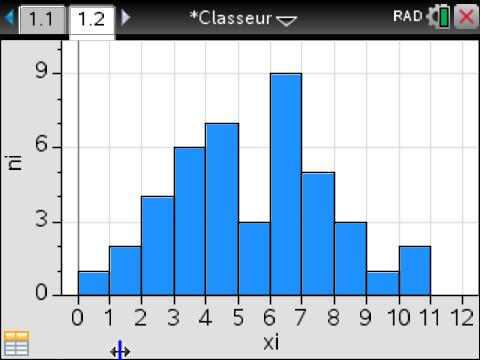
\includegraphics[scale=0.5]{images/histo.jpg}
\caption{Histogramme de la série statistique}
\end{figure}
Je crois que c'est assez explicite. Il faut néanmoins faire attention à une chose : le bâton qui se trouve entre $0$ et $1$ représente bien le nombre de personnes qui ont eu la note $0$ et ainsi de suite
\section{Trois nouveaux outils : variance, écart-type et diagramme en boîte}
\subsection{Variance}
\defi{ : variance d'une série statistique}{On appelle variance de la série statistique et on note $V(x)$ (ou parfois Var($x$)) le nombre $$V(x) = \dfrac{1}{n}\sum_{i=1}^pn_i(x_i-\overline{x})^2 $$}\newline
Autrement dit 
$$V(x) = \dfrac{1}{n}\left(n_1(x_1-\overline{x})^2  + n_2(x_2-\overline{x})^2  + \ldots + n_p(x_p-\overline{x})^2\right)$$
\propriete{}{On a toujours $V(x) \geq 0$}\newline

\begin{preuve}
Somme de termes positifs
\end{preuve}
\prop{}{$$V(x) = \sum_{i=0}^pf_i(x_i-\overline{x})^2 $$}\newline

\begin{preuve}
$$V(x) = \dfrac{1}{n}\sum_{i=0}^p(x_i-\overline{x})^2 n_i = \sum_{i=0}^p(x_i-\overline{x})^2 \dfrac{n_i}{n} = \sum_{i=1}^p(x_i-\overline{x})^2 f_i$$
\end{preuve}

\begin{exemple}
Calculer la variance de l'exemple sur le contrôle\newline

$$V(x) = \begin{array}{l} \dfrac{1}{43}(1\times (0-4,95)^2 + 2 \times (1-4,95)^2 + 4 \times (2-4,95)^2 + 6\times (3-4,95)^2 + 7 \times (4-4,95)^2 + 3 \times (5-4,95)^2 \\+ 9 \times (6-4,95)^2 + 5 \times (7-4,95)^2 + 3\times(8-4,95)^2 + 1 \times (9-4,95)^2 + 2\times (10-4,95)^2) \simeq 5,72\end{array}$$
\end{exemple}

\theo{ : formule de König-Huygens}{On a $$V(x) = \overline{x^2} - \overline{x}^2$$}\newline


\begin{preuve}
L'idée est de développer le $(x_i-\overline{x})^2$ : 
$$V(x) = \dfrac{1}{n}\sum_{i=1}^pn_i(x_i-\overline{x})^2 $$
$$V(x) = \dfrac{1}{n}\sum_{i=1}^p n_i(x_i^2 - 2x_i\overline{x} + \overline{x}^2)$$
$$V(x) = \dfrac{1}{n}(\sum_{i=1}^p n_i x_i^2 - \sum_{i=1}^p 2n_ix_i\overline{x} + \sum_{i=1}^p n_i\overline{x}^2$$
$$V(x) = \dfrac{1}{n}\sum_{i=1}^p n_i x_i^2 - 2\overline{x}\dfrac{1}{n}\sum_{i=1}^p n_ix_i + \overline{x}^2\dfrac{1}{n}\sum_{i=1}^p n_i$$
(on peut sortir les constantes des sommes). \newline Or $\displaystyle \dfrac{1}{n}\sum_{i=1}^p n_i x_i^2 = \overline{x^2}$, $\displaystyle \dfrac{1}{n}\sum_{i=1}^p n_ix_i = \overline{x}$ et $\displaystyle \dfrac{1}{n}\sum_{i=1}^p n_i = 1$ donc 
$$V(x) = \overline{x^2} - 2\overline{x}\times\overline{x} + \overline{x}^2$$
$$V(x) = \overline{x^2} - 2\overline{x}^2 + \overline{x}^2$$
$$V(x) = \overline{x^2} - \overline{x}^2$$
\end{preuve}

La variance sert à mesurer la dispersion des données dans une série statistique : les effectifs dont la valeur est proche de la moyenne n'ont pas beaucoup d'importance dans la variance car $(x_i-\overline{x})^2$ est alors petit. Les effectifs dont la valeur est éloignée de la moyenne, eux, ont une grande importance dans la variance car $(x_i - \overline{x})^2$ est alors grand. Ainsi, plus il y a d'effectifs éloignés de la moyenne, plus la variance est grande avec une évolution linéaire en fonction de l'effectif, quadratique (de manière carrée) en fonction de l'écart à la moyenne
\subsection{Ecart-type}
\defi{ : écart-type}{On appelle écart-type d'une série statistique et on note $\sigma(x)$ le nombre $$\sigma(x) = \sqrt{V(x)}$$}\newline

\prop{ : formules donnant l'écart-type}{$$\sigma(x) = \sqrt{\dfrac{1}{n}\sum_{i=1}^p n_i (x_i - \overline{x})^2}$$ $$\sigma(x) = \sqrt{\sum_{i=1}^p f_i (x_i - \overline{x})^2}$$ $$\sigma(x) = \sqrt{\overline{x^2} - \overline{x}^2}$$}\newline

L'écart type sert lui à mesurer les dispersions dans des données\newline

\begin{exemple}
Dans le cas du contrôle, on a $$\sigma = 2,391$$
\end{exemple}
\subsection{Diagramme en boîte}
Aussi appelé diagramme de boîte à moustache, il permet de rassembler sur un diagramme : $x_{min}, x_{max}, Q_1, Q_2, Q_3$. Voilà à quoi il ressemble et comment le construire : 
\begin{figure}[H]
\centering
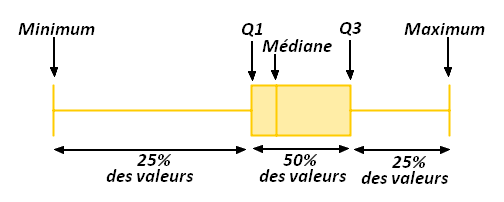
\includegraphics{images/moustache.png}
\caption{Allure d'un diagramme en boîte}
\end{figure}
\methode{pour tracer un diagramme en boîte}{\begin{enumerate} \item Tracer une droite graduée qui couvre au moins l'intervalle $[x_{min},x_{max}]$ \item Placer sur cette droite graduée $x_{min}$, $x_{max}$ ,$Q_1$, $Q_2$ (médiane) et $Q_3$ \item Placer le rectangle et les moustaches(les moustaches sont les segments de $x_{min}$ vers $Q_1$ et de $Q_3$ vers $x_{max}$\end{enumerate}}\newline

\begin{exemple}
Le diagramme en boîte de l'interro est 
\begin{figure}[H]
\centering
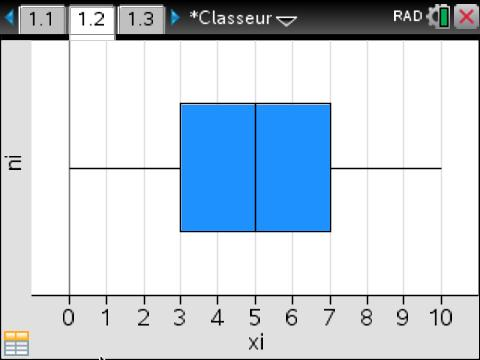
\includegraphics[scale=0.5]{images/moustache_notes.jpg}
\caption{Diagramme en boite de la série statistique de l'interro}
\end{figure}
\end{exemple}
\section{Etudier une série statistique}
Normalement vous serez guidés lorsqu'on vous demandra d'étudier une série statistique. Il faut retenir néanmoins que la moyenne va bien avec l'écart type et la médiane va bien avec l'écart inter-quartiles.\newline

Ne pas oublier que la calculatrice fait très bien les calculs de stats aussi...\newline

\begin{exemple}
On a réuni les tailles des élèves d'un classe : \newline


\begin{tabularx}{\linewidth}{|X|X|X|X|X|X|X|X|}
\hline
Tailles (cm) & 150 & 155 & 160 & 165 & 170 & 175 & 180\\ \hline
Effectif & 3 & 7 & 5 & 5 & 2 & 1&1\\ \hline
\end{tabularx}
\vspace{\baselineskip}
Donner la moyenne, la médiane, les quartiles, l'écart inter-quartiles, l'écart-type, l'histogramme et le diagramme en boite.\newline

Sans justification : 
$$\overline{x} = 163,94$$
$$\sigma = 9,11$$
$$Q_1 = 155$$
$$Q_3 = 170$$
$$M = 165$$
$$Q_3-Q_1 = 15$$
puis 
\begin{figure}[H]
\centering
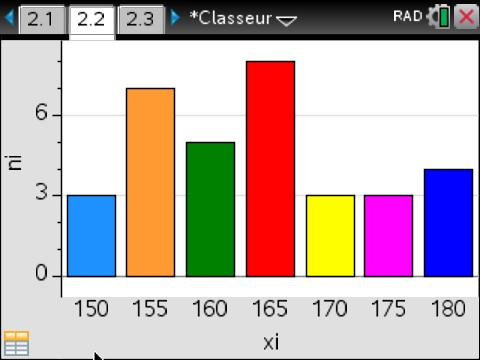
\includegraphics[scale=0.5]{images/recap1.jpg}
\caption{Histogramme}
\end{figure}
\begin{figure}[H]
\centering
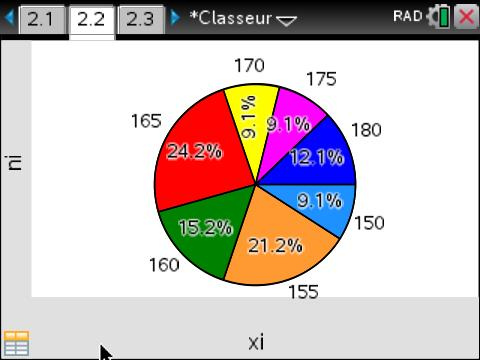
\includegraphics[scale=0.5]{images/recap2.jpg}
\caption{Diagramme circulaire}
\end{figure}
\begin{figure}[H]
\centering
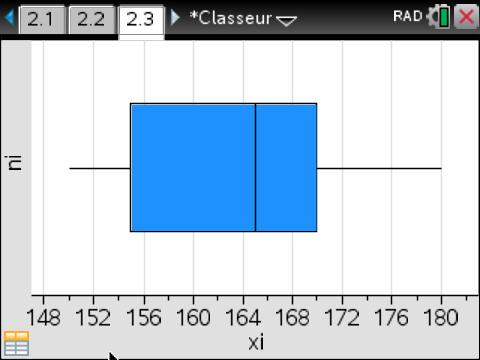
\includegraphics[scale=0.5]{images/recap3.jpg}
\caption{Diagramme en boites}
\end{figure}
\end{exemple}
\begin{remarques}
\begin{itemize}
\item Si la série est donnée sous la forme \newline


\begin{tabularx}{\linewidth}{|X|X|X|X|X|}
\hline
$x_i$ & $[a_1,b_1[$ & $[a_2,b_2[$ & $\ldots$ & $[a_p,b_p[$\\ \hline
$n_i$ & $n_1$ & $n_2$ & $\ldots$ & $n_p$ \\ \hline
\end{tabularx}
alors on applique les résultats précédents (sauf pour l'histogramme) à \newline


\begin{tabularx}{\linewidth}{|X|X|X|X|X|}
\hline
$x_i$ & $x_1=\dfrac{a_1+b_1}{2}$ & $x_2=\dfrac{a_2+b_2}{2}$ & $\ldots$ & $x_p=\dfrac{a_p+b_p}{2}$\\ \hline
$n_i$ & $n_1$ & $n_2$ & $\ldots$ & $n_p$ \\ \hline
\end{tabularx}
\item On demande souvent de calculer l'intervalle $[\overline{x}-\sigma,\overline{x}+\sigma]$ car il contient pas mal d'effectifs... (à méditer)
\end{itemize}
\end{remarques}
\chapter{Probabilités}
\label{chap:proba}
\section{Langage des évènements}
\defi{ : univers}{On réalise une expérience. Une issue est un résultat possible de l'expérience. On appelle univers de cette expérience et on note $\Omega$ l'ensembles des issues possibles}\newline

\begin{exemples}
\begin{itemize}
\item On s'intéresse au lancé d'un dé à six faces. Les résultats possibles sont $1,2,3,4,5,6$ donc $$\Omega = \{1,2,3,4,5,6\}$$
\item On s'intéresse au lancé d'une pièce. les résultats possibles sont "pile" (P) et "face" (F), ainsi $$\Omega = \{P,F\}$$
\item Lors d'un oral d'anglais au bac, le candidat tire au sort un sujet parmi les 4 suivants : Mythes et Héros (H), Environnement (E), Vie en société (S), Mondialisation (M). On a alors $$\Omega = \{H,E,S,M\}$$
\end{itemize}
\end{exemples}
\defi{ : évènement}{Soit $\Omega$ un univers. On appelle évènement une partie de $\Omega$ (c'est-à-dire un ensemble inclus dans $\Omega$)}\newline

On a toujours
$$\varnothing \subset \Omega$$
$$\Omega \subset \Omega$$
donc $\varnothing$ et $\Omega$ sont toujours des évènements\newline

$\varnothing$ est appelé évènement impossible. $\Omega$ est appelé évènement certain.\newline

\begin{exemple}
On reprend l'exemple de l'oral d'anglais \newline

$A$ : "Tirer le sujet sur l'environnement" est un évènement : c'est l'évènement : $A = \{E\} \subset \Omega = \{H,E,S,M\}$\newline

$B$ : "Tirer un sujet qui n'est pas la mondialisation" est un évènement :  $B = \{H,E,S\} \subset \Omega$ \newline

$C$ : "Tirer un sujet de géographie" est un évènement : c'est l'évènement impossible $\varnothing$ \newline

$D$ : "Tirer un sujet qui n'est pas du français" est un évènement : c'est l'évènement certain $\Omega$
\end{exemple}
\propriete{}{Soit $\Omega$ un univers et $A,B$ deux évènements. Alors \begin{itemize}\item $A\cap B$ est un évènement qui correspond à l'évènement  $A$ ET $B$ \item $A\cup B$ est un évènement qui correspond à l'évènement $A$ OU $B$ (OU non exclusif) \item $\overline{A} = \Omega \backslash A$ est un évènement qui correspond à l'évènement $non(A)$\end{itemize}}\newline

\begin{preuve}
Si $A \subset \Omega$ et $B \subset \Omega$ alors $A\cap B\subset \Omega$ et $A\cup B\subset \Omega$\newline

De plus si $A \subset \Omega$ alors $\Omega \backslash A \subset \Omega$\newline

(pour plus de détails : $\leftrightarrows$ raisonnements ensemblistes page \pageref{chap:ensembles})
\end{preuve}
\defi{ : évènements incompatibles}{Soit $A$ et $B$ deux évènements. On dit que $A$ et $B$ sont incompatible si $$A\cap B = \varnothing$$}\newline
\begin{remarques}
\begin{itemize}
\item l'évènement impossible $\varnothing$ est incompatible avec tout évènement
\item $A$ et $\overline{A}$ sont incompatibles car $A\cap(\Omega \backslash A) = \varnothing$
\end{itemize}
\end{remarques}
\begin{exemple}
On lance un dé à six faces 
\begin{enumerate}
\item Donner l'univers $\Omega$
\item On considère les évènements \begin{itemize}\item $A$ : "Obtenir le nombre 4" \item $B$ : "Obtenir un nombre impair" \item $C$ : "Obtenir un nombre différent de 6" \end{itemize} Exprimer $A,B,C$ sous forme d'ensembles
\item Exprimer $A\cup B$, $A \cap B$, $A \cap C$ et $B \cap C$ sous forme d'ensemble et en phrase. En déduire deux évènements incompatibles
\end{enumerate}
\begin{enumerate}
\item $$\Omega = \{1,2,3,4,5,6\}$$
\item $$A = \{4\}$$
$$B = \{1,3,5\}$$
$$C =\{1,2,3,4,5\}$$
\item $A\cup B$ : "Obtenir 4 ou un nombre impair"
$$A \cup B = \{1,3,4,5\}$$
$A \cap B$ : "Obtenir le nombre 4 et un nombre impair
$$A \cap B = \varnothing$$
$A$ et $B$ sont incompatibles\newline

$A \cap C$ : "Obtenir le nombre 4 et un nombre différent de 6"
$$A \cap C = \{4\}$$
$B\cap C$ : "Obtenir un nombre impair différent de 6"
$$B \cap C = \{1,3,5\}$$
\end{enumerate}
\end{exemple}
\section{Probabilités}
On considère 
$$\Omega = \{\omega_1,\omega_2,\ldots,\omega_n\}$$
un univers\newline
Les $\omega_i$ sont appelés évènement élémentaire\newline


\defi{ : probabilité}{On définit une probabilité $P$ sur $\Omega$ en associant à chaque $\omega_i$ un nombre $p_i \in [0,1]$ tel que $\sum_{i=0}^n p_i = 1$. On a alors $$P(\{\omega_i\}) = p_i$$ De plus pour tout $A = \{\omega_{a_1},\omega_{a_2},\ldots,\omega_{a_k}\} = \{\omega_{a_1}\} \cup \{\omega_{a_2}\} \cup \ldots \cup \{\omega_{a_k}\}$ composé d'évènements élémentaires, on a $$P(A) = P(\{\omega_{a_1}\}) + P(\{\omega_{a_2}\}) + \ldots + P(\{\omega_{a_k}\}) = p_{a_1} + p_{a_2} + \ldots + p_{a_k}$$}\newline

\begin{exemple}
On considère un dé truqué dont les probabilités associées sont\newline


\begin{tabularx}{\linewidth}{| X | X | X | X | X | X |}
\hline
1 & 2 & 3 & 4 & 5 & 6 \\ \hline
0,1 & 0,1 & 0,1 & 0,1 & 0,1 & 0,5 \\ \hline
\end{tabularx}


On a bien $0,1 + 0,1 + 0,1 + 0,1 + 0,1 + 0,5 = 1$. L'univers est $\Omega = \{1,2,3,4,5,6\}$. \newline

Calculons les probabilités des évènements suivants : \begin{enumerate}\item $A = \{5\}$ \item $B$ = "Obtenir un nombre pair" \item $C$:"Obtenir un nombre impair" \item $D$:"Obtenir un multiple de $3$" \item $E = B \cap D$\end{enumerate}
\begin{enumerate}
\item $P(A) = P(\{5\}) = 0,1$
\item Les nombres pairs entre $1$ et $6$ sont $2,4,6$ donc $B = \{2,4,6\}$. Ainsi $$P(B) = P(\{2\}) + P(\{4\}) + P(\{6\}) = 0,1+0,1+0,5 = 0,7$$
\item Les nombres impairs entre $1$ et $6$ sont $1,3,5$ donc $C = \{1,3,5\}$. Ainsi $$P(C) = P(\{1\}) + P(\{3\}) + P(\{5\}) = 0,1+0,1+0,1 = 0,3$$
\item Les multiples de $3$ entre $1$ et $6$ sont $3$ et $6$ donc $D = \{3,6\}$. Ainsi $$P(D) = P(\{3\}) + P(\{6\}) = 0,1 + 0,5 = 0,6$$
\item $B \cap D = \{6\}$ donc $P(D) = 0,5$
\end{enumerate}
\end{exemple}
\propriete{}{Soit $\Omega$ un univers et $P$ une probabilité et$A,B$ deux évènements. Alors, on a$$P(\Omega) = 1$$ $$P(\varnothing) = 0$$ $$P(A\cup B) = P(A) + P(B) - P(A\cap B)$$}\newline

\begin{preuve}
\begin{itemize}
\item On a $$\Omega = \{\omega_1,\omega_2,\ldots,\omega_n\}$$ donc $$P(\Omega) = P(\{\omega_1\}) + P(\{\omega_2\}) +\ldots + P(\{\omega_n\})$$
$$P(\Omega) = p_1+p_2+\ldots+p_n = 1$$
\item $\varnothing$ est la réunion d'aucun évènement élémentaire donc $P(\varnothing) = 0$
\item On note 
$$A = \{\omega_{a_1},\omega_{a_2},\ldots,\omega_{a_p},\omega_{c_1},\omega_{c_2},\ldots,\omega_{c_k}\}$$
$$B = \{\omega_{b_1},\omega_{b_2},\ldots,\omega_{b_{p'}},\omega_{c_1},\omega_{c_2},\ldots,\omega_{c_k}\}$$
où $\omega_{c_1},\omega_{c_2},\ldots,\omega_{c_k}$ sont les seuls éléments communs à $A$ et $B$. Ainsi 
$$A \cup B = \{\omega_{a_1},\omega_{a_2},\ldots,\omega_{a_p}, \omega_{b_1},\omega_{b_2},\ldots,\omega_{b_{p'}}, \omega_{c_1},\omega_{c_2},\ldots,\omega_{c_k}\}$$
$$A \cap B = \{\omega_{c_1},\omega_{c_2},\ldots,\omega_{c_k}\}$$
Ainsi 
$$P(A) = p_{a_1} + p_{a_2} + \ldots + p_{a_p} + p_{c_1} + p_{c_2} + \ldots + p_{c_k}$$
$$P(B) = p_{b_1} + p_{b_2} + \ldots + p_{b_{p'}} + p_{a_p} + p_{c_1} + p_{c_2} + \ldots + p_{c_k}$$
$$P(A\cup B) = p_{a_1} + p_{a_2} + \ldots + p_{a_p} + p_{b_1} + p_{b_2} + \ldots + p_{b_{p'}} + p_{c_1} + p_{c_2} + \ldots + p_{c_k}$$
$$P(A\cap B) = p_{c_1} + p_{c_2} + \ldots + p_{c_k}$$
d'où la formule
\end{itemize}
\end{preuve}
\coro{}{Soient $\Omega$ un univers et $P$ une probabilité sur $\Omega$. Si $A$ et $B$ sont incompatibles alors $$P(A\cup B) = P(A) + P(B)$$}\newline

\begin{preuve}
Si $A$ et $B$ sont disjoints alors on a $$A\cap B = \varnothing$$ Ainsi
$$P(A\cup B) = P(A) + P(B) - P(A\cup B) = P(A) + P(B) - P(\varnothing) = P(A) + P(B) - 0 = P(A) + P(B)$$
\end{preuve}
\coro{ : probabilité du complémentaire}{Soient $\Omega$ un univers, $P$ une probabilité sur $\Omega$ et $A$ un évènement. Alors $$P(\overline{A}) = 1 - P(A)$$}\newline

\begin{preuve}
$A$ et $\overline{A}$ étant incompatibles, on a, d'après le corollaire précédent $$P(A\cup \overline{A}) = P(A) + P(\overline{A})$$ or $A\cup \overline{A} = A \cup (\Omega \backslash A) = \Omega$ donc $$1 = P(A) + P(\overline{A})$$ d'ou finalement 
$$P(\overline{A}) = 1 - P(A)$$
\end{preuve}
\begin{exemple}
On considère un dé à 20 faces, truqué, dont les probabilités sont données par \newline


\begin{tabularx}{\linewidth}{| X | X | X | X | X | X | X | X | X | X | X | X | X | X | X | X | X | X | X | X |}
\hline
1 & 2 & 3 & 4 & 5 & 6 & 7 & 8 & 9 & 10 & 11 & 12 & 13 & 14 & 15 & 16 & 17 & 18 & 19 & 20\\ \hline
0,01 & 0,05 & 0 & 0,04 & 0,2 & 0,03 & 0,04 & 0,07 & 0,006 & 0,004 & 0,05 & 0,03 & 0,06 & 0,09 & 0,01 & 0,06 & 0,1 & 0,07 & 0,07 & 0,01\\ \hline
\end{tabularx}
Calculer la probabilité de l'évènement 
$$A : \text{ "Un nombre inférieur ou égal à 17 est tiré" }$$
Pour $\alpha \in [\![1,20]\!]$, on note $A_\alpha$ l'évènement : "le nombre $\alpha$ sort". Ainsi 
$$\Omega = A_1 \cup A_2 \cup \ldots \cup A_{20}$$
On pourrait calculer 
$$P(A_1) + P(A_2) + \ldots + P(A_{17})$$ 
mais ça serait long, du coup on peut calculer 
$$P(\overline{A}) = P(A_{18}) + P(A_{19}) + P(A_{20}) = 0,07 + 0,07 + 0,01 = 0,15$$
Ainsi 
$$P(A) = 1 - P(\overline{A}) = 0,85$$
\end{exemple}
\section{Probabilité uniforme}
Soit $$\Omega = \{\omega_1,\omega_2,\ldots,\omega_n\}$$
un univers $(n\geq 1)$\newline

\defi{ : probabilité uniforme}{On défini la probabilité uniforme par : $$P(\omega_i) = \dfrac{1}{n}$$ pour tout $i \in [\![1,n]\!]$}\newline

\begin{preuve}
On vérifie que c'est bien une probabilité : 
$$n\geq 1$$
donc 
$$0 \leq \dfrac{1}{n} \leq 1$$
Ainsi $$p_i = P(\omega_i) \in [0,1]$$
De plus 
$$\sum_{i=0}^n P(\omega_i) = \sum_{i=0}^n \dfrac{1}{n} = \dfrac{n}{n} =1$$ 
\end{preuve}
Ainsi si $$A = \{\omega_{a_1},\omega_{a_2},\ldots,\omega_{a_p}\}$$
alors $$P(A) = \dfrac{p}{n}$$
$(p \leq n)$\newline

ou autrement dit
$$P(A) = \dfrac{\text{Nombre de cas favorables}}{\text{Nombre de cas total}}$$
Lorsqu'on utilise la probabilité uniforme, on parle de situation équiprobable\newline

\begin{exemple}
On considère un dé équilibré (donc munit de la probabilité uniforme)\newline

Calculer la probabilité des évènements suivants :
\begin{enumerate}
\item $A$ : "Le nombre tiré est 4"
\item $B$ : "Le nombre obtenu est pair"
\item $C$ : "Le nombre obtenu est divisible par 5 ou 2"
\end{enumerate}
\begin{enumerate}
\item $P(A) = \dfrac{1}{6}$
\item $P(B) = \dfrac{3}{6} = \dfrac{1}{2}$
\item $P(C) = \dfrac{3 + 1}{6} = \dfrac{2}{3}$
\end{enumerate}
\end{exemple}
\chapter{Variables aléatoires}
Le cours sur les probabilités ($\leftrightarrows$ page : \pageref{chap:proba}) est nécessaire pour le cours sur les variables aléatoires.
\section{Définition et premières propriétés}
\defi{ : variable aléatoire}{Soit $\Omega = \{\omega_1,\omega_2,\ldots,\omega_n\}$ un univers muni d'une probabilité $P$. On définit une variable aléatoire $X$ sur $\Omega$ en associant à chaque évènement élémentaire $\omega_i$ un nombre réel $x_i$ ($i \in [\![1,n]\!]$). On note alors $X(\Omega) = \{x_1,x_2,\ldots,x_n\}$ l'ensemble des nombres réels ainsi obtenus}\newline

$(X = x_i)$ est un évènement. On peut alors définir $P(X = x_i)$\newline

\defi{ : loi d'une variable aléatoire}{Soit $X$ un variable aléatoire sur $\Omega$. On appelle loi de probabilité de $X$ la donnée de $P(X=x_1), P(X=x_2),\ldots,P(X=x_n)$}\newline

On peut alors donner la loi de $X$ à l'aide d'un tableau\newline


\begin{tabularx}{\linewidth}{| X | X | X | X | X |}
\hline
$x$ & $x_1$ & $x_2$ & $\ldots$ & $x_n$ \\ \hline
$P(X=x)$ & $P(X=x_1)$ & $P(X=x_2)$ & $\ldots$ & $P(X=x_n)$\\ \hline
\end{tabularx}\newline


\begin{exemples}
\begin{enumerate}
\item 
On considère le jeu suivant : on lance un dé équilibré à six faces. Si le résultat est impair, on perd, en euros, le résultat indiqué et si le résultat est pair on le gagne. On note $X$ le gain (c'est-à-dire la variable aléatoire qui compte combien on gagne)
\begin{enumerate}
\item Donner l'univers $\Omega$
\item Donner $X(\Omega)$
\item Donner la loi de $X$
\end{enumerate}
\begin{enumerate}
\item L'univers étant l'ensemble des résultats possibles, on a $$\Omega = \{1,2,3,4,5,6\}$$
\item $X(\Omega)$ représente l'ensemble des valeurs que peut prendre $X$ ainsi $$X(\Omega) = \{-1,+2,-3,+4,-5,+6\} = \{-5,-3,-1,2,4,6\}$$
\item Il faut se demander pour chaque $x\in X(\Omega)$ quelle est la probabilité d'obtenir $x$. Par exemple, quelle est la probabilité de perdre 1 euros. Pour perdre 1 euros, il faut tomber sur $1$. Ainsi $$P(X=-1) = \dfrac{1}{6}$$En fait, on a même, pour tout $x\in X(\Omega)$, $$P(X=x) = \dfrac{1}{6}$$
\begin{tabularx}{\linewidth}{| X | X | X | X | X | X | X |}
\hline
$x$ & $-5$ & $-3$ & $-1$ & $2$ & $4$ & $6$ \\ \hline
$P(X=x)$ & $\dfrac{1}{6}$ & $\dfrac{1}{6}$ & $\dfrac{1}{6}$ & $\dfrac{1}{6}$ & $\dfrac{1}{6}$ & $\dfrac{1}{6}$ \rule[-7pt]{0pt}{20pt} \\ \hline
\end{tabularx}\newline
\end{enumerate}
\item On considère ici, que pour une naissance, la probabilité d'avoir un garçon est de $0,6$ et celle d'avoir une fille est de $0,4$. On considère une famille de $3$ enfants et note $Y$ le nombre de fille 
\begin{enumerate}
\item Quels sont les valeurs que peut prendre $Y$
\item Donner la loi de $Y$
\end{enumerate}
\begin{enumerate}
\item $Y$ peut prendre les valeurs 0,1,2 et 3
\item On réalise un arbre de probabilité\newline
\begin{figure}[H]
\centering
\begin{tikzpicture}
\tikzstyle{lettre}=[fill=white]
\draw (0,3.5) -- (2,5.5) node[style=lettre] {G} node[midway,style=lettre]{$0,6$};
\draw (0,3.5) -- (2,1.5) node [style=lettre] {F} node[midway,style=lettre]{$0,4$};
\draw(2.2,5.5) -- (4,6.5) node[style=lettre] {G} node[midway,style=lettre]{$0,6$};
\draw (2.2,5.5) -- (4,4.5) node[style=lettre] {F} node[midway,style=lettre]{$0,4$};
\draw(2.2,1.5) -- (4,2.5) node[style=lettre] {G} node[midway,style=lettre]{$0,6$};
\draw (2.2,1.5) -- (4,0.5) node[style=lettre] {F} node[midway,style=lettre]{$0,4$};
\draw(4.2,6.5) -- (6,7) node[style=lettre] {G} node[midway,style=lettre]{$0,6$};
\draw(4.2,6.5) -- (6,6) node[style=lettre] {F} node[midway,style=lettre]{$0,4$};
\draw(4.2,4.5) -- (6,5) node[style=lettre] {G} node[midway,style=lettre]{$0,6$};
\draw(4.2,4.5) -- (6,4) node[style=lettre] {F} node[midway,style=lettre]{$0,4$};
\draw(4.2,2.5) -- (6,3) node[style=lettre] {G} node[midway,style=lettre]{$0,6$};
\draw(4.2,2.5) -- (6,2) node[style=lettre] {F} node[midway,style=lettre]{$0,4$};
\draw(4.2,0.5) -- (6,1) node[style=lettre] {G} node[midway,style=lettre]{$0,6$};
\draw(4.2,0.5) -- (6,0) node[style=lettre] {F} node[midway,style=lettre]{$0,4$};
\end{tikzpicture}
\caption{Arbre de probabilité modélisation la situation ci-dessus}
\end{figure}

Le cas $0$ fille se produit dans le cas GGG ainsi $P(Y=0) =  0,6 \times 0,6 \times 0,6 = 0,216$\newline

Le cas $1$ fille se produit dans les cas GGF, GFG, et FGG, ainsi $P(Y=1) = (0,6 \times 0,6 \times 0,4) + (0,6 \times 0,4 \times 0,6) + (0,4 \times 0,6 \times 0,6) = 0,432$\newline

Le cas $2$ filles se produit dans les cas GFF, FGF et FFG ainsi $P(Y=2) = (0,6 \times 0,4 \times 0,4) + (0,4 \times 0,6 \times 0,4) + (0,4 \times 0,4 \times 0,6) = 0,288$\newline

Le cas $3$ filles se produit dans le cas FFF, ainsi $P(Y=3) = 0,4 \times 0,4 \times 0,4 = 0,064$\newline

\begin{tabularx}{\linewidth}{| X | X | X | X | X |}
\hline
$y$ & $0$ & $1$ & $2$ & $3$ \\ \hline
$P(Y=y)$ & $0,216$ & $0,432$ & $0,288$ & $0,064$\\ \hline
\end{tabularx}\newline
Le cas le plus probable est d'avoir une fille
\end{enumerate}
\end{enumerate}
\end{exemples}
\propriete{}{Soit $X$ une variable aléatoire sur $(\Omega,P)$, alors $$P(X=x_1) + P(X=x_2) + \ldots + P(X=x_n) = 1$$}\newline

Autrement dit
$$\sum_{k=1}^n P(X=x_k) = 1$$
ou encore 
$$\sum_{x\in X(\Omega)} P(X=x) = 1$$
\propriete{}{Soient $X$ et $Y$ deux variables aléatoires sur $(\Omega,P)$ et $\lambda \in \R$. Alors \begin{itemize}\item $X+Y$ est une variable aléatoire sur $(\Omega,P)$ \item $\lambda X$ est une variable aléatoire sur $(\Omega,P)$ \end{itemize}}\newline

\propriete{}{Plus généralement si $X$ est une variable aléatoire sur $(\Omega,P)$ et $f$ une fonction telle que $X(\Omega) \subset \mathscr{D}_f$ alors $f(X)$ est une variable aléatoire sur $(\Omega,P)$}\newline 

Par exemple si $X$ est une variable aléatoire, alors $X^2$ aussi
\section{Espérance, variance et écart-type d'une variable aléatoire}
\subsection{Espérance d'une variable aléatoire}
\defi{ : espérance d'une variable aléatoire}{Soit $X$ une variable aléatoire sur $(\Omega,P)$ avec $X(\Omega) = \{x_1,x_2,\ldots,x_n\}$. On appelle espérance de $X$ et on note $E(X)$ le nombre $$E(X) = x_1P(X=x_1) + x_2P(X=x_2)+\ldots x_nP(X=x_n)$$}\newline

Autrement dit
$$E(X) = \sum_{k=1}^n x_kP(X=x_k)$$
ou encore 
$$E(X) = \sum_{x\in X(\Omega)} xP(X=x)$$

\begin{exemples}
On reprend les exemples précédent : 
\begin{enumerate}
\item 
$$E(X) = -5\times P(X=-5) + (-3)\times P(X=-3) + (-1)\times P(X=-1) + 2\times P(X=2) + 4\times P(X=4) + 6\times P(X=6)$$
$$E(X) =  -5\times \dfrac{1}{6}+ (-3)\times \dfrac{1}{6} + (-1)\times \dfrac{1}{6} + 2\times \dfrac{1}{6} + 4\times \dfrac{1}{6} + 6\times \dfrac{1}{6}$$
$$E(X) = \dfrac{1}{2}$$
\item 
$$E(Y) = 0 \times 0,216 + 1\times 0,432 + 2\times 0,288 + 3\times 0,064$$
$$E(Y) = 1,136$$
\end{enumerate}
\end{exemples}
L'espérance peut s'interpréter comme une moyenne, ou dans le cas de gains, ce que l'on peut espérer gagner. Par exemple, en jouant au jeu des des dés, on peut espérer gagner 50 centimes. Ce n'est en fait pas possible de gagner 50 centimes sur 1 tour, mais si on joue un grand nombre $N$ de fois, alors le gain total divisé par $N$ sera proche de 50 centimes : en moyenne, par tour, on aura gagné 50 centimes. \newline

De même pour la situation des enfants : en moyenne un couple qui a 3 enfants aura 1,136 fille (et c'est bien une moyenne, à part si ce sont des gros psychopathes qui découpent des enfants...)\newline

Dans les casino, les jeu ont une espérance négative assez proche de 0 (pour le joueur), de manière à ce qu'en moyenne il perde de l'argent, mais pas trop d'un coup pour qu'il revienne jouer\newline


\begin{exemple}
On considère un jeu : on lance deux dés, si la somme est 2 ou 12, on gagne 30 euros, sinon on perd 2 euros. La probabilité d'obtenir un 12 (ou un 2) est de $\dfrac{1}{6}\times \dfrac{1}{6}= \dfrac{1}{36}$. Ainsi $P(X=30) = \dfrac{1}{36} + \dfrac{1}{36} = \dfrac{2}{36}$ et $P(X = -2) = P(X\neq 30) = 1 - \dfrac{2}{36} = \dfrac{34}{36}$. Ainsi $$E(X) = 30\times \dfrac{2}{36} - 2 \times \dfrac{34}{36} = \dfrac{-8}{36} \simeq -0,22$$
Conclusion : il ne faut pas jouer à ce jeu, même si on a l'impression qu'on peut gagner beaucoup d'un coup
\end{exemple}
\methode{pour déterminer s'il faut jouer à un jeu}{\begin{enumerate}\item Considérer la variable aléatoire $X$ qui compte l'argent gagné (gain) \item Etablir la loi de $X$ \item Calculer $E(X)$ \item \begin{enumerate}\item Si $E(X) >0$ on peut y aller car on va gagner du fric \item Si $E(X) = 0$, c'est un jeu entre potes, on peut y aller aussi \item Si $E(X) < 0$, on y va pas, on va perdre du fric \end{enumerate} \end{enumerate}}\newline

\propriete{}{Soit $X$ une variable aléatoire sur $(\Omega,P)$ et $a,b$ deux réels. Alors $$E(aX+b) = aE(X) +b$$}\newline

\begin{preuve}
On note $X(\Omega) = \{x_1,x_2,\ldots,x_n\}$,\newline $Y = aX+b$,\newline $Y(\Omega) = \{ax_1+b,ax_2+b,\ldots,ax_n+b\} = \{y_1,y_2,\ldots,y_n\}$\newline


Pour tout $k \in [\![1,n]\!]$, on a $X = x_k \Leftrightarrow aX = ax_k \Leftrightarrow aX+b = ax_k +b$ ainsi 
$$P(X = x_k) = P(Y=y_k)$$
Ainsi 
$$E(Y) = \sum_{k=1}^n y_k P(Y=y_k)$$
$$E(Y) = \sum_{k=1}^n (ay_k+b) P(X=x_k)$$
$$E(Y) = \sum_{k=1}^n ax_kP(X=x_k) + \sum_{k=1}^n bP(X=x_k)$$
$$E(Y) = a\sum_{k=1}^n x_k P(X = x_k) + b\sum_{k=1}^n P(X=x_k)$$
or 
$$\sum_{k=1}^n x_k P(X = x_k)  = E(X)$$
et 
$$\sum_{k=1}^n P(X=x_k) = 1$$ donc 
$$E(Y) = aX+b$$

Preuve sans le signe somme $\Sigma$ : 
$$E(Y) = y_1P(Y=y_1) + y_2P(Y=y_2) + \ldots + y_nP(Y=y_n)$$
$$E(Y) = (ax_1+b)P(X=x_1) + (ax_2+b)P(X=x_2) + \ldots + (ax_n+b)P(X=x_n)$$
$$E(Y) = ax_1P(X=x_1) + bP(X=x_1) + ax_2P(X=x_2) + bP(X=x_2) + \ldots + ax_nP(X=x_n) + bP(X=x_n)$$
$$E(Y) = a(x_1P(X=x_1)+ x_2P(X=x_2) + \ldots + x_nP(X=x_n)) + b(P(X=x_1)+ P(X=x_2) + \ldots + P(X=x_n)$$
$$E(Y) = aE(X) + b$$
\end{preuve}
\subsection{Variance et écart-type d'une variable aléatoire}
\defi{ : variance d'une variable aléatoire}{Soit $X$ une variable aléatoire sur $(\Omega,P)$. On note $\mu = E(X)$. On appelle variance de $X$ et on note $V(X)$ le nombre $$V(X) = E((X-\mu)^2)$$}\newline
Autrement dit, 
$$V(X) = E((X-E(X)^2)$$
ou encore
$$\boxed{V(X) = (x_1 - \mu)^2P(X=x_1) + (x_2-\mu)^2P(X=x_2) + \ldots + (x_n - \mu)^2P(X=x_n)}$$
Cette dernière formule nécessite de montrer que $P(X=x_k) = P(Y = y_k)$ où $Y = (X-\mu)^2$, ce qui n'est pas très difficile...\newline


\begin{exemples}
On reprend les exemples du jeu à 2 dés et des enfants
\begin{enumerate}
\item On sait que $E(X) = \dfrac{1}{2}$. Ainsi $$V(X) = \left(-1-\dfrac{1}{2}\right)^2\dfrac{1}{6} + \left(2-\dfrac{1}{2}\right)^2\dfrac{1}{6} + \left(-3-\dfrac{1}{2}\right)^2\dfrac{1}{6} + \left(4-\dfrac{1}{2}\right)^2\dfrac{1}{6} + \left(-5-\dfrac{1}{2}\right)^2\dfrac{1}{6} + \left(6-\dfrac{1}{2}\right)^2\dfrac{1}{6} = \dfrac{179}{12}$$
\item On sait que $E(Y) = 1,136$. Ainsi 
$$V(Y) = (0-1,136)^2\times0,216 + (1-1,136)^2\times0,432+(2-1,136)^2\times0,288 + (3-1,136)^2\times0,064 \simeq 0,724$$
\end{enumerate}
\end{exemples}
\propriete{}{Si $X$ est une variable aléatoire, alors $$V(X) \geq 0$$}\newline


\begin{preuve}
Y a-t-il vraiment besoin d'une preuve ?! (somme de nombres positifs)
\end{preuve}

\defi{ : écart-type d'une variable aléatoire}{Soit $X$ une variable aléatoire sur $(\Omega,P)$. On appelle écart-type de $X$ et on note $\sigma(X)$ le nombre $$\sigma(X) = \sqrt{V(X)}$$}\newline

C'est bien défini car $V(X) \geq 0$

\propriete{}{Soit $X$ une variable aléatoire sur $(\Omega,P)$ et $a\in\R$. Alors $$V(aX) = a^2V(X)$$$$\sigma(aX) = a\sigma(X)$$}\newline

\begin{preuve}
$$V(aX) = E((aX - E(aX))^2) = E((aX-aE(X))^2) = E(a^2(X-E(X))^2) = a^2E((X-E(X)^2)=a^2V(X)$$
$$\sigma(aX) = \sqrt{V(aX)} = \sqrt{a^2V(X)} = a\sqrt{V(X)} = a\sigma(X)$$
\end{preuve}
La variance et l'écart-type sont deux outils pour mesurer l'écartement des valeurs de $X$ par rapport à son espérance (à sa moyenne). Ainsi une variance (ou écart-type) proche de 0 est synonyme de valeurs très proches de l'espérance et une grande variance (ou un grand écart-type) est synonyme d'un écartement des valeurs de $X$
\section{Lois usuelles}
\subsection{Loi uniforme}
\defi{ : loi uniforme}{Soit $X$ une variable aléatoire sur $(\Omega,P)$ avec $X(\Omega) = \{x_1,x_2,\ldots,x_n\}$. On dit que $X$ suit la loi uniforme si, pour tout $k \in [\![1,n]\!]$, $$P(X=x_k) = \dfrac{1}{n}$$}\newline

\begin{exemple}
L'exemple des deux dés qu'on se trimbale depuis le début du chapitre suit la loi uniforme
\end{exemple}

Si $X$ suit la loi uniforme, on note parfois $X \sim \mathscr{U}$\newline

Si $X\sim \mathscr{U}$, alors 
$$E(X) = \dfrac{1}{n}\sum_{k=1}^n x_k$$
(c'est la moyenne des $x_k$)
\subsection{Loi de Bernoulli}
\defi{ : épreuve de Bernoulli}{On appelle épreuve de Bernoulli une expérience aléatoire qui possède deux issues : un succès et un échec}\newline

\begin{exemple}
\begin{enumerate}
\item Le lancer d'une pièce peut être considérer comme une épreuve de Bernoulli si on considère que FACE est un succès et PILE un échec (ou inversement d'ailleurs)
\item On lance un dé à six faces. On dit qu'on a réussi si on tire un 6 et qu'on a échoué si on tire autre chose. C'est une épreuve de Bernoulli
\end{enumerate}
\end{exemple}

\defi{Loi de Bernoulli}{Soit $X$ une variable aléatoire sur $(\Omega,P)$ et $p\in [0,1]$. On dit que $X$ suit la loi de Bernoulli de paramètre $p$ si $$\left\{\begin{array}{l}X\text{ vaut 0 avec une probabilité } (1-p) \\X\text{ vaut 1 avec une probabilité } p \end{array}\right.$$}\newline

Autrement dit 
$$X(\Omega) = \{0,1\}$$et$$P(X=0)=1-p$$ $$P(X=1)=p$$

Si $X$ suit la loi de Bernoulli de paramètre $p$, on note $$X \sim \mathscr{B}(p)$$

\prop{ : espérance d'une variable aléatoire qui suit une loi de Bernoulli}{Soit $X$ une variable aléatoire sur $(\Omega,P)$ telle que $X\sim\mathscr{B}(p)$, alors $$E(X) = p$$}\newline

\begin{preuve}
Si $X \sim \mathscr{B}(p)$, alors 
$$E(X) = 0\times P(X=0) + 1 \times P(X=1) =p$$
\end{preuve}

\prop{ : variance d'une variable aléatoire qui suit une loi de Bernoulli}{Soit $X$ une variable aléatoire sur $(\Omega,P)$ telle que $X\sim\mathscr{B}(p)$, alors $$V(X) = p(1-p)$$}\newline

\begin{preuve}
Si $X\sim \mathscr{B}(p)$, 
$$V(X) = (0-p)^2\times (1-p) + (1-p)^2 \times p = p^2(1-p)+(1-p)^2p=p(1-p)[p+1-p] = p(1-p)$$
\end{preuve}

\prop{ : lien entre épreuve de Bernoulli et loi de Bernoulli}{Soit une épreuve de Bernoulli, dont le succès a une probabilité $p\in [0,1]$ d'arriver (l'échec a donc une probabilité 1-p d'arriver). Alors la variable aléatoire qui vaut 1 dans la cas du succès et 0 dans le cas de l'échec suit la loi de Bernoulli de paramètre $p$}

\begin{exemple}
Donner l'espérance et la variance de la variable aléatoire $X$ qui associe 1 lorsqu'on tire un as dans un jeu de 52 cartes et 0 sinon.\newline

$X$ suit la loi de Bernoulli de paramètre $\dfrac{4}{52} = \dfrac{1}{13}$. Donc $E(X) = \dfrac{1}{13}$ et $V(X) = \dfrac{1}{13}\times \dfrac{12}{13} = \dfrac{12}{169}$
\end{exemple}
\subsection{Loi Binomiale}
En fait, on va consacrer une partie entière à la loi binomiale car y'a pas mal de chose à dire
\section{Loi binomiale}
\subsection{A la découverte du triangle de Pascal}
\defi{ : factorielle}{Soit $n\in \N^*$. On appelle factorielle de $n$ (ou factorielle $n$ ou $n$ factorielle) et on note $n!$ le nombre $$n! = 1 \times 2 \times \ldots \times n$$}\newline

On pose de plus $0! = 1$\newline


\propriete{}{Soit $n\in \N$, on a $$n! \times (n+1) = (n+1)!$$}\newline

\begin{preuve}
$$n!\times (n+1) = (1 \times 2 \times \ldots \times n) \times (n+1) = 1 \times 2 \times \ldots \times n \times (n+1) = (n+1)!$$
\end{preuve}
Ainsi 
$$\dfrac{(n+1)!}{n+1} = n!$$
\defi{ : coefficients binomiaux}{Soientt $k$ et $n$ dans $\N$. On définit le nombre $\binom{n}{k}$ (se lit "$k$ parmi $n$") le nombre $$\left\{\begin{array}{l}\binom{n}{k} = \dfrac{n!}{k!(n-k)!} \text{ si } k \leq n \\ 0 \text{ sinon} \end{array}\right.$$}\newline

Ainsi si $k \leq n$
$$\binom{n}{k} = \dfrac{n!}{k!(n-k)!}$$
\propriete{}{Soit $n\in \N$. On a toujours $$\binom{n}{0} = \binom{n}{n} =1$$}\newline

\begin{preuve}
$$\dfrac{n!}{0!(n-0)!} = \dfrac{n!}{n!} = 1$$
$$\dfrac{n!}{n!(n-n)!} = \dfrac{n!}{n!} = 1$$
\end{preuve}
\propriete{}{Soit $n\in\N$ et soit $k\leq n$. On a $$\binom{n}{k} = \binom{n}{n-k}$$}\newline

\begin{preuve}
$$\binom{n}{k} = \dfrac{n!}{k!(n-k)!}$$
$$\binom{n}{n-k} = \dfrac{n!}{(n-k)! (n-(n-k))!} = \dfrac{n!}{(n-k)!k!} = \dfrac{n!}{k!(n-k)!} = \binom{n}{k}$$
\end{preuve}

\propriete{}{Soit $n\in \N$ et $k\leq n$. Alors $$\binom{n}{k} + \binom{n}{k+1} = \binom{n+1}{k+1}$$}\newline

\begin{preuve}
$$\binom{n}{k} + \binom{n}{k+1} = \dfrac{n!}{k!(n-k)!} + \dfrac{n!}{(k+1)!(n-(k+1))!}$$
$$\binom{n}{k} + \binom{n}{k+1} = \dfrac{n!}{k!(n-k)!} + \dfrac{n!}{(k+1)!(n-k-1)!}$$
On réduit ensuite les fractions au même dénominateur
$$\binom{n}{k} + \binom{n}{k+1} = (k+1)\dfrac{n!}{(k+1)!(n-k)!} + (n-k)\dfrac{n!}{(k+1)!(n-k)!}$$
$$\binom{n}{k} + \binom{n}{k+1} = [(k+1) + (n-k)]\times \dfrac{n!}{(k+1)!(n-k)!}$$
$$\binom{n}{k} + \binom{n}{k+1} = (n+1)\times \dfrac{n!}{(k+1)!(n-k)!}$$
$$\binom{n}{k} + \binom{n}{k+1} = \dfrac{(n+1)!}{(k+1)!(n-k)!}$$
$$\binom{n}{k} + \binom{n}{k+1} = \dfrac{(n+1)!}{(k+1)!(n+1-(k+1))!}$$
$$\binom{n}{k} + \binom{n}{k+1} = \binom{n+1}{k+1}$$
\end{preuve}
Cette formule nous conduit au triangle de Pascal : 
\begin{figure}[H]
\centering
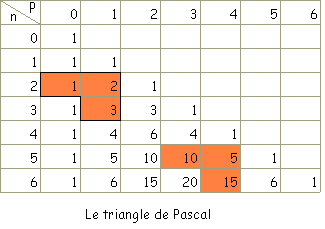
\includegraphics[scale=0.7]{images/pascal1.png}
\caption{Le triangle de Pascal}
\end{figure}
Le coefficient de la ligne $n$ et de la colonne $p$ est $\binom{n}{p}$. D'après la formule, si l'on somme deux nombres en orange d'une ligne, on obtient le nombre en orange de la ligne d'en dessous\newline
(\emph{Source : http://www.bibmath.net/dico/p/images/pascal4.gif})\newline

Une autre représentation du triangle de Pascal est 
\begin{figure}[H]
\centering
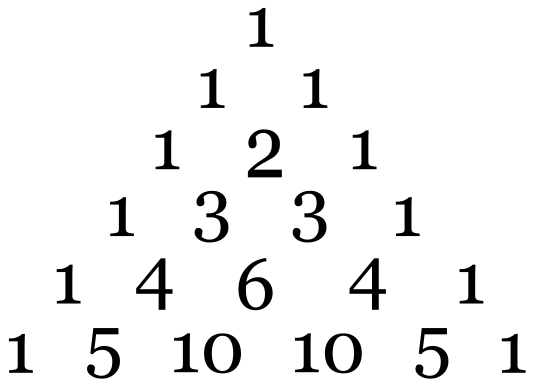
\includegraphics[scale=0.4]{images/pascal2.png}
\caption{Une autre représentation du triangle de Pascal}
\end{figure}
(\emph{Source : wikipédia})\newline
\subsection{Formule du binôme (Hors-programme)}
Bon déjà que la factorielle est à la limite du programme, la formule du binôme de Newton, elle, est complètement hors programme mais intéressante et nous servira pour une preuve plus tard.\newline

Soit $a$ et $b$ deux réels
$$(a+b)^0 = {\color{red} 1}$$
$$(a+b)^1 = {\color{red} 1}\times a+  {\color{red} 1}\times b$$
$$(a+b)^2 = {\color{red} 1}\times a^2+  {\color{red} 2}\times ab + {\color{red} 1}\times b^2$$
$$(a+b)^3 = (a+b)^2(a+b) = (a^2 + 2ab + b^2)(a+b) = a^3 + 2a^2b + b^2a + a^2b + 2ab^2 + b^3$$
$$(a+b)^3 = {\color{red} 1}\times a^3 + {\color{red} 3}\times a^2b + {\color{red} 3}\times ab^2 + {\color{red} 1}\times b^3$$ 
Ne serait-ce pas les coefficients binomiaux ?? \newline
Hé bah non, pour 4 ça marche pas......\newline

Non je déconne, évidemment que c'est les coefficients binomiaux

$$(a+b)^4 = {\color{red} 1}\times a^4 + {\color{red} 4}\times a^3b + {\color{red} 6}\times a^2b^2 + {\color{red} 4}\times ab^3 + {\color{red} 1}\times b^4$$ 
\theo{ : formule du binôme}{Soit $a$ et $b$ deux réels et $n\in \N^*$. Alors $$(a+b)^n = \sum_{k=0}^n \binom{n}{k}a^k b^{n-k}$$}\newline

\begin{preuve}
On fait une preuve par récurrence\newline 

\underline{Initialisation}\newline

$$(a+b)^0 = 1$$
$$\sum_{k=0}^0 \binom{0}{k}a^k b^{n-k} = \binom{0}{0} a^0b^0 = 1$$
Ok\newline

\underline{Héridité}\newline
Soit $n\in \N$ fixé. On suppose 
$$(a+b)^n = \sum_{k=0}^n \binom{n}{k}a^k b^{n-k}$$
On montre alors que c'est vrai pour $n+1$
$$(a+b)^{n+1} = (a+b)^n (a+b)$$
$$(a+b)^{n+1} = \sum_{k=0}^n \binom{n}{k}a^k b^{n-k} (a+b)$$
$$(a+b)^{n+1} = a\sum_{k=0}^n \binom{n}{k}a^k b^{n-k} + b\sum_{k=0}^n \binom{n}{k}a^k b^{n-k}$$
$$(a+b)^{n+1} = \sum_{k=0}^n \binom{n}{k}a^{k+1} b^{n-k} + \sum_{k=0}^n \binom{n}{k}a^k b^{n+1-k}$$
En posant $k+1 = i$ dans la première somme, on obtient 
$$(a+b)^{n+1} = \sum_{i=1}^{n+1} \binom{n}{i-1}a^{i} b^{n-(i-1)} + \sum_{k=0}^n \binom{n}{k}a^k b^{n+1-k}$$
puis en reposant $i = k$ dans la première somme (les indices sont muets...)
$$(a+b)^{n+1} = \sum_{k=1}^{n+1} \binom{n}{k-1}a^{k} b^{n+1-k} + \sum_{k=0}^n \binom{n}{k}a^k b^{n+1-k}$$
$$(a+b)^{n+1} = \binom{n}{n+1-1}a^{n+1}b^{n+1-(n+1)} + \sum_{k=1}^{n} \binom{n}{k-1}a^{k} b^{n+1-k} + \binom{n}{0}a^0b^{n+1-0} \sum_{k=1}^n \binom{n}{k}a^k b^{n+1-k}$$
$$(a+b)^{n+1} = a^{n+1} + b^{n+1} + \sum_{k=1}^{n} \binom{n}{k-1}a^{k} b^{n+1-k} + \sum_{k=1}^n \binom{n}{k}a^k b^{n+1-k}$$
puis en rassemblant les sommes
$$(a+b)^{n+1} = a^{n+1} + b^{n+1} + \sum_{k=1}^{n} \binom{n}{k-1}a^{k} b^{n+1-k} + \binom{n}{k}a^k b^{n+1-k}$$
$$(a+b)^{n+1} = a^{n+1} + b^{n+1} + \sum_{k=1}^{n} a^{k} b^{n+1-k}[\binom{n}{k-1} + \binom{n}{k}]$$
or $\binom{n}{k-1} + \binom{n}{k} = \binom{n+1}{k}$ d'où
$$(a+b)^{n+1} = a^{n+1} + b^{n+1} + \sum_{k=1}^{n} \binom{n+1}{k} a^{k} b^{n+1-k}$$
puis en remettant les $a^{n+1}$ et $b^{n+1}$ dans la somme respectivement comme terme de rang $n+1$ et de rang 0, on obtient finalement
$$(a+b)^{n+1} = \sum_{k=0}^{n+1} \binom{n+1}{k} a^{k} b^{n+1-k}$$
\end{preuve}
\begin{exemple}
Calculer $(a+b)^5$\newline

On regarde les coefficients de la 5-ième ligne du triangle de Pascal : 1 5 10 10 5 1\newline

Ainsi 
$$(a+b)^5 = a^5 + 5a^4b + 10a^3b^2 + 10a^2b^3 + 5ab^4 + b^5$$
\end{exemple}

Les corollaires suivants sont plus pour la culture générale : \newline

\coro{}{Pour tout $n\in\N$ $$\sum_{k=0}^n \binom{n}{k} = 2^n$$}\newline

Autrement dit, la somme des coefficients binomiaux sur une ligne est égale à 2 puissance le numéro de la ligne\newline


\begin{preuve}
$$\sum_{k=0}^n \binom{n}{k} = \sum_{k=0}^n \binom{n}{k}1^k1^{n-k} = (1+1)^n = 2^n$$
\end{preuve}

\coro{}{Pour tout $n\in\N^*$, $$\sum_{k=0}^n (-1)^k \binom{n}{k} = 0$$}\newline


\begin{preuve}
$$\sum_{k=0}^n (-1)^k\binom{n}{k} = \sum_{k=0}^n \binom{n}{k}(-1)^k1^{n-k} = (1-1)^n = 0$$
\end{preuve}
\subsection{Loi binomiale}
\defi{ : loi binomiale}{Soit $X$ une variable aléatoire sur $(\Omega,P)$, $p\in[0,1]$ et $n\in \N^*$. On dit que $X$ suit la loi binomiale de paramètre $n$ et $p$ si $X(\Omega) = \{0,1,2,\ldots,n\}$ et pour tout $k\in [\![0,n]\!]$ $$P(X = k) = \binom{n}{k}p^k(1-p)^{n-k}$$}\newline

Lorsque $X$ suit la loi binomiale de paramètre $n$ et $p$, on note $$X\sim \mathscr{B}(n,p)$$

\begin{remarque}
$$\sum_{k=0}^n P(X = k) = \sum_{k=0}^n \binom{n}{k}p^k(1-p)^{n-k} = (1+(1-p))^n = 1$$
\end{remarque}

\prop{ : espérance de la loi binomiale}{Si $X \sim \mathscr{B}(n,p)$, alors $$E(X) = np$$}\newline

\begin{preuve}
$$E(X) = \sum_{k=0}^n kP(X=k)$$
$$E(X) = \sum_{k=1}^n kP(X=k)$$
$$E(X) = \sum_{k=1}^n k \binom{n}{k} p^k(1-p)^{n-k}$$
$$E(X) = \sum_{k=1}^n k \dfrac{n!}{k!(n-k)!} p^k(1-p)^{n-k}$$
$$E(X) = \sum_{k=1}^n \dfrac{n!}{(k-1)!(n-k)!} p^k(1-p)^{n-k}$$
$$E(X) = np\sum_{k=1}^n \dfrac{(n-1)!}{(k-1)!(n-1-(k-1))!}p^{k-1}(1-p)^{n-1-(k-1)}$$
$$E(X) = np\sum_{k=1}^n \binom{n-1}{k-1}p^{k-1}(1-p)^{n-1-(k-1)}$$
$$E(X) = np\sum_{k=0}^{n-1} \binom{n-1}{k}p^{k}(1-p)^{n-1-(k)}$$
$$E(X) = np(p+(1-p))^{n-1}$$
$$E(X) = np$$
\end{preuve}
Cette preuve n'est pas exigible\newline

\prop{ : variance de la loi binomiale}{Si $X \sim \mathscr{B}(n,p)$, alors $$V(X) = np(1-p)$$}\newline

\subsection{Lien entre loi binomiale et épreuve de Bernoulli}
On réalise $n \in \N^*$ expérience de Bernoulli de paramètre $p\in [0,1]$. On note $X$ le nombre de succès. Alors $X$ suit la loi binomiale de paramètre $n$ et $p$\newline

Comment s'en rendre compte : bah on fait un arbre \newline
\begin{figure}[H]
\centering
\begin{tikzpicture}
\tikzstyle{lettre}=[fill=white]
\draw (0,3.5) -- (2,5.5) node[style=lettre] {S} node[midway,style=lettre]{$p$};
\draw (0,3.5) -- (2,1.5) node [style=lettre] {E} node[midway,style=lettre]{$1-p$};
\draw(2.2,5.5) -- (4,6.5) node[style=lettre] {S} node[midway,style=lettre]{$p$};
\draw (2.2,5.5) -- (4,4.5) node[style=lettre] {E} node[midway,style=lettre]{$1-p$};
\draw(2.2,1.5) -- (4,2.5) node[style=lettre] {S} node[midway,style=lettre]{$p$};
\draw (2.2,1.5) -- (4,0.5) node[style=lettre] {E} node[midway,style=lettre]{$1-p$};
\draw(4.2,6.5) -- (6,7) node[style=lettre] {S} node[midway,style=lettre]{$p$};
\draw(4.2,6.5) -- (6,6) node[style=lettre] {E} node[midway,style=lettre]{$1-p$};
\draw(4.2,4.5) -- (6,5) node[style=lettre] {S} node[midway,style=lettre]{$p$};
\draw(4.2,4.5) -- (6,4) node[style=lettre] {E} node[midway,style=lettre]{$1-p$};
\draw(4.2,2.5) -- (6,3) node[style=lettre] {S} node[midway,style=lettre]{$p$};
\draw(4.2,2.5) -- (6,2) node[style=lettre] {E} node[midway,style=lettre]{$1-p$};
\draw(4.2,0.5) -- (6,1) node[style=lettre] {S} node[midway,style=lettre]{$p$};
\draw(4.2,0.5) -- (6,0) node[style=lettre] {E} node[midway,style=lettre]{$1-p$};
\end{tikzpicture}
\caption{Arbre de probabilité représentant la répétition d'une épreuve de Bernoulli}
\end{figure}
(S : Succès; E: Echec)\newline

Sur un chemin où il y $k$ succès, il y a $k$ branches à $p$ et $n-k$ branches à $n-p$ donc la probabilité d'avoir CE chemin est $p^k(1-p)^{n-k}$. Or il y a $\binom{n}{k}$ chemin avec $k$ succès dont $$P(X=k) = \binom{n}{k} p^k (1-p)^{n-k}$$

Ce résultat permet de comprendre l'espérance et la variance de la loi binomiale en admettant que $E(X+Y) = E(X)+E(Y)$. En effet si l'on note $X_1,X_2,\ldots,X_n$ les variables aléatoires associées à chacune des expériences de Bernoulli. Alors la variable aléatoire $X$ qui compte le nombre de succès lors de la répétition des $n$ épreuves s'écrit comme 
$$X = X_1 + X_2 + \ldots + X_n$$
donc 
$$E(X) = E(X_1 + X_2 + \ldots + X_n)$$
$$E(X) = E(X_1) + E(X_2) + \ldots + E(X_n)$$
$$E(X) = p + p +\ldots + p$$
$$E(X) = np$$
et
$$V(X) = V(X_1 + X_2 + \ldots + X_n)$$
$$V(X) = V(X_1) + V(X_2) + \ldots + V(X_n)$$
$$V(X) = p(1-p) + p(1-p) +\ldots + p(1-p)$$
$$V(X) = np(1-p)$$
\begin{exemple}
On tire une carte dans un jeu de 52 cartes, puis on la remet dans le paquet, et on recommence cette opération $25$ fois. Calculer la probabilité de tirer exactement $3$ fois l'as de coeur\newline

On interprète l'évènement "on tire l'as de coeur" comme un succès de probabilité $\dfrac{1}{52}$. Ainsi la variable aléatoire $X$ qui compte le nombre de fois que l'on tire l'as de coeur suit la loi binomiale de paramètre 25 et $\dfrac{1}{52}$. On déduit 
$$P(X=3) = \binom{25}{3}\left(\dfrac{1}{52}\right)^3\left(\dfrac{51}{52}\right)^{22} = $$
\end{exemple}
\subsection{Représentation de la loi binomiale}
Regardons tout d'abord l'effet du changement de $n$ à $p$ constant. On a pris $p = 0.5$ et $n \in \{10,15,20,40\}$
\begin{figure}[H]
\centering
\includegraphics[scale=0.35]{images/loi_binomiale_1.png}
\caption{Représentation de la loi binomiale pour $p = 0.5$ et $n \in \{10,15,20,40\}$}
\end{figure}
Les traits continus sont les représentations graphiques des fonctions $x\mapsto \binom{n}{x} 0.5^x 0.5^{n-x}$ (après généralisation des puissances non entières et des factorielles non entières que l'on ne fait pas ici) et les points correspondent au $(k,\binom{n}{k} 0.5^k 0.5^{n-k})$ ($k\in [\![0,n]\!]$)\newline

Regardons maintenant l'effet du changement de $p$ à $n$ constant. On a pris $n = 20$ et $p \in \{0.1,0.4,0.7,0.8\}$
\begin{figure}[H]
\centering
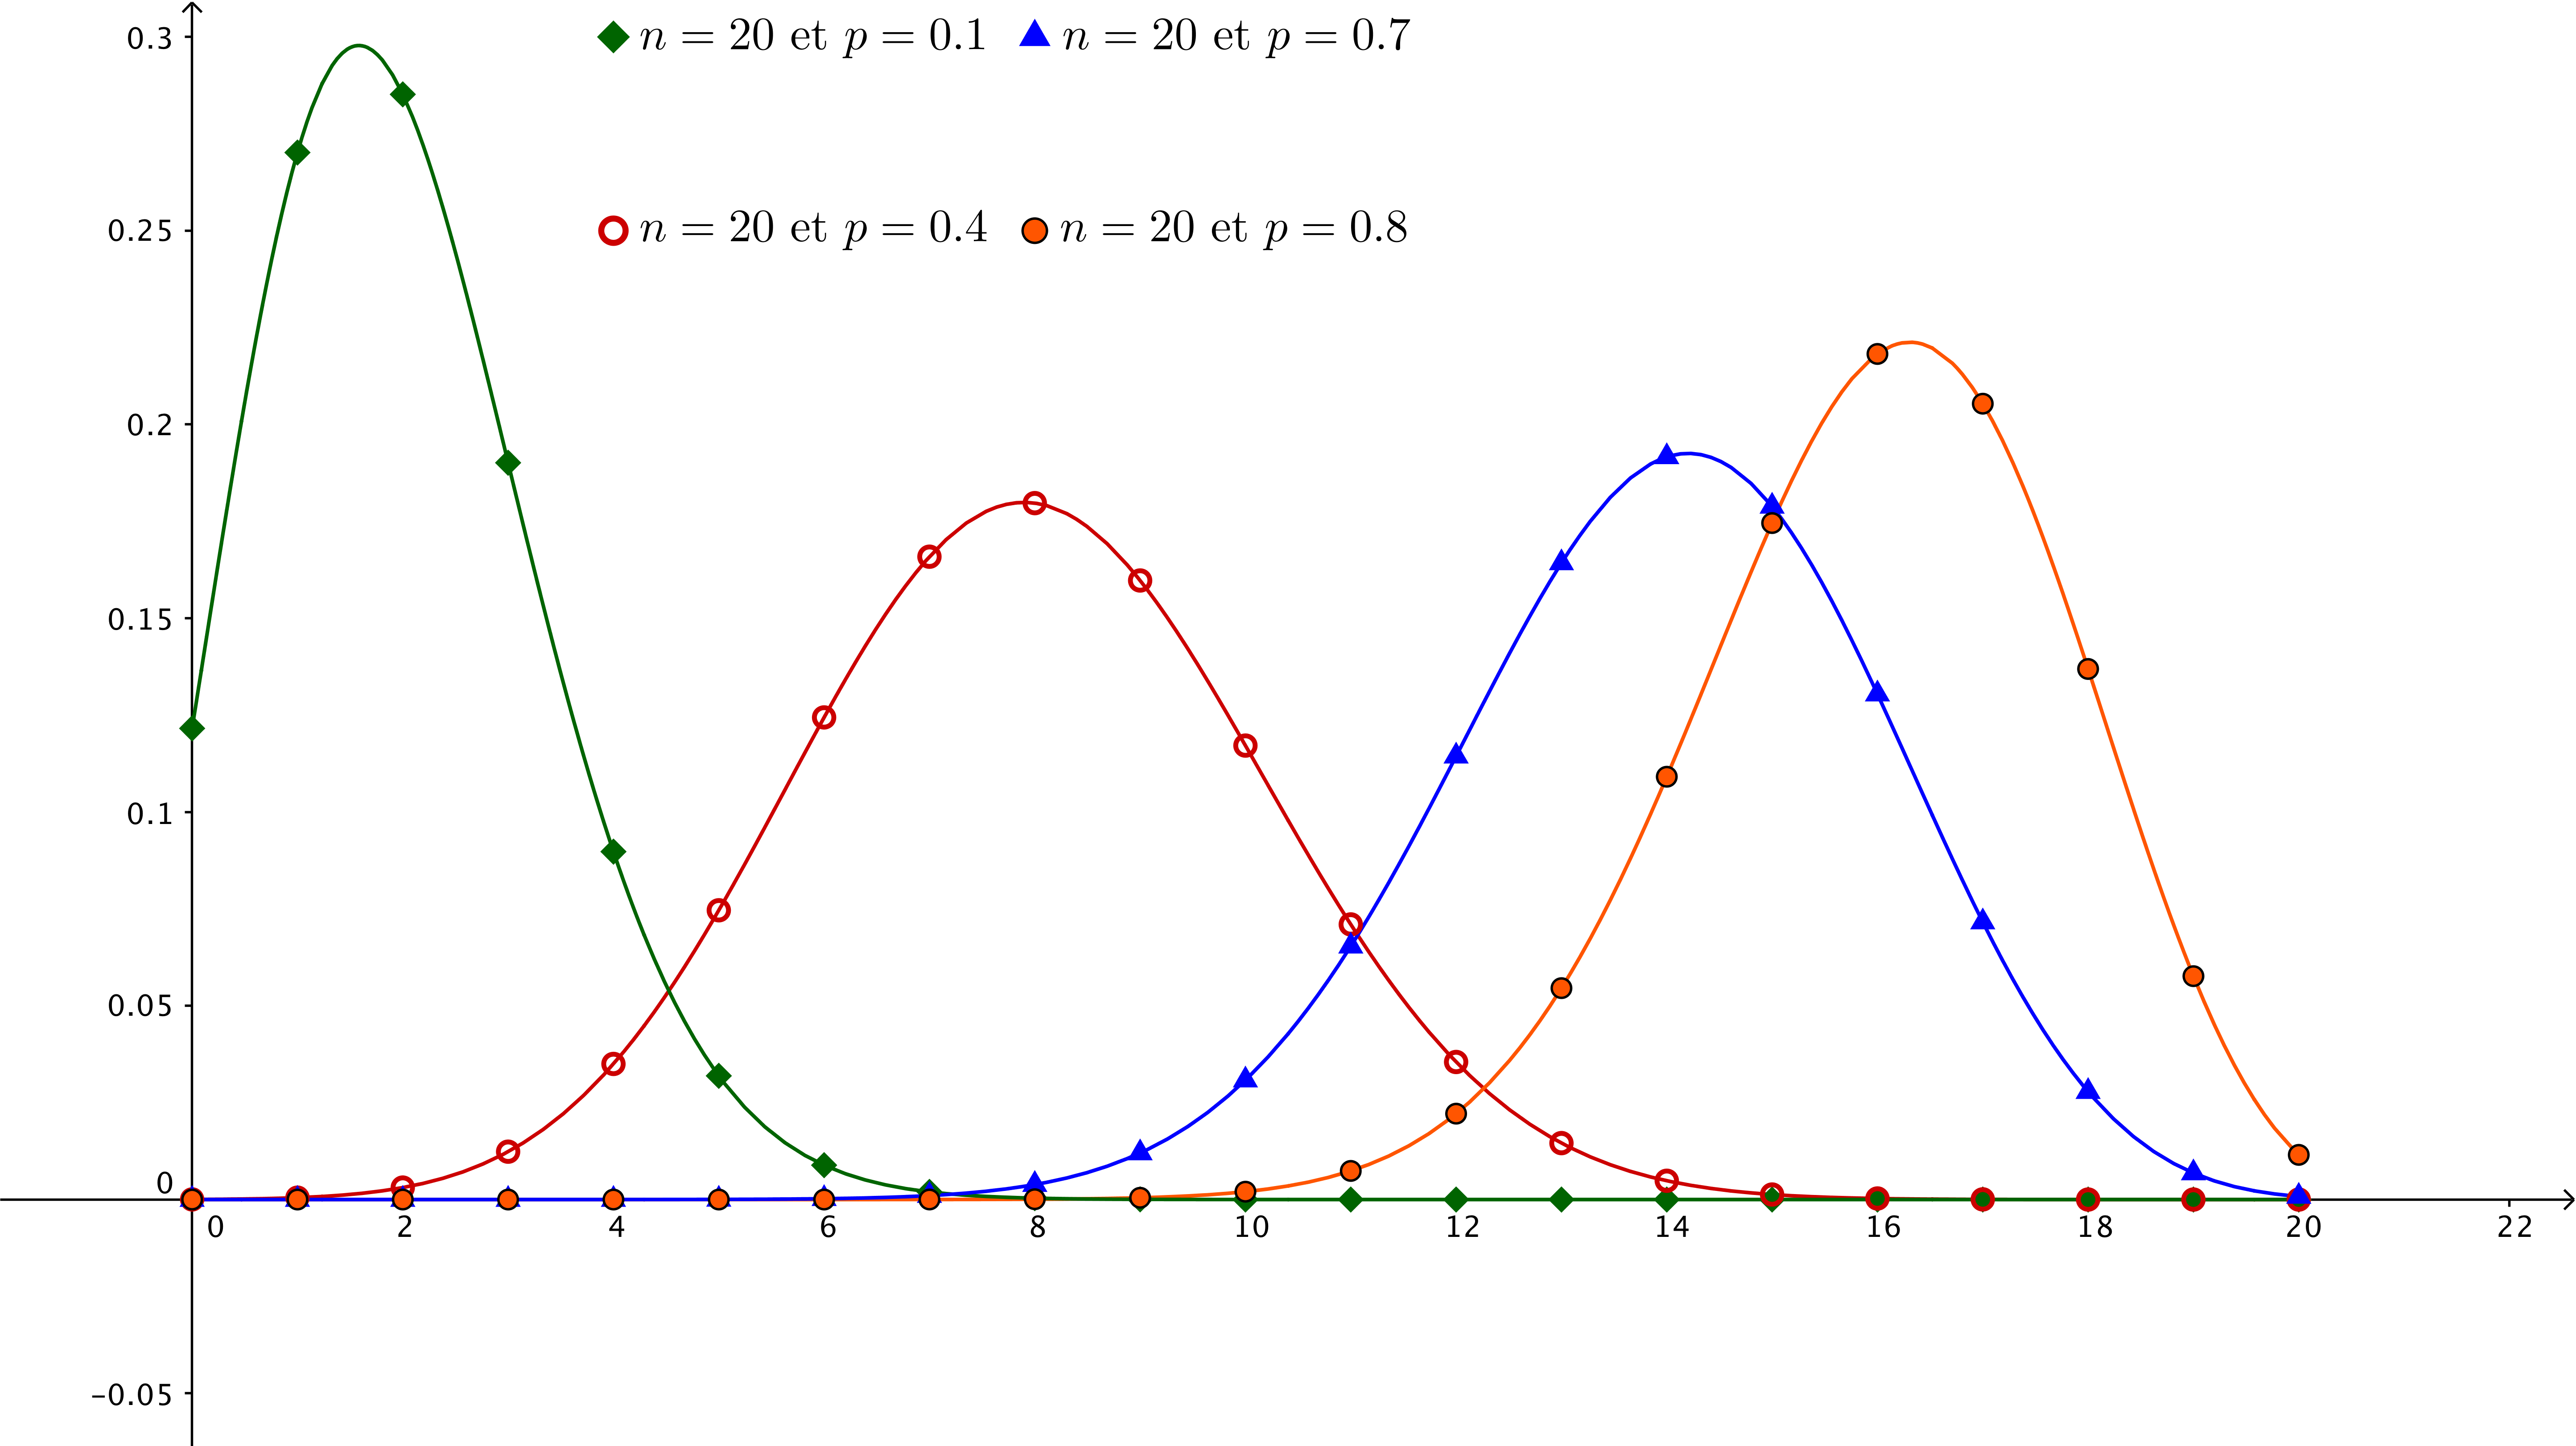
\includegraphics[scale=0.7]{images/loi_binomiale_2.png}
\caption{Représentation de la loi binomiale pour $n = 20$ et $p \in \{0.1,0.4,0.7,0.8\}$}
\end{figure}
Les traits continus sont les représentations graphiques des fonctions $x\mapsto \binom{20}{x} p^x (1-p)^{20-x}$ (après généralisation des puissances non entières et des factorielles non entières que l'on ne fait pas ici) et les points correspondent au $(k,\binom{20}{k} p^k (1-p)^{n-k})$($k\in [\![0,20]\!]$)\newline


Il est important de faire le lien entre probabilités et statistiques sans pour autant mélanger les notions : la notion de fréquence est analogue à la notion de probabilité, la notion de moyenne est analogue à la notion d'espérance, les notions de variances et écart-type en statistiques sont analogues aux notions de variance et écart-type en probabilités.
\chapter{Echantillonage}
\section{Contextualisation}
On considère une population $P$, composées d'individus et on s'intéresse à l'apparition d'un caractère $C$ dans cette population ($\leftrightarrows$ cours sur les statistiques pour le vocabulaire : p. \pageref{chap:stats}). On sait que le caractère $C$ apparait avec une proportion $p$ dans cette population.\newline

On tire au hasard un échantillon de $n$ dans la population $P$. On note alors $f$ la fréquence d'apparition de $C$ dans l'échantillon. Comment savoir si cet échantillon est représentatif de la population ? \newline 

\begin{exemple}
En France, au 4ème trimestre de 2016, il y avait 10\% de chômeurs (source : Insee). On tire au hasard 10000 français et on compte le nombre de chômeurs. Il y a en a 987. Cet échantillon est-il représentatif ?
\end{exemple}
\section{Rappels de seconde}
\theo{}{Soit $C$ un caractère présent dans une proportion $p$ dans une population $P$. On considère un échantillon de taille $n$ de cette population et on note $f$ la fréquence de $C$ dans cet échantillon. On suppose $0,2 \leq p \leq 0,8$ et $n \geq 25$. Alors la probabilité que $f$ soit dans l'intervalle $$\left[p - \dfrac{1}{\sqrt{n}},p + \dfrac{1}{\sqrt{n}}\right]$$ est supérieure ou égale à $0,95$}\newline

Ce qui peut aussi s'écrire 
$$P\left(p - \dfrac{1}{\sqrt{n}} \leq f \leq p + \dfrac{1}{\sqrt{n}}\right) \geq 0,95$$
Vocabulaire : \newline

Si on a tiré un échantillon de taille $n \geq 25$, pour étudier un caractère $C$ de proportion $p$, et que la fréquence de $C$ dans l'échantillon se trouver dans l'intervalle $\left[p - \dfrac{1}{\sqrt{n}},p + \dfrac{1}{\sqrt{n}}\right]$, on dit que \textbf{l'échantillon est représentatif de la population au seuil de confiance de 95\%}\newline

\begin{exemples}
\begin{enumerate}
\item En 2015, en France, 72\% des hommes qui passaient le bac l'ont obtenu (source : Insee). On considère un échantillon de 3000 élèves (de sexe masculin) qui viennent de passer le bac. Parmi eux, 2184 élèves l'ont obtenu
\begin{enumerate}
\item Quel caractère étudie-t-on ?
\item Déterminer l'intervalle de fluctuation au seuil de 95 \% pour ce caractère et cet échantillon
\item Cet échantillon est-il représentatif de la population ? 
\end{enumerate}
\begin{enumerate}
\item On étudie le caractère "avoir obtenu la baccalauréat en 2015"
\item On a bien $3000 \geq 25$ et $0,2 \leq 0,72 \leq 0,8$. Ainsi l'intervalle de fluctuation au seuil de 95\% est 
$$\left[0,72 - \dfrac{1}{\sqrt{3000}};0,72 + \dfrac{1}{\sqrt{3000}}\right]$$
$$\left[0,7;0,73\right]$$
\item Calculons la fréquence $f$ d'apparition du caractère dans cet échantillon : 
$$f = \dfrac{2184}{3000} = 0,728$$
$0,728 \in [0,7;0,73]$ donc cet échantillon est représentatif au seuil de confiance de 95\%
\end{enumerate}
\item En 2016, 48,9\% des femmes ont fait une déclaration à la police après un vol (source : Insee). On considère un échantillon de 500 femmes qui ont été victimes de vols. Parmi elles, 275 l'ont déclaré à la police. Cet échantillon est-il représentatif ?\newline

On étudie le caractère : "avoir déclaré le vol"\newline

On a $500 \geq 25$ et $0,2 \leq 0,489 \leq 0,8$ donc un intervalle de fluctuation au seuil de 95 \% est  
$$\left[0,489 - \dfrac{1}{\sqrt{500}};0,489 + \dfrac{1}{\sqrt{500}}\right]$$
$$\left[0,444;0,533\right]$$
Calculons la fréquence $f$ d'apparition du caractère $C$ dans cet échantillon :
$$f = \dfrac{275}{500} = 0,55$$
$0,55 \notin [0,444;0,533]$ donc cet échantillon n'est pas représentatif au seuil de confiance de 95\%.
\end{enumerate}
\end{exemples}
\methode{pour montrer qu'un échantillon est ou n'est pas représentatif}{\begin{enumerate} \item Rappeler le caractère étudié \item Vérifier que $n\geq 25$ et $0,2 \leq p \leq 0,8$ \item Etablir l'intervalle de fluctuation $$\left[p - \dfrac{1}{\sqrt{n}},p + \dfrac{1}{\sqrt{n}}\right]$$ \item Calculer la fréquence $f$ d'apparition du caractère dans l'échantillon \item Si $f \in [p - \dfrac{1}{\sqrt{n}},p + \dfrac{1}{\sqrt{n}}]$ alors l'échantillon est représentatif au seuil de confiance de 95\%. Sinon il ne l'est pas\end{enumerate}}\newline

\begin{remarques}
\begin{itemize}
\item Plus $n$ est grand, moins l'intervalle est large
\item Si $n \geq 25$ alors $\dfrac{1}{\sqrt{n}} \leq 0,2$. Ainsi, on est sur que 
$$p - \dfrac{1}{\sqrt{n}} \geq 0$$
$$p + \dfrac{1}{\sqrt{n}} \leq 1$$
\end{itemize}
\end{remarques}
\section{Lien avec la loi binomiale}
Soit $C$ un caractère de proportion $p$. On note $S$ le succès "l'individu possède la caractère S". Alors, lorsqu'on tire un individu au hasard, on réalise une expérience de Bernoulli de paramètre $p$. Ainsi en notant $X$ le nombre d'individus possédant le caractère $C$ dans un échantillon de taille $n$, on remarque que $X$ suit la loi binomial de paramètre $n$ et $p$. On s'intéresse alors à la variable aléatoire $F= \dfrac{X}{n}$ qui représente la fréquence aléatoire.\newline

D'après le résultat précédent 
$$P\left(p-\dfrac{1}{\sqrt{n}} \leq F \leq p+\dfrac{1}{\sqrt{n}}\right) \geq 0,95$$
\defi{ : intervalle de fluctuation}{Soit $X$ une variable aléatoire qui suit une loi binomiale $\mathscr{B}(n,p)$ et $F = \dfrac{X}{n}$. Un intervalle de fluctuation de $F$ au seuil de 95 \% est un intervalle \begin{itemize} \item de la forme $[\dfrac{a}{n},\dfrac{b}{n}]$ avec $a$ et $b$ deux entiers entre $0$ et $n$ \item tel que $P\left(\dfrac{a}{n} \leq F \leq \dfrac{b}{n}\right) \geq 0,95$ ce qui équivaut à $P\left(a \leq X \leq b\right) \geq 0,95$\end{itemize}} \newline

\prop{}{Soit $a$ le plus grand entier tel que $P(X \leq a) < 2.5$\%. Soit $b$ le plus petit entier tel que $P(X \leq b) \geq 97.5$\%. Alors $[\dfrac{a}{n},\dfrac{b}{n}]$ est l'intervalle de fluctuation au seuil de 95\%}\newline

\methode{pour établir l'intervalle de fluctuation}{On calcule grâce à un tableau les valeurs de $P(X \leq k)$ ($k\in\N$). On recherche alors les $a$ et $b$ grâce au résultat précédent}\newline

\underline{Prise de décision}\newline
On fait l'hypothèse que le caractère $C$ apparait avec une proportion $p$. On considère un échantillon de taille $n$ où $C$ a une fréquence $f$. Soit $[\dfrac{a}{n},\dfrac{b}{n}]$ l'intervalle de fluctuation au seuil de 95\%.\newline

Si $f\notin[\dfrac{a}{n},\dfrac{b}{n}]$, on rejette l'hypothèse (avec un risque de 5\%)\newline
Si $f\in[\dfrac{a}{n},\dfrac{b}{n}]$, on ne rejette pas l'hypothèse \newline

\begin{exemple}
On admet que la proportion de garçon qui naisse par rapport au total de naissance est de $0,516$. On observe sur un échantillon de taille 50, une fréquence de garçon 0,4\newline

Avec un tableur, on obtient $a=19$ et $b=33$, on en déduit alors l'intervalle de fluctuation à 95\% est $$\left[\dfrac{19}{50},\dfrac{33}{50}\right] = [0,36;0,66]$$
$f\in[0,36;0,66]$ alors on ne rejette pas l'hypothèse
\end{exemple}
\part{Algorithmique et raisonnements ensemblistes}
\chapter{Algorithmique}
\label{chap:algorithmique}
\begin{prog}
\emph{"L'algorithmique a une place naturelle dans tous les champs des mathématiques et les problèmes posés doivent être en relation avec les autres parties du programme (analyse, géométrie, statistiques et probabilités, logique), mais aussi avec les autres disciplines ou le traitement de problèmes concrets.
À l'occasion de l'écriture d'algorithmes et programmes, il convient de donner aux élèves de bonnes habitudes de rigueur et de les entraîner aux pratiques systématiques de vérification et de contrôle."}\newline

\emph{"De même, les activités de type algorithmique sont signalées par le symbole $\lozenge$"}\end{prog}

\begin{remarque}
Il n'y aucune notation officielle concernant la mise en page des algorithmes. Néanmoins on retrouve souvent la présentation
\begin{figure}[H]
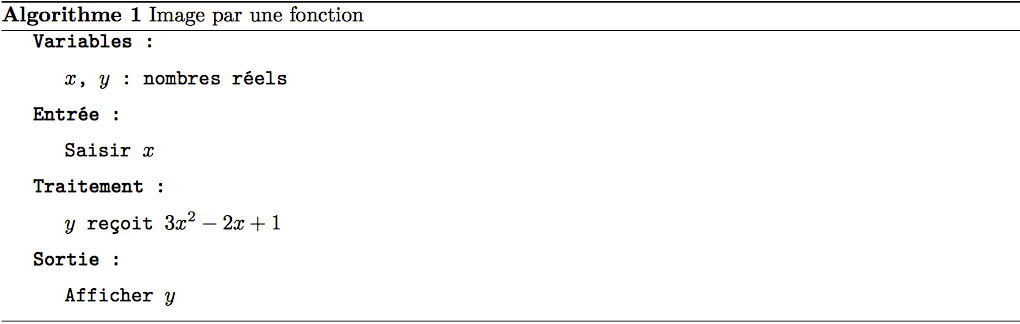
\includegraphics[scale=0.4]{images/autreforme.png}
\caption{Une représentation algorithmique}
\end{figure}
(variables, entrée, traitement, sortie) et il faut la connaitre. Néanmoins, j'ai ici pris le partit d'utiliser algobox, un logiciel d'initiation à la programmation au lycée. (voir algobox sur internet)
\end{remarque}
\section{Cours}
\subsection{Instructions élémentaires}
\textbf{Variables}\newline
Sans revenir fondamentalement sur la notion de variable, une variable, c'est quelque chose qui varie (merci captain obvious) et qui est voué à varier pendant l'exécution de l'algorithme. Chaque variable possède un nom et dans le cas d'algorithme elle possède souvent un type : dans algobox il y a trois types : nombre, liste et chaine. Les nombres on sait ce que sait mais en fait pour algobox, les nombres décimaux. Les listes bah c'est des listes. Les chaine se sont des chaines de caractères (par exemple "salut les amis" est une chaine de caractère). Dans d'autres langages de programmation, on trouve d'autre types comme int (entier), float (nombre décimal), string (chaine caractère), array (tableau, liste), none (aucun type), voire d'autres. La notion de type n'est pas forcément importante mais permet d'appréhender les concepts de programmation. \newline

On pointe l'attention qu'il n'y a pas de type réel ou rationnel : il ne peut pas garder en mémoire des nombres avec une infinité de chiffres après la virgule : il y a une précision.\newline


\textbf{Calculs}\newline
On peut faire des calculs dans un algorithme (merci captain obvious $\times 2$). Dans tous les langages de programmation on retrouve 4 opérations de base : $+$ (somme), $-$ (soustraction), $*$(multiplication), $/$ (division par un nombre non nul) et $\%$ ($a\%b$ renvoie le reste la division euclidienne de $a$ par $b$). Après on trouve différentes notation pour autres opérations selon les langages.


\textbf{Affectation}\newline
On a des variables et logiquement, on peut leur donner une valeur : on parle d'\textbf{affectation}.\newline

\begin{algobox}
\DebutAlgo
\Ligne variable PREND\_LA\_VALEUR valeur
\FinAlgo
\end{algobox}

\textbf{Commentaire}\newline
Il est possible de commenter son code. C'est parfois (mais souvent très peu utilisé dans les algorithmes). Dans quasiment tous les langages de programmation on utilise le // (mais pas tous, par exemple dans celui qui a été utilisé pour écrire ce cours, on utilise le \%)\newline
Ainsi on peut écrire 
\begin{algobox}
\DebutAlgo
\Ligne Traitement
\Ligne // ceci est un commentaire
\Ligne Traitement
\FinAlgo
\end{algobox}
Tout l'intérêt d'un commentaire est de ne pas être exécuté par la machine : le code qui se trouve après // ne sera pas interprété. Par exemple si l'on écrit
\begin{algobox}
\Variables
\Ligne x EST\_DU\_TYPE NOMBRE
\Ligne y EST\_DU\_TYPE NOMBRE
\DebutAlgo
\Ligne SAISIR x
\Ligne y PREND\_LA\_VALEUR 3*x+2
\Ligne // y PREND\_LA\_VALEUR 8
\Ligne AFFICHER y
\FinAlgo
\end{algobox}
\begin{verbatim}
> // Applications de l'algorithme
>
> x = 2
> y = 8
>
> x = 1
> y = 5
\end{verbatim}
\subsection{Instruction conditionnelle}
Regardons d'abord les instructions conditionnelles : Si... Alors... Sinon... (If... Then... Else). Elle s'écrit 
\begin{algobox}
\Si{(condition)}
\DebutSi
\Ligne Traitement 1
\FinSi
\Sinon
\DebutSinon
\Ligne Traitement 2
\FinSinon
\end{algobox} 
Lorsque l'algorithme arrive au SI, il n'exécute le traitement 1 que si la condition est respectée; dans ce cas il n'exécute pas le traitement 2. Si la condition n'est pas respectée, alors il n'exécute pas le traitement 1 et exécute le traitement 2\newline

\begin{exemple}
Dans une famille nombreuse (de 47 enfants), le père en a marre de devoir féliciter ou réprimander ses enfants lorsqu'ils ont une bonne ou mauvaise note. Il écrit alors un programme tel que : l'enfant rentre sa note $N$ dans l'ordinateur : si la note est supérieure (ou égale) à 10, le programme félicite l'enfant, sinon il le réprimande. \newline

La condition est ici $N \geq 10$ (qui s'écrit dans algobox N >= 10). Le traitement 1 correspondra à féliciter l'enfant et le traitement 2 à le réprimander.
\begin{algobox}
\Variables
\Ligne N EST\_DU\_TYPE NOMBRE
\DebutAlgo
\Ligne SAISIR N
\Si{(N >= 10)}
\DebutSi
\Ligne AFFICHER "Félicitations"
\FinSi
\Sinon
\DebutSinon
\Ligne AFFICHER "C'est pas bien"
\FinSinon
\FinAlgo
\end{algobox}
\begin{verbatim}
> // Applications de l'algorithme
>
> N = 12
> "Félicitations"
>
> N = 3
> "C'est pas bien"
\end{verbatim}
\end{exemple}
On peut affiner ces structures avec Si (condition 1) Alors Traitement 1 Sinon Si (condition 2) Alors Traitement 2 Sinon Traitement 3 (If ... Then ... Else if ... Then ... Else ...). Ces structures ne sont pas vraiment au programme mais on peut les créer en emboitant des structures Si ... Alors ... Sinon ... : 
\begin{algobox}
\DebutAlgo
\Si{(condition 1)}
\DebutSi
\Ligne Traitement 1
\FinSi
\Sinon
\DebutSinon
\Si{(condition 2)}
\DebutSi
\Ligne Traitement 2
\FinSi
\Sinon
\DebutSinon
\Ligne Traitement 3
\FinSinon
\FinSinon
\FinAlgo

\end{algobox}
\begin{exemple}
On reprend notre père de famille nombreuse, qui veut que son programme affiche \begin{itemize} \item Très bien si $N \in [15,20]$ \item Bien si $N \in [10,15[$ \item Mauvais si $N \in [5,10[$ \item Très mauvais si $N \in [0,5[$\end{itemize} Pour cela, il nous faut trois structures Si... Alors ... Sinon emboités
\begin{algobox}
\Variables
\Ligne N EST\_DU\_TYPE NOMBRE
\DebutAlgo
\Ligne SAISIR N
\Si{(N < 5)}
\DebutSi
\Ligne AFFICHER "Très mauvais"
\FinSi
\Sinon
\DebutSinon
\Si{(N < 10)}
\DebutSi
\Ligne AFFICHER "Mauvais"
\FinSi
\Sinon
\DebutSinon
\Si{(N < 15)}
\DebutSi
\Ligne AFFICHER "Bien"
\FinSi
\Sinon
\DebutSinon
\Ligne AFFICHER "Très bien"
\FinSinon
\FinSinon
\FinSinon
\FinAlgo
\end{algobox}
\begin{verbatim}
> // Applications de l'algorithme
>
> N = 3
> "Très mauvais"
>
> N = 6
> "Mauvais"
>
> N = 14
> "Bien"
> 
> N = 17
> "Très bien"
>
>// Il accepte même les notes à virgule
>
> N = 14.5
> "Bien"
\end{verbatim}
\end{exemple}
\subsection{Boucles}
On étudie deux sortes de boucle : la boucle Tant que (condition) Faire Traitement (While... Do) et la boucle Pour ... Allant De ... A ... (For ...) \newline

\textbf{Boucle Tant Que}\newline
\begin{algobox}
\DebutAlgo
\Tantque{(condition)}
\DebutTantQue
\Ligne Traitement
\FinTantQue
\FinAlgo
\end{algobox}
Lorsque l'algorithme arrive à cette boucle, il commence par vérifier si la condition est vérifiée. Si elle l'est, on dit qu'il entre dans la boucle et effectue une première fois le traitement. A la fin de l'exécution du traitement, l'algorithme regarde si la condition est toujours vérifiée, si c'est le cas, il recommence le traitement du départ, sinon il sort de la boucle. Ainsi l'algorithme va effectuer le traitement TANT QUE la condition reste vrai. L'image de boucle vient du fait qu'une fois arrivé à la fin, il recommence au début. \newline


\begin{exemple}
On lâche une balle d'une hauteur initiale 300cm et suppose qu'a chaque rebonds, la balle perd 10\% de sa hauteur (elle remonte jusqu'a 90\% de la hauteur qu'elle avait avant le rebond) et on aimerait savoir au bout de combien de rebond, la balle a une hauteur inférieure ou égale à 10cm. On écrit alors l'algorithme suivant
\begin{algobox}
\Variables
\Ligne hauteur EST\_DU\_TYPE NOMBRE
\Ligne nb\_rebonds EST\_DU\_TYPE NOMBRE
\DebutAlgo
\Ligne hauteur PREND\_LA\_VALEUR 300
\Ligne nb\_rebonds PREND\_LA\_VALEUR 0
\Tantque{(hauteur > 10)}
\DebutTantQue
\Ligne nb\_rebonds PREND\_LA\_VALEUR nb\_rebonds + 1
\Ligne hauteur PREND\_LA\_VALEUR hauteur * 0.9
\FinTantQue
\Ligne AFFICHER nb\_rebonds
\FinAlgo
\end{algobox}
Ainsi, tant que la hauteur de la balle est strictement supérieure à 10 cm, il va continuer de la faire rebondir.
\begin{verbatim}
> // Application de l'algorithme
>
> 
> 33
\end{verbatim}
Ainsi, il faudra 33 rebonds avant que la hauteur de la balle soit inférieure ou égale à 10 cm. Il est possible d'activer sur Algobox le mode "pas à pas" qui montre toutes les entrées de la boucle
\begin{verbatim}
> // Application de l'algorithme
>
> Mode Pas à Pas activé
> 
>
> #1 Nombres/chaines (ligne 5) -> hauteur:300 | nb_rebonds:0 
> #2 Nombres/chaines (ligne 6) -> hauteur:300 | nb_rebonds:0 
> Entrée dans le bloc DEBUT_TANT_QUE/FIN_TANT_QUE : condition vérifiée (ligne 8)
> #3 Nombres/chaines (ligne 9) -> hauteur:300 | nb_rebonds:1 
> #4 Nombres/chaines (ligne 10) -> hauteur:270 | nb_rebonds:1 
> Sortie du bloc DEBUT_TANT_QUE/FIN_TANT_QUE (ligne 11)
> Entrée dans le bloc DEBUT_TANT_QUE/FIN_TANT_QUE : condition vérifiée (ligne 8)
> #5 Nombres/chaines (ligne 9) -> hauteur:270 | nb_rebonds:2 
> #5 Nombres/chaines (ligne 9) -> hauteur:243 | nb_rebonds:2 
> ...
> Entrée dans le bloc DEBUT_TANT_QUE/FIN_TANT_QUE : condition vérifiée (ligne 8)
> #65 Nombres/chaines (ligne 9) -> hauteur:11.445613 | nb_rebonds:32 
> #66 Nombres/chaines (ligne 10) -> hauteur:10.301051 | nb_rebonds:32 
> Sortie du bloc DEBUT_TANT_QUE/FIN_TANT_QUE (ligne 11)
> Entrée dans le bloc DEBUT_TANT_QUE/FIN_TANT_QUE : condition vérifiée (ligne 8)
> #67 Nombres/chaines (ligne 9) -> hauteur:10.301051 | nb_rebonds:33 
> #68 Nombres/chaines (ligne 10) -> hauteur:9.2709463 | nb_rebonds:33 
> Sortie du bloc DEBUT_TANT_QUE/FIN_TANT_QUE (ligne 11) // à ce moment là, l'algorithme 
> // va aller tester la condition et va remarquer que la condition n'est pas vérifiée 
> // et va donc exécuter la code qui se trouver après la boucle while
> 33 
\end{verbatim}
Une amélioration de l'algorithme serait de laisser à l'utilisateur le choix de la hauteur initiale, du facteur de perte et de la limite à dépasser 
\begin{algobox}
\Variables
\Ligne hauteur EST\_DU\_TYPE NOMBRE
\Ligne nb\_rebonds EST\_DU\_TYPE NOMBRE
\Ligne hauteur\_ini EST\_DU\_TYPE NOMBRE
\Ligne facteur\_perte EST\_DU\_TYPE NOMBRE
\Ligne limite EST\_DU\_TYPE NOMBRE
\DebutAlgo
\Ligne SAISIR hauteur\_ini
\Ligne SAISIR facteur\_perte
\Ligne SAISIR limite
\Ligne nb\_rebonds PREND\_LA\_VALEUR 0
\Ligne hauteur PREND\_LA\_VALEUR hauteur\_ini
\Tantque{(hauteur > limite)}
\DebutTantQue
\Ligne nb\_rebonds PREND\_LA\_VALEUR nb\_rebonds + 1
\Ligne hauteur PREND\_LA\_VALEUR hauteur*(1-facteur\_perte)
\FinTantQue
\Ligne AFFICHER nb\_rebonds
\FinAlgo
\end{algobox}
\begin{verbatim}
> // Applications de l'algorithme
>
> hauteur_ini = 300; facteur_perte = 0.1; limite = 10
> 33 // On retrouve bien le même résultat
> 
> hauteur_ini = 1000; facteur_perte = 0.5; limite = 20
> 6
>
> hauteur_ini = 1000; facteur_perte = 0.05; limite = 0.5
> 149
\end{verbatim}
\end{exemple}
Pour la culture, cette boucle s'appelle la boucle while (litt. tant que) en anglais. \newline

Attention néanmoins à la condition : si la condition ne peut pas changé de statut dans la boucle TANT QUE (et donc qu'elle reste tout le temps vérifiée), l'algorithme va tourner en boucle (lol, non mais vraiment en fait) et du coup soit la langage va dire : "j'ai dépassé le nombre d'itérations maximale", soit va tourner sans s'arrêter : dans les deux cas c'est pas bon...
On écrit cet algorithme 

\begin{algobox}
\Variables
\Ligne k EST\_DU\_TYPE NOMBRE
\DebutAlgo
\Ligne k PREND\_LA\_VALEUR 1
\Tantque{(k > 0)}
\DebutTantQue
\Ligne k PREND\_LA\_VALEUR k+1
\FinTantQue
\Ligne AFFICHER k
\FinAlgo
\end{algobox}
Il est clair que la condition de la boucle sera toujours vérifiée et ainsi quand on teste l'algorithme 
\begin{verbatim}
> // Applications de l'algorithme
>
>
> ***Algorithme interrompu ligne 8 : dépassement de la capacité autorisée pour les boucles***
\end{verbatim}
Cette boucle va nous permettre de créer un jeu : l'ordinateur tire un nombre au hasard entre 1 et 1000. Le joueur doit alors deviner le nombre sachant que l'ordinateur lui "c'est plus" ou "c'est moins" (on utilisera RANDINT(a,b) pour renvoyer un nombre entier entre $a$ et $b$)
\begin{algobox}
\Variables
\Ligne a\_deviner EST\_DU\_TYPE NOMBRE
\Ligne reponse EST\_DU\_TYPE NOMBRE
\Ligne nb\_coups EST\_DU\_TYPE NOMBRE
\DebutAlgo
\Ligne a\_deviner PREND\_LA\_VALEUR RAND(1,1000)
\Ligne nb\_coups PREND\_LA\_VALEUR 0
\Tantque{(reponse != a\_deviner)}
\DebutTantQue
\Ligne SAISIR reponse
\Si{(reponse > a\_deviner)}
\DebutSi
\Ligne AFFICHER "c'est moins"
\FinSi
\Sinon
\DebutSinon
\Si{(reponse < a\_deviner)}
\DebutSi
\Ligne AFFICHER "c'est plus"
\FinSi
\Sinon
\DebutSinon
\Ligne AFFICHER "c'est gagné"
\FinSinon
\FinSinon
\Ligne nb\_coups PREND\_LA\_VALEUR nb\_coups + 1
\FinTantQue
\Ligne AFFICHER nb\_coups
\FinAlgo

\end{algobox}
\begin{verbatim}
> // Applications de l'algorithme
>
> // Début algorithme
> Entrer reponse : 500
> c'est moins
> Entrer reponse : 250
> c'est plus
> Entrer reponse : 375
> c'est plus
> Entrer reponse : 425
> c'est moins
> Entrer reponse : 400
> c'est moins
> Entrer reponse : 387
> c'est moins
> Entrer reponse : 380
> c'est gagné
> 7
\end{verbatim}
Non je n'ai pas tricher, je l'ai vraiment fait en 7 coups\newline

\textbf{Boucle : Pour... Allant De ... A ...}
On considère $n$ et $m$ deux entiers tel que $n \leq m$
\begin{algobox}
\Variables
\Ligne k EST\_DU\_TYPE NOMBRE
\DebutAlgo
\Pour{k}{n}{m}
\DebutPour
\Ligne Traitement
\FinPour
\FinAlgo
\end{algobox}
Cet algorithme va effectuer le traitement avec $k=n$ puis le traitement avec $k=n+1$ puis ... puis le traitement avec $k=m$. $k$ va ainsi prendre toutes les valeurs entières entre $n$ et $m$ et à chaque fois le traitement va être effectué. 

\begin{exemple}
On aimerait tracer la courbe représentative de la fonction $x\mapsto 3x+2$. En mathématiques, c'est continu, "il n'a pas d'espace entre les points de cette courbe", mais dans la vraie vie de la vérité véritable, on peut pas faire ça, du coup on va dire que l'on veut trace la courbe sur l'intervalle $[x_{min},x_{max}]$ et que l'on veut un nombre nb\_points de points pour tracer la courbe. (On utilisera la fonction TRACER\_POINT(x,y))
\begin{algobox}
\Variables
\Ligne xmin EST\_DU\_TYPE NOMBRE
\Ligne xmax EST\_DU\_TYPE NOMBRE
\Ligne nb\_points EST\_DU\_TYPE NOMBRE
\Ligne pas EST\_DU\_TYPE NOMBRE
\Ligne k EST\_DU\_TYPE NOMBRE
\Ligne x EST\_DU\_TYPE NOMBRE
\DebutAlgo
\Ligne SAISIR xmin
\Ligne SAISIR xmax
\Ligne SAISIR nb\_points
\Ligne pas PREND\_LA\_VALEUR (xmax-xmin)/nb\_points
\Pour{k}{0}{nb\_points}
\DebutPour
\Ligne x PREND\_LA\_VALEUR xmin + k*pas
\Ligne TRACER\_POINT (x,3*x+2)
\FinPour
\FinAlgo

\end{algobox}
On teste avec $x_{min}=-10$, $x_{max} = 10$ et avec nb\_points = 100 puis nb\_points = 1000 et on obtient 
\begin{figure}[H]
\centering
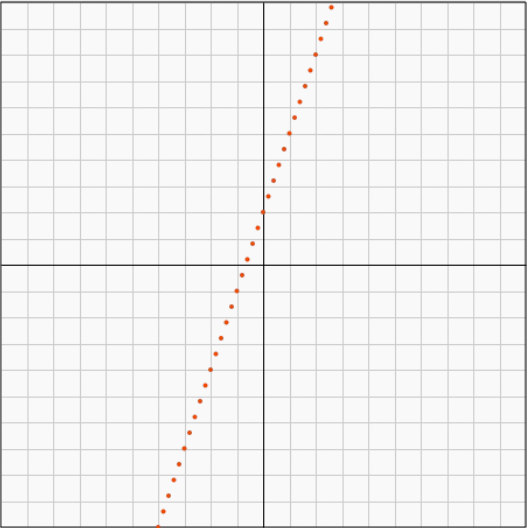
\includegraphics[scale=0.3]{images/trace_3x2_graph1.png}
\caption{Graphique affiché avec nb\_points = 100}
\end{figure}
\begin{figure}[H]
\centering
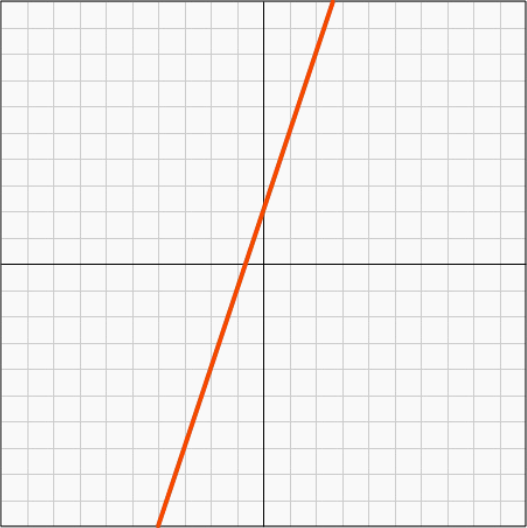
\includegraphics[scale=0.3]{images/trace_3x2_graph2.png}
\caption{Graphique affiché avec nb\_points = 100}
\end{figure}
\end{exemple}
\section{Algorithmes simples}
On cherche tout d'abord à calculer l'image par une fonction $f$ donnée d'un réel $x$ donné. Le code à écrire est alors 
\begin{algobox}
\Variables
\Ligne x EST\_DU\_TYPE NOMBRE
\Ligne y EST\_DU\_TYPE NOMBRE
\DebutAlgo
\Ligne SAISIR x
\Ligne y PREND\_LA\_VALEUR f(x)
\Ligne AFFICHER y
\FinAlgo
\end{algobox}
Par exemple si $f:x\mapsto3x+2$, on écrit le code
\begin{algobox}
\Variables
\Ligne x EST\_DU\_TYPE NOMBRE
\Ligne y EST\_DU\_TYPE NOMBRE
\DebutAlgo
\Ligne SAISIR x
\Ligne y PREND\_LA\_VALEUR 3*x+2
\Ligne AFFICHER y
\FinAlgo
\end{algobox}
\section{Activités algorithmique}
Toutes les activités algorithmiques du cours de 1ère S sont regroupés ici.
\subsection{Trinôme du second degré}
On aimerait calculer l'image par un trinôme $f:x\mapsto ax^2+bx+c$, d'un réel $x$. Le code est alors
\begin{algobox}
\Variables
\Ligne x EST\_DU\_TYPE NOMBRE
\Ligne y EST\_DU\_TYPE NOMBRE
\Ligne a EST\_DU\_TYPE NOMBRE
\Ligne b EST\_DU\_TYPE NOMBRE
\Ligne c EST\_DU\_TYPE NOMBRE
\DebutAlgo
\Ligne SAISIR a
\Ligne SAISIR b
\Ligne SAISIR c
\Ligne //Le trinome est maintenant défini
\Ligne SAISIR x
\Ligne y PREND\_LA\_VALEUR a*x*x + b*x + c
\Ligne AFFICHER y
\FinAlgo
\end{algobox}
Par exemple, $a=1$, $b=3$ et $c=-4$ ainsi que $x=2$, l'algorithme affiche $6$\newline

On veut maintenant calculer les racines d'un trinôme. On va avoir besoin d'une structure en Si....Alors pour différencier les cas avec le discriminant. La première étape de l'algorithme (après que l'on ait rentré les coefficients $a,b,c$ du trinôme) est de calculer le discriminant. Ensuite on utilise deux Si...Alors... Sinon : 
\begin{algobox}
\Variables
\Ligne x EST\_DU\_TYPE NOMBRE
\Ligne y EST\_DU\_TYPE NOMBRE
\Ligne a EST\_DU\_TYPE NOMBRE
\Ligne b EST\_DU\_TYPE NOMBRE
\Ligne c EST\_DU\_TYPE NOMBRE
\Ligne Delta EST\_DU\_TYPE NOMBRE
\DebutAlgo
\Ligne SAISIR a
\Ligne SAISIR b
\Ligne SAISIR c
\Ligne //Le trinome est maintenant défini
\Ligne Delta PREND\_LA\_VALEUR b*b - 4*a*c
\Si{(Delta > 0)}
\DebutSi
\Ligne x PREND\_LA\_VALEUR (-b + sqrt(Delta))/(2*a)
\Ligne y PREND\_LA\_VALEUR (-b-sqrt(Delta))/(2*a)
\Ligne AFFICHER x
\Ligne AFFICHER y
\FinSi
\Sinon
\DebutSinon
\Si{(Delta = 0)}
\DebutSi
\Ligne x PREND\_LA\_VALEUR -b/(2*a)
\Ligne AFFICHER x
\FinSi
\Sinon
\DebutSinon
\Ligne AFFICHER "Le trinôme n'a pas de racines réelles"
\FinSinon
\FinSinon
\FinAlgo

\end{algobox}
On peut aussi écrire un algorithme qui va permettre de tracer la courbe représentative d'un trinôme en s'inspirant du travail sur la boucle POUR DE A 

\begin{algobox}
\Variables
\Ligne a EST\_DU\_TYPE NOMBRE
\Ligne b EST\_DU\_TYPE NOMBRE
\Ligne c EST\_DU\_TYPE NOMBRE
\Ligne xmin EST\_DU\_TYPE NOMBRE
\Ligne xmax EST\_DU\_TYPE NOMBRE
\Ligne nb\_points EST\_DU\_TYPE NOMBRE
\Ligne pas EST\_DU\_TYPE NOMBRE
\Ligne k EST\_DU\_TYPE NOMBRE
\Ligne x EST\_DU\_TYPE NOMBRE
\DebutAlgo
\Ligne SAISIR a
\Ligne SAISIR b
\Ligne SAISIR c
\Ligne //le trinôme est défini
\Ligne SAISIR xmin
\Ligne SAISIR xmax
\Ligne SAISIR nb\_points
\Ligne pas PREND\_LA\_VALEUR (xmax-xmin)/nb\_points
\Pour{k}{0}{nb\_points}
\DebutPour
\Ligne x PREND\_LA\_VALEUR xmin + k*pas
\Ligne TRACER\_POINT (x,a*x*x+b*x+c)
\FinPour
\FinAlgo

\end{algobox}
Par exemple
\begin{verbatim}
> // Application de l'algorithme
> 
> // Début algorithme
> a = 1
> b = -1
> c = -1
> xmin = -10
> xmax = 10
> nb\_points = 1000
\end{verbatim}
on obtient, sur le graphique
\begin{figure}[H]
\centering
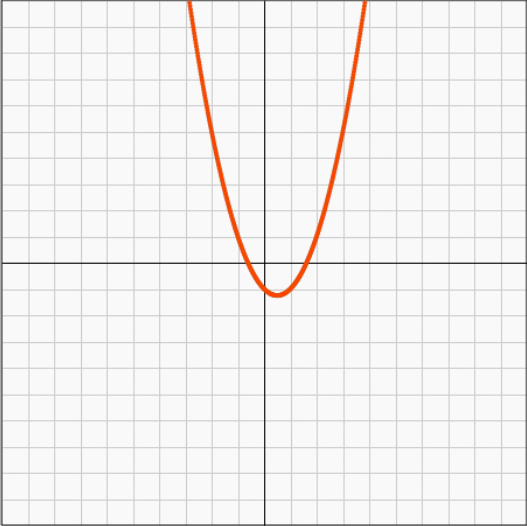
\includegraphics[scale=0.3]{images/trace_trinome_xx_-x_-1.png}
\caption{Graphique affiché}
\end{figure}
\subsection{Fonctions de références}
Pas de demande particulière du programme. On peut utiliser l'algorithme de trace de fonction pour représenter les fonctions de références
\subsection{Dérivation}
Pas de demande particulière du programme.
\subsection{Suites}
On peut écrire un algorithme pour calculer (et afficher) les $N$ premiers termes d'une suite $u_n$ définie par $u_n = f(n)$ où $f$ est une fonction connue : 

\begin{algobox}
\Variables
\Ligne k EST\_DU\_TYPE NOMBRE
\Ligne N EST\_DU\_TYPE NOMBRE
\DebutAlgo
\Ligne SAISIR N
\Pour{k}{0}{N-1}
\DebutPour
\Ligne AFFICHERCALCUL f(k)
\Ligne TRACER\_POINT (k,f(k))
\FinPour
\FinAlgo

\end{algobox}
On peut aussi écrire un algorithme qui permet de calculer (et d'afficher) les $N$ premiers termes d'une suite $u_n$ définie par $u_0$ et $u_{n+1} = f(u_n)$ où $f$ est une fonction connue
\begin{algobox}
\Variables
\Ligne k EST\_DU\_TYPE NOMBRE
\Ligne N EST\_DU\_TYPE NOMBRE
\Ligne u EST\_DU\_TYPE NOMBRE
\Ligne u0 EST\_DU\_TYPE NOMBRE
\DebutAlgo
\Ligne SAISIR N
\Ligne SAISIR u0
\Ligne u PREND\_LA\_VALEUR u0
\Pour{k}{0}{N-1}
\DebutPour
\Ligne u u PREND\_LA\_VALEUR f(u)
\Ligne AFFICHER u
\Ligne TRACER\_POINT (k,f(k))
\FinPour
\FinAlgo

\end{algobox}
Par exemple, on peut particulariser cet algorithme dans le cas où $u$ est la suite géométrique de raison $q$ et de premier terme $u_0$ : 
\begin{algobox}
\Variables
\Ligne k EST\_DU\_TYPE NOMBRE
\Ligne N EST\_DU\_TYPE NOMBRE
\Ligne u EST\_DU\_TYPE NOMBRE
\Ligne u0 EST\_DU\_TYPE NOMBRE
\Ligne q EST\_DU\_TYPE NOMBRE
\DebutAlgo
\Ligne SAISIR N
\Ligne SAISIR u0
\Ligne SAISIR q
\Ligne u PREND\_LA\_VALEUR u0
\Pour{k}{0}{N-1}
\DebutPour
\Ligne u u PREND\_LA\_VALEUR q*u
\Ligne AFFICHER u
\Ligne TRACER\_POINT (k,f(k))
\FinPour
\FinAlgo
\end{algobox}

On se donne maintenant une suite croissante non majorée (qui tend donc vers l'infini) et on aimerait connaitre le rang $N$ à parti duquel $\forall n \geq N $, $u_n \geq A$, $A$ étant donné
\begin{algobox}
\Variables
\Ligne N EST\_DU\_TYPE NOMBRE
\Ligne u EST\_DU\_TYPE NOMBRE
\Ligne A EST\_DU\_TYPE NOMBRE
\DebutAlgo
\Ligne SAISIR A
\Ligne N PREND\_LA\_VALEUR 0
\Ligne u PREND\_LA\_VALEUR f(N)
\Tantque{(u < A)}
\DebutTantQue
\Ligne N PREND\_LA\_VALEUR N+1
\Ligne u PREND\_LA\_VALEUR f(N)
\FinTantQue
\Ligne AFFICHER N
\FinAlgo

\end{algobox}
\begin{verbatim}
> // Application de l'algorithme
> On prend $f(n) = 3*\sqrt{n}+2$
>
> // Début de l'algorithme
> A = 100
> 1068
\end{verbatim}
On remarque que $3 \times \sqrt{1067} +2 \simeq 99,99489$ et $3 \times \sqrt{1068} +2 \simeq 100,0408$

On peut évidemment adapter l'algorithme précédent pour des suites définies par récurrence.
\subsection{Géométrie plane}
Quelques algorithmes sur la géométrie plane\newline

Déterminer si deux vecteurs $\covec{x_1}{y_1}$ et $\covec{x_2}{y_2}$ sont colinéaires.
\begin{algobox}
\Variables
\Ligne x1 EST\_DU\_TYPE NOMBRE
\Ligne y1 EST\_DU\_TYPE NOMBRE
\Ligne x2 EST\_DU\_TYPE NOMBRE
\Ligne y2 EST\_DU\_TYPE NOMBRE
\DebutAlgo
\Ligne SAISIR x1
\Ligne SAISIR y1
\Ligne SAISIR x2
\Ligne SAISIR y2
\Si{(x1*y2-x2*y1 = 0)}
\DebutSi
\Ligne AFFICHER "Les vecteurs sont colinéaires"
\FinSi
\Sinon
\DebutSinon
\Ligne AFFICHER "Les vecteurs ne sont pas colinéaires"
\FinSinon
\FinAlgo
\end{algobox}
\begin{verbatim}
> // Application de l'algorithme
>
> // Début de l'algorithme
> x1 = 1
> y1 = 0
> x2 = 0
> y2 = 1 
> "Les vecteurs ne sont pas colinéaires"
>
> // Début de l'algorithme
> x1 = 2
> y1 = 3
> x2 = 4
> y2 = 6 
> "Les vecteurs ne sont colinéaires"
\end{verbatim}

On aimerait connaitre une équation cartésienne de droite passant par les points $A(xA,yA)$ et $B(xB,yB)$ ($A$ et $B$ distincts). On détermine (sauf si la droite est parallèle à l'axe ds ordonnées) l'équation réduite de la droite.
\begin{algobox}
\Variables
\Ligne xA EST\_DU\_TYPE NOMBRE
\Ligne yA EST\_DU\_TYPE NOMBRE
\Ligne xB EST\_DU\_TYPE NOMBRE
\Ligne coeff\_dir EST\_DU\_TYPE NOMBRE
\Ligne ord\_org EST\_DU\_TYPE NOMBRE
\Ligne res EST\_DU\_TYPE CHAINE
\Ligne yB EST\_DU\_TYPE NOMBRE
\DebutAlgo
\Ligne SAISIR xA
\Ligne SAISIR yA
\Ligne SAISIR xB
\Ligne SAISIR yB
\Si{(xA = xB)}
\DebutSi
\Ligne //Cas où la droite est parallèle à l'axe des ordonnées
\Ligne res PREND\_LA\_VALEUR "L'équation cartésienne de droite est y = " + xA.toString()
\Ligne AFFICHER res
\FinSi
\Sinon
\DebutSinon
\Ligne coeff\_dir PREND\_LA\_VALEUR (yB-yA)/(xB-xA)
\Ligne ord\_org PREND\_LA\_VALEUR yA-xA*coeff\_dir
\Ligne res PREND\_LA\_VALEUR "L'équation cartésienne de la droite est y = " + coeff\_dir.toString() + "x+" + ord\_org.toString()
\Ligne AFFICHER res
\FinSinon
\FinAlgo
\end{algobox}
\begin{verbatim}
> // Application de l'algorithme
>
> // Début de l'algorithme
> xA = 1
> yA = 0
> xB = 1
> yB = 2
> "L'équation cartésienne de droite est y = 1"
>
> xA = 0
> yA = 1
> xB = 1
> yB = 3
> "L'équation cartésienne de la droite est y = 2x+1"
\end{verbatim}
Petite précision sur l'instruction toSring : si x est une variable de type nombre alors x.toString est la variable de type chaine qui représente le nombre x.
\subsection{Trigonométrie}
On va tracer les fonctions $x\mapsto \sin(x)$ et $x\mapsto \cos(x)$ grâce à l'algorithme de trace
\begin{algobox}
\Variables
\Ligne xmin EST\_DU\_TYPE NOMBRE
\Ligne xmax EST\_DU\_TYPE NOMBRE
\Ligne nb\_points EST\_DU\_TYPE NOMBRE
\Ligne pas EST\_DU\_TYPE NOMBRE
\Ligne k EST\_DU\_TYPE NOMBRE
\Ligne x EST\_DU\_TYPE NOMBRE
\DebutAlgo
\Ligne SAISIR xmin
\Ligne SAISIR xmax
\Ligne SAISIR nb\_points
\Ligne pas PREND\_LA\_VALEUR (xmax-xmin)/nb\_points
\Pour{k}{0}{nb\_points}
\DebutPour
\Ligne x PREND\_LA\_VALEUR xmin + k*pas
\Ligne TRACER\_POINT [rouge] (x,cos(x))
\Ligne TRACER\_POINT [bleu] (x,sin(x))
\FinPour
\FinAlgo
\end{algobox}
\begin{figure}[H]
\centering
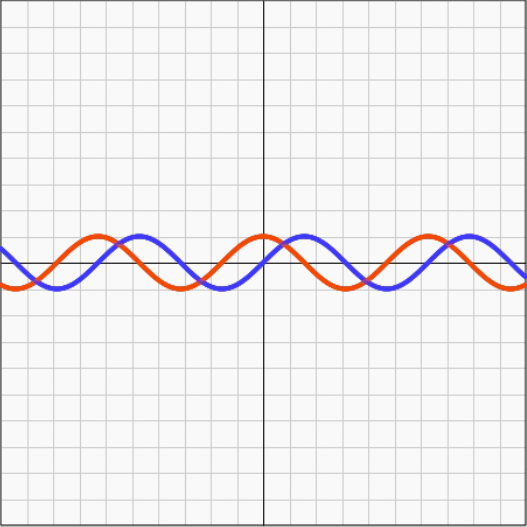
\includegraphics[scale=0.5]{images/cos_sin.png}
\caption{Courbes représentatives des fonctions sinus et cosinus tracées grâce à l'algorithme}
\end{figure}
Tracer maintenant le cercle trigonométrique à l'aide des fonctions cosinus et sinus : 
\begin{algobox}
\Variables
\Ligne xmin EST\_DU\_TYPE NOMBRE
\Ligne xmax EST\_DU\_TYPE NOMBRE
\Ligne nb\_points EST\_DU\_TYPE NOMBRE
\Ligne pas EST\_DU\_TYPE NOMBRE
\Ligne k EST\_DU\_TYPE NOMBRE
\Ligne x EST\_DU\_TYPE NOMBRE
\DebutAlgo
\Ligne SAISIR xmin
\Ligne SAISIR xmax
\Ligne SAISIR nb\_points
\Ligne pas PREND\_LA\_VALEUR (xmax-xmin)/nb\_points
\Pour{k}{0}{nb\_points}
\DebutPour
\Ligne x PREND\_LA\_VALEUR xmin + k*pas
\Ligne TRACER\_POINT (cos(x),sin(x))
\FinPour
\FinAlgo

\end{algobox}
Ainsi en appelant la fonction avec pour paramètre xmin = 0, xmax = 7 (en fait, xmax = 2$\pi$ suffit) et nb\_points = 500, on obtient, 
\begin{figure}[H]
\centering
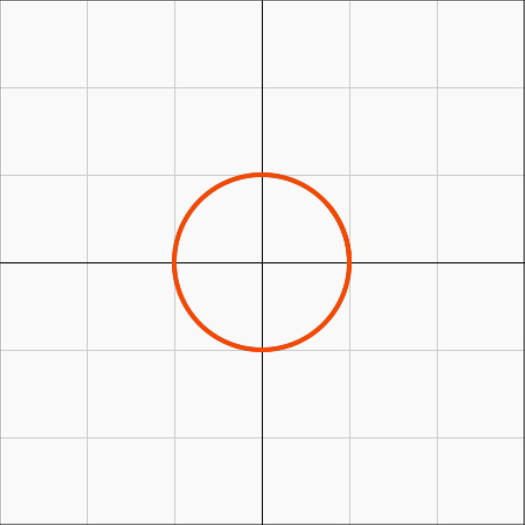
\includegraphics[scale=0.5]{images/cercle_trigo.png}
\caption{Cercle de centre 0 et de rayon 1 tracé à l'aide de l'algorithme}
\end{figure}
\subsection{Produit scalaire}
On peut écrire un algorithme tout simple qui calcule le produit scalaire
\begin{algobox}
\Variables
\Ligne xA EST\_DU\_TYPE NOMBRE
\Ligne yA EST\_DU\_TYPE NOMBRE
\Ligne xB EST\_DU\_TYPE NOMBRE
\Ligne yB EST\_DU\_TYPE NOMBRE
\DebutAlgo
\Ligne SAISIR xA
\Ligne SAISIR yA
\Ligne SAISIR xB
\Ligne SAISIR yB
\Ligne AFFICHERCALCUL xA*xB+yA*yB
\FinAlgo
\end{algobox}
\begin{verbatim}
> // Application de l'algorithme
>
> xA = 2; yA = -1; xB = 1; yB = 3
> -1
\end{verbatim}
Ecrivons maintenant un algorithme qui nous dit si deux vecteurs sont orthogonaux
\begin{algobox}
\Variables
\Ligne xA EST\_DU\_TYPE NOMBRE
\Ligne yA EST\_DU\_TYPE NOMBRE
\Ligne xB EST\_DU\_TYPE NOMBRE
\Ligne yB EST\_DU\_TYPE NOMBRE
\DebutAlgo
\Ligne SAISIR xA
\Ligne SAISIR yA
\Ligne SAISIR xB
\Ligne SAISIR yB
\Si{(xA*xB+yA*yB == 0)}
\DebutSi
\Ligne AFFICHER "Les vecteurs sont orthogonaux"
\FinSi
\Sinon
\DebutSinon
\Ligne AFFICHER "Les vecteurs ne sont pas orthogonaux"
\FinSinon
\FinAlgo
\end{algobox}
\begin{verbatim}
> // Application de l'algorithme
>
> xA = 1; yA = 0; xB = 0; yB = 1
> "Les vecteurs sont orthogonaux"
> 
> xA = 2; yA = -1; xB = 1; yB = 3
> "Les vecteurs ne sont pas orthogonaux"
\end{verbatim}
\subsection{Statistiques et probabilités}
Certains algorithmes seront à réaliser dans les sujets : pour les découvrir, regarder la correction
\chapter{Raisonnements ensemblistes}
\label{chap:ensembles}
\section{Ensembles}
\defi{ : ensemble}{Un ensemble est une collection d'objets mathématiques. Les objets sont appelés les éléments de l'ensemble}\newline

\begin{exemple}
$$A = \{\pi, 4, \sqrt{2}\}$$
est un ensemble. On peut aussi avoir des ensembles de fonctions : 
$$B = \left\{x\mapsto x^2,x\mapsto \sin(x),x\mapsto \dfrac{1}{\sqrt{x}}\right\}$$
voire des ensembles qui mixent les deux 
$$C = \{3,x\mapsto x\}$$
\end{exemple}
\defi{ : ensembles égaux}{On dit que 2 ensembles $A$ et $B$ sont égaux s'ils ont les mêmes éléments. On note alors $A = B$}\newline

\defi{ : ensembles usuels}{Les ensembles suivants sont souvent utilisés : \begin{itemize}\item L'ensemble vide $\varnothing$ $$\varnothing = \{\}$$ \item L'ensemble des entiers naturels $\N$ $$\N = \{0,1,2,3,\ldots\}$$\item L'ensemble des entiers relatifs $\Z$ $$\Z = \{\ldots,-3,-2,-1,0,1,2,3,\ldots\}$$ \item L'ensemble des entiers décimaux $\mathbb{D}$, c'est à dire l'ensembles des nombres qui s'écrivent $\dfrac{a}{10^n}$ avec $a\in\Z$ et $n\in \Z$ \item L'ensembles des rationnels $\Q$, c'est à dire des nombres qui s'écrivent $\dfrac{p}{q}$ avec $p\in \Z$, $q\in \N^*$ et $pgcd(p,q)=1$ \item L'ensemble des réels $\R$\end{itemize}}\newline

\defi{ : signleton}{On appelle singleton un ensemble composé d'un seul élément}\newline

\defi{ : quelques notations}{Soit $A\subset \R$. On note $$A_{+} = \{x\in A / x\geq 0\} $$ $$A_{-} = \{x\in A / x\leq 0\}$$ $$A^* = \{x\in A / x\neq 0\} = A\backslash \{0\}$$}
\section{Appartenance}
\defi{ : appartenance}{Soit $A$ un ensemble et $a$ un objet mathématique. Si $a$ est un élément de $A$ on dit que $a$ appartient à $A$ et on note $a\in A$}\newline

\begin{exemple}
On a 
$$3\in \Z$$
$$\dfrac{2}{3} \in \Q$$
$$\pi \notin \Q$$
\end{exemple}
\section{Inclusion}
\defi{ : inclusion}{Soient $A$ et $B$ deux ensembles. Si tous les éléments de $A$ sont aussi des éléments de $B$, alors ont dit que $A$ est inclus dans $B$ et on note $A \subset B$}\newline

Autrement dit 
$$A \subset B \Leftrightarrow \forall x \in A, x\in B$$
ou encore
$$A \subset B \Leftrightarrow (x\in A \Rightarrow x\in B)$$

\begin{exemple}
$$\N \subset \Z \subset \mathbb{D} \subset \Q \subset \R$$
\end{exemple}

\methode{pour montrer que $A\subset B$}{\begin{enumerate}\item Considérer un élément $x$ de $A$ \item Montrer que $x \in B$ (pour cela utiliser des propriétés relatives à $A$)  \end{enumerate}}\newline

\begin{exemple}
On note 
$$A = \{4\times k / k\in \Z\}$$
$$B = \{2\times k / k\in \Z\}$$
($A$ ensemble des multiples de 4 et $B$ ensemble des multiples de 2)\newline
Montrer $A \subset B$\newline

Soit $x\in A$\newline
Il existe $k\in \Z$ tel que $x = 4\times k$. Alors $x = 2\times (2k)$ et $2k \in \Z$ donc $x\in B$. On déduit $A\subset B$
\end{exemple}

\defi{ : inclusion stricte}{Si on a $A\subset B$ et $A\neq B$, alors on dit qu'il ya inclusion stricte de $A$ dans $B$ et on note parfois $A\varsubsetneq B$}\newline


\propriete{}{Pour tout ensemble $A$, $$\varnothing \subset A$$ et $$A\subset A$$}\newline

\begin{preuve}
Y a-t-il vraiment quelque chose à prouver ?
\end{preuve}

\prop{ : double inclusion}{Soient $A$ et $B$ deux ensembles. Si $A \subset B$ et si $B \subset A$ alors $A = B$}\newline

\begin{preuve}
\underline{1ère preuve}\newline
Tout élément de $A$ est aussi un élément de $B$\newline
Tout élément de $B$ est aussi un élément de $A$\newline
$A$ et $B$ ont donc les mêmes éléments et sont par conséquents égaux\newline

\underline{2ème preuve}\newline
Supposons par l'absurde $A\neq B$
1er cas : il existe un élément $x$ de $A$ tel que $x\notin B$ : contradiction avec $A \subset B$\newline
2ème cas : il existe un élément $x$ de $B$ tel que $x\notin A$ : contradiction avec $B \subset A$\newline
On obtient une contradiction dans les deux cas donc on a bien $A = B$
\end{preuve}
\methode{pour prouver que deux ensembles $A$ et $B$ sont égaux à l'aide de la double inclusion}{\begin{enumerate}\item Montrer que $A\subset B$ \item Montrer que $B\subset A$ \item En déduire $A = B$ \end{enumerate}}
\section{Différence}
\defi{ : différence de 2 ensembles}{Soient $A$ et $B$ deux ensembles. On note $A\backslash B$ l'ensemble constitué des éléments de $A$ qui ne sont pas dans $B$}\newline

\begin{exemple}
$$\{3,2,0\} \backslash \{2\} = \{3,0\}$$
\end{exemple}
\begin{figure}[H]
\centering
\begin{tikzpicture}
\begin{scope}[even odd rule]
\clip (3,0) circle (2) (-3,-3) rectangle (3,3);
\fill [cyan!60]  (0,0) circle (2);
\end{scope}
\draw (0,0) circle (2);
\draw (3,0) circle (2);
\node at (0,0) {$A$};
\node at (3,0) {$B$};
\end{tikzpicture}
\caption{Diagramme représentant $A\backslash B$ en bleu}
\end{figure}
\section{Réunion}
\defi{ : réunion de deux ensembles}{Soit $A$ et $B$ deux ensembles. On appelle réunion de $A$ et de $B$ et on note $A\cup B$ l'ensemble constitué des éléments de $A$ et des éléments de $B$ réunis}\newline

\begin{exemple}
Si $$A = \{2,8,-3,4\}$$ et $$B = \{1,0,4\}$$ alors $$A\cup B= \{2,8,-3,4,1,0\}$$
\end{exemple}
\begin{figure}[H]
\centering
\begin{tikzpicture}
\draw [fill=cyan!60] (0,0) circle (2);
\draw [fill=cyan!60]  (3,0) circle (2);
\draw (0,0) circle (2);
\node at (0,0) {$A$};
\node at (3,0) {$B$};
\end{tikzpicture}
\caption{Diagramme représentant $A\cup B$ en bleu}
\end{figure}

On a 
$$x\in A\cup B \Leftrightarrow x\in A \text{ ou } x\in B$$
\defi{ : réunion de plusieurs ensembles}{Soit $A_1, A_2,\ldots,A_n$ $n$ ensembles. On appelle réunion de $A_1,A_2,\ldots,A_n$ et on note $\displaystyle \bigcup_{k=0}^n A_k$ $$\bigcup_{k=0}^n A_k = A_1 \cup A_2 \cup \ldots \cup A_n$$ }\newline

\propriete{}{Soient $A$ et $B$ deux ensembles. Alors $$A \subset A\cup B$$ $$B \subset A\cup B$$}\newline

\begin{preuve}
Par définition, les éléments de $A$ sont dans $A\cup B$ et de même pour les éléments de $B$
\end{preuve}

\propriete{}{Soit $A,B,C$ trois ensembles. On suppose $B\subset A$ et $C \subset A$. Alors $$B\cup C \subset A$$}\newline

\begin{preuve}
Tous les éléments de $B$ et $C$ étant aussi des éléments de $A$, quand on les réunit, bah ça reste tous des éléments de $A$...
\end{preuve}

\propriete{}{Soient $A$ et $B$ deux ensembles tels que $A \subset B$. Alors $$A\cup B =B$$}\newline
\section{Intersection}
\defi{ : intersection de deux ensembles}{Soit $A$ et $B$ deux ensembles. On appelle intersection de $A$ et de $B$ et on note $A\cap B$ l'ensemble constitué des éléments communs à $A$ et à $B$}\newline

\begin{exemple}
Si $$A = \{2,8,-3,4\}$$ et $$B = \{1,0,4\}$$ alors $$A\cap B= \{4\}$$
\end{exemple}
\begin{figure}[H]
\centering
\begin{tikzpicture}
\begin{scope}
\clip (0,0) circle (2);
\fill [cyan!60]  (3,0) circle (2);
\end{scope}
\draw (0,0) circle (2);
\draw (3,0) circle (2);
\node at (0,0) {$A$};
\node at (3,0) {$B$};
\end{tikzpicture}
\caption{Diagramme représentant $A\cap B$ en bleu}
\end{figure}

On a 
$$x\in A\cap B \Leftrightarrow x\in A \text{ et } x\in B$$
\defi{ : intersection de plusieurs ensembles}{Soit $A_1, A_2,\ldots,A_n$ $n$ ensembles. On appelle réunion de $A_1,A_2,\ldots,A_n$ et on note $\displaystyle \bigcap_{k=0}^n A_k$ $$\bigcap_{k=0}^n A_k = A_1 \cap A_2 \cap \ldots \cap A_n$$ }\newline

\propriete{}{Soient $A$ et $B$ deux ensembles. Alors $$A\cap B \subset A$$ $$A\cap B \subset B$$}\newline

\begin{preuve}
Par définition, les éléments de $A\cap B$ sont à la fois dans $A$ et dans $B$ d'où le résultat
\end{preuve}

\propriete{}{Soit $A,B,C$ trois ensembles. On suppose $A\subset B$ et $A \subset C$. Alors $$A \subset B\cap C$$}\newline

\begin{preuve}
Soit $x\in A$\newline
$A\subset B$ donc $x\in B$\newline
$A \subset C$ donc $x\in C$\newline
$x \in B$ et $x\in C$ donc $x\in A\cap B$\newline

Ainsi 
$$A \subset B\cap C$$
\end{preuve}
\propriete{}{Soient $A$ et $B$ deux ensembles tels que $A \subset B$. Alors $$A\cap B =A$$}\newline


\defi{ : ensembles disjoints}{Ont dit que 2 ensembles $A$ et $B$ sont disjoints lorsque $$A\cap B = \varnothing$$}
\section{Distributivité}
\propriete{}{Soient $A,B,C$ trois ensembles, alors $$A \cap (B\cup C) = (A\cap B)\cup (A\cap C)$$}\newline

\begin{preuve}
On peut faire une preuve "à voix haute" mais on va ici raisonner par double inclusion : \newline


\underline{$A \cap (B\cup C) \subset (A\cap B)\cup (A\cap C)$}\newline
Soit $x \in A \cap (B\cup C)$. On a alors $x\in A$. On a de plus $x\in B$ ou (non exclusif) $x\in C$. Ainsi on a ($x\in A$ et $x\in B$) ou (non exclusif) ($x \in A$ et $x\in C$) donc $x\in (A\cap B)\cup (A\cap C)$\newline

\underline{$(A\cap B)\cup (A\cap C) \subset A \cap (B\cup C)$}\newline
Soit $x \in (A\cap B)\cup (A\cap C)$. On a ($x\in A$ et $x\in B$) ou (non exclusif) ($x\in A$ et $x \in C$). Ainsi $x\in A$ et ($x\in B$ ou (non exclusif) $x\in C$) donc $x\in A \cap (B\cup C)$\newline

Ainsi 
$$A \cap (B\cup C) = (A\cap B)\cup (A\cap C)$$
\end{preuve}

\propriete{}{Soient $A,B,C$ trois ensembles, alors $$A \cup (B\cap C) = (A\cup B)\cap (A\cup C)$$}\newline

\begin{preuve}
La preuve est la même (presque !) que précédemment
\end{preuve}
\section{Complémentaire}
\defi{ : complémentaire par rapport à un ensemble}{Soit $E$ un ensemble et $A \subset E$. On appelle complémentaire de $A$ par rapport à $E$ (ou dans $E$) et on note $\complement_E A$ (ou s'il n'a pas ambiguïté $\overline{A}$) l'ensemble $$\overline{A} = E \backslash A$$}\newline

On rencontre parfois d'autres notations, comme 
$$\complement_E^A, ^\complement A, A^\complement$$

\begin{exemple}
Le complémentaire de $\{\pi,\sqrt{2},6,18,3\}$ par rapport à $\{14,\pi,5\sqrt{2},6,18,\sqrt{5},3\}$ est $\{14,5,\sqrt{5}\}$
\end{exemple}
\begin{figure}[H]
\centering
\begin{tikzpicture}
\draw [fill=yellow!60] (-5,-3) rectangle (5,3);
\draw [fill=cyan!60] (0,0) circle (2);
\node at (0,0) {$A$};
\node at (5,3) [right] {$E$};
\end{tikzpicture}
\caption{Diagramme représentant $A$ en bleu et son complémentaire $\overline{A}$ en jaune}
\end{figure}

Dans la suite de cette partie, on considère $E$ un ensemble, et on fait les complémentaires par rapport à cet ensemble. \newline

\propriete{}{On a $$\overline{E} = \varnothing$$ $$ \overline{\varnothing} = E$$}\newline

On a même équivalence : 
$$\overline{A} = \varnothing \Leftrightarrow A = E$$
$$\overline{A} = E \Leftrightarrow A = \varnothing$$

\propriete{ : caractérisation}{Soit $A \subset E$. Alors $$x \in A \Leftrightarrow x\notin \overline{A}$$ $$x\in \overline{A} \Leftrightarrow x\notin A$$}\newline


\propriete{}{Soit $A \subset E$. Alors $\overline{A} \subset E$}\newline

\begin{preuve}
Par définition, $\overline{A}$ es l'ensemble des éléments de $E$ privés de ceux de $A$ donc $\overline{A} \subset E$ 
\end{preuve}

\propriete{}{Soit $A \subset E$. Alors les ensembles $A$ et $\overline{A}$ sont disjoints ($A \cap \overline{A} = \varnothing$)}\newline

\begin{preuve}
En effet, appartenir à $A \cap \overline{A}$ revient à appartenir à $A$ et ne pas appartenir à $A$ : cet ensemble ne peut être que vide
\end{preuve}

\propriete{}{Soit $A \subset E$. Alors $$A \cup \overline{A} = E$$}\newline

\begin{preuve}
On a $A \subset E$ et $\overline{A} \subset E$ donc $A\cup \overline{A} \subset E$\newline

Soit $x\in E$. Si $x\in A$ bah $x\in A$ et si $x\notin A$ alors $x\in \overline{A}$ donc $E \subset A\cup \overline{A}$\newline

Finalement $$E = A \cup \overline{A}$$
\end{preuve}

\propriete{}{Soit $A\subset E$. Alors $$\overline{\overline{A}}=A$$}\newline

\begin{preuve}
$$x\in A \Leftrightarrow x \notin \overline{A} \Leftrightarrow x \in \overline{\overline{A}}$$
(d'après la caractérisation), d'où l'égalité
\end{preuve}
\section{Lois de Morgan}
On considère un ensemble $E$ pour les complémentaires \newline


\theo{ : lois de Morgan}{Soient $A\subset E$ et $B\subset E$. Alors $$\overline{A\cup B} = \overline{A}\cap \overline{B}$$ $$\overline{A\cap B} = \overline{A}\cup \overline{B}$$}\newline

\begin{preuve}
\underline{1ère égalité}\newline

Soit $x \in \overline{A\cup B}$. Alors $x \notin A\cup B$. On en déduit que $x\notin A$ et $x\notin B$. Donc $x\in \overline{A}$ et $x\in \overline{B}$ d'ou finalement $x\in \overline{A}\cap \overline{B}$\newline
Ainsi 
$$\overline{A\cup B} \subset \overline{A}\cap \overline{B}$$

Soit $x\in \overline{A}\cap \overline{B}$. Alors $x\in \overline{A}$ et $x\in \overline{B}$ donc $x\notin A$ et $x \notin B$. Ainsi $x\notin A\cup B$ donc $x\in \overline{A \cup B}$\newline
Ainsi 
$$\overline{A}\cap \overline{B} \subset \overline{A\cup B}$$
On déduit finalement 
$$\overline{A\cup B} = \overline{A}\cap \overline{B}$$
(par double inclusion)\newline


\underline{2ème égalité}\newline
Elle se déduit en fait de la première : on applique la première égalité non à $A$ et $B$ mais à $\overline{A}$ et $\overline{B}$ : 
$$\overline{\overline{A}\cup \overline{B}} = \overline{\overline{A}}\cap \overline{\overline{B}}$$
$$\overline{\overline{A}\cup \overline{B}} = A\cap B$$
d'où en passant des 2 côtés au complémentaire
$$\overline{\overline{\overline{A}\cup \overline{B}}} = \overline{A\cap B}$$
$$\overline{A}\cup \overline{B} = \overline{A\cap B}$$
\end{preuve}
\section{Cardinal}
\defi{ : cardinal}{Soit $A$ un ensemble. S'il possède un nombre fini d'élément, on appelle cardinal de $A$ et on note $\text{Card}(A)$ le nombre d'éléments de $A$}\newline
\begin{exemple}
$$\text{Card}(\{-1,8,6,\pi\}) = 4$$
$$\text{Card}([\![1,n]\!]) = n$$
$$\text{Card}([\![0,n]\!]) = n+1$$
\end{exemple}
\prop{ : cardinal d'un complémentaire}{Soit $E$ un ensemble et $A\subset E$. Alors $$\text{Card}(\overline{A}) = \text{Card}(E) - \text{Card}(A)$$}\newline

\begin{remarque}
Formule analogue à 
$$P(\overline{A}) = 1 - P(A)$$
($1 = P(\Omega)$)
\end{remarque}

\prop{ : cardinal d'une réunion}{Soient $A$ et $B$ deux ensembles. Alors $$\text{Card}(A\cup B) = \text{Card}(A) + \text{Card}(B) - \text{Card}(A\cap B)$$}\newline

\begin{remarque}
Analogue à la formule 
$$P(A\cup B) = P(A) + P(B) - P(A\cap B$$
\end{remarque}

\prop{ : cardinal d'une réunion disjointe}{Soient $A$ et $B$ deux ensembles disjoints. Alors $$\text{Card}(A\cup B) = \text{Card}(A) + \text{Card}(B)$$}\newline
\appendix
\part{Annexes}
\chapter{Notations}
\section*{Général}
\begin{itemize}
\item $\leftrightarrows$ : liens entre chapitres
\item \begin{prog} $\ldots$ \end{prog} : citation du programme
\item Si $a_1,a_2,\ldots,a_n$ sont des réels, on note $$\sum_{k=1}^n a_k = a_1+a_2+\ldots+a_n $$
\item Si $a_1,a_2,\ldots,a_n$ sont des réels, on note $$\prod_{k=1}^n a_k = a_1\times a_2\times \ldots\times a_n $$
\end{itemize}
\section*{Ensembles}
\begin{itemize}
\item Un ensemble est souvent noté en majuscule
\item On détaille les éléments d'un ensemble grâce à $\{$ et $\}$
\item Si $k$ et $n$ sont des entiers tels que $k\leq n$. On note $[\![k,n]\!] = \{k,k+1,\ldots,n\}$. Par exemple $[\![1,n]\!] = \{1,2,3,\ldots,n\}$
\item On utilise $\in$ pour signifier qu'un élément appartient à un ensemble
\item La réunion de deux ensembles est notée grâce à $\cup$
\item L'intersection de deux ensembles est notée grâce à $\cap$
\item Un nombre entier est habituellement notée $p$, $q$, $k$,...
\end{itemize}
\section*{Analyse}
\begin{itemize}
\item Une fonction est souvent notée $f$, $g$ ou $h$...
\item Le discriminant d'un trinôme est noté $\Delta$
\item L'ensemble de définition d'une fonction $f$ est noté $\mathscr{D}_f$
\item La courbe représentative d'une fonction $f$ est habituellement noté $\mathscr{C}_f$
\item Si $f$ est une fonction, on note $f'$ sa dérivée
\item Si $f$ et $g$ sont deux fonctions, on note $f+g$ la fonction qui à $x\mapsto f(x)+g(x)$
\item Si $f$ et $g$ sont deux fonctions, on note $f\times g$ la fonction qui à $x\mapsto f(x)\times g(x)$
\item Si $f$ et $g$ sont deux fonctions, on dit que $f \geq g$ lorsque pour tout $x$, $f(x) \geq g(x)$
\item Si $f$ est une fonction, on appelle zéros de $f$ les solutions de $f(x) = 0$
\item Les zéros d'un trinôme sont appelés racines d'un trinôme
\item La valeur absolue de $x$ est notée $|x|$
\item Une suite est habituellement notée $(u_n)$,$(v_n)$,$(w_n)$,...
\item La raison d'une suite arithmétique est habituellement notée $r$
\item La raison d'une suite géométrique est habituellement notée $q$
\end{itemize}
\section*{Géométrie}
\begin{itemize}
\item Un angle est habituellement noté $\alpha$, $\beta$, $\theta$,...
\item On désigne un vecteur par ses coordonnées $\vv{u} \covec{x}{y}$ ou $\vv{u} = \covec{x}{y}$
\item Le vecteur nul est noté $\vv{0}$
\item On utilise $\cdot$ pour désigner le produit scalaire : $\vv{u} \cdot \vv{v}$
\item On utilise $||\vv{u}||$ pour désigner la norme d'un vecteur $u$
\end{itemize}
\section*{Probabilités et statistiques}
\begin{itemize}
\item Une variable aléatoire est en général notée $X$, $Y$ ou $Z$...
\item Si $X$ est une variable aléatoire, alors on note $E(X)$ son espérance
\item Si $X$ est une variable aléatoire, alors on note $V(X)$ sa variance
\item Si $X$ est une variable aléatoire, alors on note $\sigma(X)$ son écart-type
\end{itemize}

\chapter{Logique mathématiques}
\emph{"En complément des objectifs rappelés ci-dessous, un travail sur la notion d'équivalence doit naturellement être mené en série scientifique (propriété caractéristique, raisonnement par équivalence)."}\newline

\emph{"Pour ce qui concerne le raisonnement logique, les élèves sont entraînés, sur des exemples, à :\begin{itemize}
\item utiliser correctement les connecteurs logiques "et", "ou" et à distinguer leur sens des sens courants de "et", "ou" dans le langage usuel ;
\item utiliser à bon escient les quantificateurs universel, existentiel (les symboles $\forall$, $\exists$ ne sont pas exigibles) et à repérer les quantifications implicites dans certaines propositions et, particulièrement, dans les propositions conditionnelles ;
\item distinguer, dans le cas d'une proposition conditionnelle, la proposition directe, sa réciproque, sa contraposée et sa négation ;
\item utiliser à bon escient les expressions "condition nécessaire", "condition suffisante" ;
\item formuler la négation d'une proposition ;
\item utiliser un contre-exemple pour infirmer une proposition universelle ;
\item reconnaître et utiliser des types de raisonnement spécifiques : raisonnement par disjonction des cas, recours à la contraposée, raisonnement par l'absurde.\end{itemize}}
\section{Enoncés, assertions, propriétés}
\defi{ : énoncé, assertion}{Un énoncé est une phrase portant sur des objets mathématiques. Un énoncé peut contenir une ou plusieurs variables libres, c'est à dire susceptibles d'êtres remplacées par des objets mathématiques. Un énoncé ne comportant aucun variable libre est appelée une assertion. Une assertion est susceptible d'avoir une valeur de vérité (vrai ou faux).}\newline


Lorsque dans un énoncé, toutes les variables libres sont remplacées par des objets mathématiques, on obtient une assertion.\newline

\begin{exemples}
\begin{enumerate}
\item $A : \text{"}3 \leq 2\text{"}$. $A$ est un assertion. Sa valeur de vérité est faux.
\item $$A(x) : \text{"}\sqrt{5} \leq x-4\text{"}$$ $A(x)$ est un énoncé avec une variable libre\newline

$$A(7) : \text{"} \sqrt{5} \leq 7 -4\text{"}$$ $A(7)$ est une assertion vraie
$$A(6) : \text{"} \sqrt{5} \leq 6 -4\text{"}$$ $A(6)$ est une assertion fausse
\item $$A(x,y) : \text{"} x+ y = 4\text{"}$$ $A$ est un énoncé avec deux variables libres. $A(1,1)$ est une assertion fausse alors que $A(3,1)$ est une assertion vraie
\end{enumerate}
\end{exemples}
\defi{ : propriété, relation}{Un énoncé qui comporte une variable libre est appelé une propriété. Un énoncé qui comporte 2 variables libres ou plus est appelé une relation}\newline

Si $E$ est un ensemble et $P$ une propriété, l'ensemble des éléments de $E$ qui vérifient $P$ est noté $$\{x\in E / P(x)\}$$ Le $/$ est à comprendre comme "tel que"\newline

\begin{exemples}
$$\{x\in \R / x \geq 3\} = [3,+\infty[$$
$$\{n \in \N / 2 \leq n \leq 5\} = \{2,3,4,5\}$$
\end{exemples}
\section{Connecteurs logiques}
\defi{ : négation d'un énoncé}{Si $A$ est un énoncé, l'énoncé contraire de $A$ (qui exprime que $A$ est faux) est appelé négation de $A$ et noté $\text{non}(A)$}\newline

\begin{exemples}
$$A : \text{"La route est mouillé"}$$
$$\text{non}(A) : \text{"La route n'est pas mouillé"}$$
$$B(x) : \text{"}\sqrt{5} \leq x-4\text{"}$$
$$\text{non}(B(x)) : \text{"}\sqrt{5} > x-4\text{"}$$
\end{exemples}
Si $A$ est une assertion vraie alors non($A$) est un assertion fausse et inversement : si $A$ est une assertion fausse alors non($A$) est une assertion vraie\newline


\defi{ : et, ou}{Soient $A$ et $B$ deux énoncés. \begin{itemize}\item l'énoncé $A$ ET $B$ exprime que les deux énoncés sont vraies \item l'énoncé $A$ OU $B$ exprime qu'au moins un des deux énoncés est vrai\end{itemize}}\newline

Attention : en maths, et sauf indication contraire, \textbf{le ou n'est pas exclusif}\newline

\defi{ : implication}{Soient $A$ et $B$ deux énoncé. L'énoncé (non($A$) OU $B$) est noté $A\Rightarrow B$}\newline

Ainsi si $A$ et $B$ sont deux assertions : \begin{itemize} \item Si $A$ est fausse alors $A \Rightarrow B$ est vraie \item Si $B$ est vraie alors $A \Rightarrow B$ est vraie \item Si $A$ est vraie et $B$ est fausse alors $A \Rightarrow B$ est fausse \end{itemize}

\begin{exemples}
\begin{enumerate}
\item "$1 \leq 0 \Rightarrow \sqrt{2} = 2$" est une assertion vraie car "$1 \leq 0$" est une assertion vraie (Note de l'auteur : c'est un bien difficile sur lequel bien des gens se trompent et ont du mal à comprendre le concept : on est bien d'accord que l'assertion de droite est une assertion fausse mais on s'en fout car celle de gauche aussi)
\item "$0 \leq 1 \Rightarrow \sqrt{2} = 2$" est une assertion fausse 
\item "$x > 5 \Rightarrow x^2 > 25$" est une assertion vraie
\end{enumerate}
\end{exemples}
\defi{ : énoncé réciproque}{L'énoncé $B \Rightarrow A$ est appelé énoncé réciproque de $A \Rightarrow B$}\newline 

Attention : il ne s'agit pas de l'énoncé contraitre\newline

\defi{ : équivalence}{L'énoncé $$(A \Rightarrow B \text{ ET } B\Rightarrow A)$$ est noté $$A\Leftrightarrow B$$}\newline

Si $A$ et $B$ sont des assertions \begin{itemize} \item Si $A$ et $B$ sont vraies alors $A \Leftrightarrow B$ est vrai \item Si $A$ et $B$ sont fausses alors $A \Leftrightarrow B$ est vraie \item Dans les autres cas $A \Leftrightarrow B$ est fausse \end{itemize}
\begin{exemples}
$$\text{"}1 \leq 0 \Leftrightarrow 5 \leq 4\text{"}$$ est une assertion vraie
$$\text{"}x^2 = 0 \Leftrightarrow x = 0\text{"}$$ est un énoncé vraie pour tout $x$
\end{exemples}
\section{Table de verité}
On établit une table de vérité : V pour vrai et F pour faux\newline

\begin{tabularx}{\linewidth}{|X|X|X|X|X|X|X|}
\hline
$A$ & $B$ & non($A$) & $A$ ET $B$ & $A$ OU $B$ & $A \Rightarrow B$ & $A \Leftrightarrow B$\\ \hline
V & V & F & V & V & V & V\\ \hline
V & F & F & F & V & F & F \\ \hline
F & V & V & F & V & V & F \\ \hline
F & F & V & F & F & V & V \\ \hline
\end{tabularx}
On remarque alors que 
$$(A \Rightarrow B) \Leftrightarrow (\text{non}(B) \Rightarrow \text{non}(A))$$
\defi{ : contraposée}{Si $A$ et $B$ sont des énoncés, $\text{non}(B) \Rightarrow \text{non}(A)$ est appelé énoncé contraposé de $A\Rightarrow B$. Ils ont toujours même valeur de vérité}\newline

Ne pas confondre énoncé contraire, contraposée, réciproque : la réciproque d'un énoncé peut très bien être fausse alors que la contraposée est vraie\newline

\begin{exemples}
$$A:\text{"S'il pleut, la route est mouillée"}$$
Enoncé réciproque 
$$\text{"Si la route est mouillée, alors il pleut"}$$ qui peut être faux, s'il vient de pleuvoir ou si le voisin lave sa voiture, la route peut être mouillée alors qu'il ne pleut pas?\newline

Enoncé contraposé 
$$\text{"Si la route n'est pas mouillée, alors il ne pleut pas"}$$ qui lui est bien sûr tout le temps vrai
\end{exemples}
\section{Quantificateurs}
\defi{ : quantificateur existentiel}{Soit $E$ un ensemble et $P$ une propriété. L'assertion "il existe un élément de $E$ vérifiant la propriété $P$" s'écrit $$\exists x \in E, P(x)$$ ou parfois $$\exists x \in E / P(x)$$}\newline


\begin{remarque}
Cette assertion veut dire qu'il existe au moins un élément de $E$ qui vérifie $P$. L'assertion "il existe un unique élément de $E$ vérifiant $P$ s'écrit" $$\exists ! x \in E,P(x)$$ ou $$\exists ! x\in E/P(x)$$
\end{remarque}
\defi{ : quantificateur universel}{Soit $E$ un ensemble et $P$ une propriété. L'assertion "tous les éléments de $E$ vérifient la propriété $P$" s'écrit $$\forall x \in E, P(x)$$ ou parfois $$\forall x \in E / P(x)$$}\newline


\begin{remarque}
Dans les énoncés 
$$\exists x \in E, P(x)$$
$$\forall x \in E, P(x)$$
$x$ n'est pas une variable libre, c'est une variable muette
\end{remarque}
\prop{ : négation des quantificateurs}{La négation de $$\exists x \in E, P(x)$$ est $$\forall x \in E, \text{non}(P(x))$$ La négation de $$\forall x \in E, P(x)$$ est $$\exists x \in E, \text{non}(P(x))$$ }\newline


\begin{exemple}
La négation de "Tous les élèves de première sont forts en sport" est "il existe un élève de première qui n'est pas fort en sport"
\end{exemple}
Gros attention : dans un énoncé avec plusieurs quantificateurs, on ne peut pas échanger le sens d'un quantificateur $\forall$ et d'un quantificateur $\exists$. On peut par contre échangé deux mêmes quantificateurs.\newline


\begin{exemple}
On note $\mathscr{F}$ l'ensemble des français et $R(x,n)$ la relation "$n$ est le numéro de sécurité sociale de $x$"\newline

L'assertion 
$$\forall x \in \mathscr{F}, \exists n \in \N, R(x,n)$$
veut dire que "Tous les français ont un numéro de sécurité sociale"
alors 
$$\exists n \in \N, \forall x \in \mathscr{F}, R(x,n)$$
veut dire "il existe un nombre qui soit le numéro de sécurité sociale de tous les français", autrement dit "tous les français ont le même numéro de sécurité sociale"
\end{exemple}
\section{Condition nécessaire, condition suffisante}
Soient $E$ un ensemble et $A(x)$ et $B(x)$ des propriétés. SI pour tout $x\in E$, on a $A(x) \Rightarrow B(x)$ on dit que $B$ est une \textbf{condition nécessaire} pour que $A$ soit vraie. On dit alors aussi que $A$ est une \textbf{condition nécessaire} pour que $A$ soit vraie. Si pour tout $x\in E$, on a $A(x) \Leftrightarrow B(x)$, on dit que $B$ est une condition nécessaire et suffisante pour que $A$ soit vraie (et inversement : $A$ est une condition nécessaire et suffisante pour que $B$ soit vraie). On peut alors dire qu'on a $A$ si et seulement si on a $B$.\newline

Ainsi si $B$ est une condition suffisante à $A$ alors : \begin{itemize}\item Si on a $B$ alors, on a $A$ \item On peut avoir $A$ sans avoir $B$ \end{itemize}
Ainsi si $B$ est une condition nécessaire à $A$ alors : \begin{itemize}\item Si on a $A$ alors, on a $B$ \item On ne peut avoir $A$ sans avoir $B$ \end{itemize}
\begin{exemple}
$$\text{"S'il pleut la route est mouillée"}$$
"il pleut" est une condition suffisante à "la route est mouillée". "La route est mouillée" est une condition nécessaire à "il pleut".
\end{exemple}
\section{Modes de raisonnements}
Pour montrer qu'une assertion du type 
$$\forall x \in E , P(x)$$ il suffit d'exhiber un élément de $E$ qui ne vérifie pas la propriété\newline


\begin{exemple}
Montrer que 
$$\forall n \in \N, n^2 \text{ est pair}$$
est fausse\newline

On a $3^2 = 9$ et $9$ n'est pas pair donc c'est bien faux
\end{exemple}
Si $E$ est fini de cardinal petit, on peut montrer qu'une assertion du type 
$$\forall x \in E , P(x)$$
est vraie ou fausse par disjonction des cas, c'est à dire en testant tous les cas possibles \newline


\begin{exemple}
Montrer, par disjonction des cas, que pour tout $n \in \N$, $n(n+1)$ est un entier pair.\newline

1er cas : $n$ est pair\newline

Alors $n$ est pair et $n+1$ est impair or le produit d'un nombre pair et d'un nombre impair est pair donc $n(n+1)$ est pair\newline

2ème cas : $n$ est impair\newline

Alors $n$ est impair et $n+1$ est pair or le produit d'un nombre pair et d'un nombre impair est pair donc $n(n+1)$ est pair
\end{exemple} 

Pour montrer qu'une assertion est vraie (resp. fausse), on peut supposer qu'elle est fausse (resp. vraie) et obtenir une contradiction : on appelle cela le raisonnement par l'absurde.

\begin{exemple}
Montrer, en utilisant un raisonnement par l'absurde que l'ensemble de tous les ensembles n'existe pas. \emph{Ce résultat, tout à fait hors programme, est là pour la culture et reste un très beau résultat, mais il fait intervenir une astuce un peu sortie du chapeau}

Supposons par l'absurde que l'ensemble de tous les ensembles existe. Notons le $\mathcal{T}$. On considère l'ensemble $$\mathcal{C} = \{x \in \mathcal{T} / x \notin x\}$$
$\mathcal{C}$ est un ensemble donc $\mathcal{C} \in \mathcal{T}$. Est ce que $\mathcal{C} \in \mathcal{C}$ ? Supposons tout d'abord $\mathcal{C} \in \mathcal{C}$ . Par définition de $\mathcal{C}$, on a $\mathcal{C} \notin \mathcal{C}$. Contradiction. Supposons $\mathcal{C} \notin \mathcal{C}$. Alors par définition de $\mathcal{C}$, $\mathcal{C} \in \mathcal{C}$. Contradiction là aussi : l'ensemble de tous les ensembles n'existe pas.
\end{exemple}

Pour montrer une équivalence 
$$A \Leftrightarrow B$$ on peut montrer $$A \Rightarrow B$$ puis $$B \Rightarrow A$$ (raisonnement par double implication)\newline

\begin{exemple}
Montrer que $$||\vv{u}|| = 0 \Leftrightarrow \vv{u} = \vv{0}$$
Supposons $\vv{u} = \covec{0}{0}$ Alors $$||\vv{u}|| = \sqrt{0^2+0^2} = 0$$ Ainsi $$\vv{u} = \vv{0} \Rightarrow \vv{u} = 0$$

Réciproquement, supposons que $||\vv{u}|| = 0$ Alors $$\sqrt{x^2+y^2} = 0$$ d'où $$x^2+y^2 = 0$$ Or 
$$0 \leq x^2 \leq x^2 + y^2$$
$$0 \leq x^2 \leq 0$$
$$x^2=0$$
$$x=0$$
De même $y=0$
Ainsi $\vv{u} = \vv{0}$
\end{exemple}
Finalement, pour montrer une implication 
$$A \Rightarrow B$$
on peut aussi montrer que $$\text{non}(B) \Rightarrow \text{non}(A)$$
(raisonnement par contraposée)\newline

\begin{exemple}
Montrer, en utilisant un raisonnement par contraposée, que si $n\in \N$ vérifie $n^2 + n < 0$ alors $n$ strictement positif. 
La contraposée de cette assertion est $n^2$ positif ou nul entraine $n^2+n$ positif ou nul, ce qui est clairement vrai d'où le résultat. 
\end{exemple}
\chapter{Limites}Je vais ici donner les vrais définition des limites de suites et de fonction. Inutile de dire que c'est complètement hors programme.
\section{Limites de suites}
Soit $(u_n)$ une suite. On dit que $(u_n)$ tend vers $+\infty$ lorsque $n$ tend vers l'infini si 
$$\forall A > 0, \exists N \in \N / \forall n \geq N, u_n \geq A$$
En fait, ça veut dire que la suite devient aussi grand que l'on veut : en effet ça veut dire que dès que l'on prend un nombre positif, on peut trouver un rang à partir duquel tous les termes de la suite sont au dessus de $A$. On note alors $$u_n \underset{n\rightarrow \infty}{\longrightarrow} +\infty$$ 


On dit que $(u_n)$ tend vers $-\infty$ lorsque $n$ tend vers l'infini si 
$$\forall B < 0, \exists N \in \N / \forall n \geq N, u_n \leq B$$
On note alors $$u_n \underset{n\rightarrow \infty}{\longrightarrow} -\infty$$ 

Ca c'était pour les limites infinies. On considère maintenant $\ell \in \R$. On dit que $(u_n)$ tend vers $\ell$ lorsque $n$ tend vers l'infini si 
$$\forall \varepsilon > 0, \exists N \in \N / \forall n\geq N, |u_n - \ell| \leq \varepsilon$$
En fait 
$$|u_n - \ell|\leq \varepsilon \Leftrightarrow u_n \in [\ell-\varepsilon,\ell+\varepsilon]$$ 
ainsi, on revient bien à la définition donnée dans le chapitre sur les suites : tout intervalle contenant $\ell$ contient toutes les valeurs de la suite à partir d'un certain rang.On note alors $$u_n \underset{n\rightarrow \infty}{\longrightarrow} \ell$$ 
\section{Limites de fonctions}
Pour les limites de fonctions c'est presque pareil mais pas tu tout : on considère une fonction $f$ (pour simplifier, on l'imagine définie sur $\R$)
$$f(x) \underset{x\rightarrow +\infty}{\longrightarrow} +\infty \Leftrightarrow \forall A > 0,\exists x_0 \in \R/ \forall x \geq x_0, f(x) \geq A$$ 
$$f(x) \underset{x\rightarrow +\infty}{\longrightarrow} -\infty \Leftrightarrow \forall B < 0,\exists x_0 \in \R/ \forall x \geq x_0, f(x) \leq B$$ 
$$f(x) \underset{x\rightarrow -\infty}{\longrightarrow} +\infty \Leftrightarrow \forall A > 0,\exists x_0 \in \R/ \forall x \leq x_0, f(x) \geq A$$ 
$$f(x) \underset{x\rightarrow -\infty}{\longrightarrow} -\infty \Leftrightarrow \forall B < 0,\exists x_0 \in \R/ \forall x \leq x_0, f(x) \leq B$$ 
$$f(x) \underset{x\rightarrow +\infty}{\longrightarrow} \ell \Leftrightarrow \forall \varepsilon > 0,\exists x_0 \in \R/ \forall x \geq x_0, |f(x)-l| \leq \varepsilon$$ 
$$f(x) \underset{x\rightarrow -\infty}{\longrightarrow} \ell \Leftrightarrow \forall \varepsilon > 0,\exists x_0 \in \R/ \forall x \leq x_0, |f(x)-l| \leq \varepsilon$$ 
$$f(x) \underset{x\rightarrow a}{\longrightarrow} \ell \Leftrightarrow \forall \varepsilon > 0,\exists \delta > 0/ |x-a| \leq \delta \Rightarrow |f(x)-l| \leq \varepsilon$$ 
$$f(x) \underset{x\rightarrow a}{\longrightarrow} +\infty \Leftrightarrow \forall A > 0,\exists \delta > 0/ |x-a| \leq \delta \Rightarrow f(x) \geq A$$ 
$$f(x) \underset{x\rightarrow a}{\longrightarrow} -\infty \Leftrightarrow \forall B < 0,\exists \delta > 0/ |x-a| \leq \delta \Rightarrow f(x) \leq B$$ 
voili voilou.... Et encore, y'a pas encore les définitions de limites à gauche, limites à droites lol.
\chapter{Raisonnement par récurrence}
\label{chap:recurrence}
Le raisonnement par récurrence a été utilisé pour la première fois par Blaise Pascal ($\leftrightarrows$ Biographie de Blaise Pascal, page \pageref{bio:pascal})\newline

L'idée du raisonnement par récurrence c'est que si on peut monter sur la première marche d'un escalier, et que l'on sait que à partir d'une marche on peut passer à la suivante, alors on peut monter l'escalier. \newline

On utilise le raisonnement par récurrence pour montrer des propriétés qui sont vraies pour tout $\N$ ou pour tout $n\in\N^*$. \newline

Soit $P_n$ une propriété. On montre tout d'abord $P_0$ (ou $P_1$ ou $P_2$, enfin ça dépend du contexte). C'est \textbf{l'initialisation}. Ensuite, on passe à ce qu'on appelle \textbf{l'héridité} : on fixe $k\in\N$, on suppose que $P_k$ est vraie et on montre $P_{k+1}$. \newline

Formellement 
$$\left\{\begin{array}{l} P_0 \text{ vraie} \\ \forall k \in \N, P_k \Rightarrow P_{k+1} \end{array}\right. \Rightarrow \forall n \in \N, P_n \text{ vraie}$$
\begin{exemples}
Montrer par récurrence que pour tout $n \in \N$, 
$$\sum_{l=0}^{n} l^2 = \dfrac{n(n+1)(2n+1)}{6}$$
\underline{Initialisation }
$$\sum_{l=0}^{0} l^2 = 0 $$
et 
$$\dfrac{0 \times 1 \times 1}{6} = 0$$
donc c'est bon\newline

\underline{Héridité :}\newline
Soit $k$, fixé, dans $\N$. On suppose 
$$\sum_{l=0}^{k} l^2 = \dfrac{k(k+1)(2k+1)}{6}$$
alors 
$$
\begin{array}{l l}
\sum_{l=0}^{k+1} l^2 &= \sum_{l=0}^{k} l^2 + (k+1)^2\\
&= \dfrac{k(k+1)(2k+1)}{6} + (k+1)^2\\ \\
&= (k+1)(\dfrac{k(2k+1)}{6} + k+1)\\ \\
&= (k+1)(\dfrac{2k^2 + k + 6 k +6}{6})\\ \\
&= (k+1)(\dfrac{2k^2 + 3k + 4k +6}{6})\\ \\
&= (k+1)(\dfrac{(k+2)(2k+3)}{6})\\ \\
&= \dfrac{(k+1)(k+1+1)(2(k+1)+1)}{6}\\ \\
\end{array}
$$
Ainsi la propriété est hériditaire\newline

\underline{Conclusion :}\newline 
La propriété est vraie pour tout $n$\newline

2ème exemple : \newline

On considère la suite définie par récurrence par 
$$\left\{ \begin{array}{l}
  u_0 = 2\\
  \forall n \in \N, u_{n+1} = \dfrac{u_n}{1+u_n}
\end{array}\right.$$
Montrer par récurrence que pour tout $n\in\N$, $$u_n = \dfrac{2}{2n+1}$$
\underline{Initialisation}
$$u_0 = 2$$
et 
$$\dfrac{2}{2\times 0 +1}= 2$$
donc c'est bon\newline

\underline{Héridité :}\newline
Soit $k$, fixé, dans $\N$. On suppose 
$$u_k = \dfrac{2}{2k+1}$$
alors 
$$
\begin{array}{l l}
u_{k+1} &= \dfrac{u_k}{1+u_k}\\ \\
&= \dfrac{\dfrac{2}{2k+1}}{1+\dfrac{2}{2k+1}} \\ \\
&= \dfrac{\dfrac{2}{2k+1} \times (2k+1)}{1\times(2k+1)+\dfrac{2}{2k+1}\times(2k+1)} \\ \\
& = \dfrac{2}{2k+1 + 2}\\ \\
& = \dfrac{2}{2(k+1)+1}\\
\end{array}
$$
Ainsi la propriété est hériditaire\newline

\underline{Conclusion :}\newline 
La propriété est vraie pour tout $n$\newline
\end{exemples}
\chapter{Culture mathématique}
\emph{"Connaître le nom de quelques mathématiciens célèbres, la période à laquelle ils ont vécu et leur contribution fait partie intégrante du bagage culturel de tout élève ayant une formation scientifique"}

\subsection*{Pythagore (580 av. JC - 485 av. JC)}
Naissance : vers 580 av. JC (Samos)\newline
Décès : vers -485 av. JC (Métaponte, 85 ans)\newline
Nationalité : Grecque\newline


Pythagore était surtout un penseur philosophique et un réformateur religieux. Il est connu pour deux grands travaux en mathématiques : le théorème de Pythagore, connu de tous, et pour le nombre d'or

\subsection*{Euclide (300 av. JC)}
Nationalité : Grecque\newline

On ne sait pas vraiment quand-est ce qu'Euclide a vécu mais on estime sa vie à 300 av. JC. 
Il est connu pour de la géométrie : la géométrie euclidienne, ça vient de lui et c'est celle qu'on utilise la plupart du temps (même à moi il arrive rarement de faire de la géométrie sur des ellipsoïdes de révolution dans des hypersphères en dimension 127). Il est aussi connu pour la division euclidienne ($\leftrightarrows$ arithmétique) et l'algorithme d'Euclide ($\leftrightarrows$ arithmétique, calcul de pgcd)

\subsection*{Leonardo Fibonacci (1175 - 1256)}
Naissance : vers 1175 (Pise)\newline
Décès : vers 1256 (Pise, 81 ans)\newline
Nationalité : Pisan\newline


Mathématicien pisan, Leonardo Fibonacci est connu pour la suite du même nom : la suite de Fibonacci (elle fera elle aussi l'objet d'un sujet). Il est aussi connu pour quelques travaux sur les suites, la géométrie ou pour avoir introduit certaines notations ($\leftrightarrows$ cours sur les suites).

\subsection*{René Descartes (1596 - 1650)}
Naissance : 31 mars 1596 (La Haye)\newline
Décès : 11 février 1650 (Stockholm, 53 ans)\newline
Nationalité : Française\newline


René Descartes était un mathématicien, physicien et philosophe. Son travail de philosophie est connu pour la phrase « Je pense donc je suis ». Son travail de physicien est connu en optique géométrique pour les lois de Snell-Descartes ($\leftrightarrow$ cours de physique). En mathématiques, il a travaillé pour pouvoir adapter des résultats algébriques sur de la géométrie (ce qu'on appelle la géométrie analytique) ($\leftrightarrow$  géométrie)


\subsection*{Pierre de Fermat (1601 - 1665)}

Naissance : 1601 (Beaumont-de-Lomagne)\newline
Décès : 12 janvier 1665 (Castres, 64 ans)\newline
Nationalité : Française\newline


Fermat, mathématicien et homme de sciences est connu pour des travaux en maths et en physique. En physique, il a travaillé sur l'optique et a énoncé  ce qu'on appelle aujourd'hui le principe de Fermat. On lui doit aussi la méthode des tangentes ($\leftrightarrows$ dérivation pour savoir ce qu'est une tangente). Il a eu une grande importance en arithmétique avec 2 grand théorèmes : le petit théorème de Fermat et le dernier théorème de Fermat (celui ci a mis 300 ans à être prouvé). Il a aussi eu une très grande importance dans la théorie de dérivation ($\leftrightarrows$ dérivation) et a eu des échanges avec Blaise Pascal sur des questions de probabilités (qui en était alors à ses débuts, $\leftrightarrows$ Blaise Pascal). Conclusion, en mathématiques, il a travaillé en arithmétique, sur la dérivation et sur les probabilités. 

\subsection*{John Wallis (1616 - 1703)}
Naissance : 23 novembre 1616 (Ashford)\newline
Décès : 28 octobre 1703 (Oxford, 83 ans)\newline
Nationalité : Anglaise\newline


Il a inventé le symbole infini. Bon après il a travaillé sur des intégrales ($\leftrightarrows$ terminale pour savoir car qu'est une intégrale) qui portent le doux nom d'intégrales de Wallis. Elles permettent notamment d'établir la formule de Stirling ($\leftrightarrows$ Stirling pour savoir ce qu'est la formule de Stirling). 
D'un point de vue moins mathématique, il a travaillé sur la phonétique et l'éducation des sourds.

\subsection*{Blaise Pascal (1623 - 1662)}
Naissance : 19 juin 1623 (Clermont-Ferrand)\newline
Décès : 19 aout 1662 (Paris, 39 ans)\newline
Nationalité : Française\newline

Il a inventé le raisonnement par récurrence ($\leftrightarrows$ le raisonnement par récurrence et la terminale) et les probabilités ($\leftrightarrows$ probabilités). Il a rendu célèbre le triangle arithmétique (aujourd'hui appelé triangle de Pascal) ($\leftrightarrow$ variables aléatoires). Il a aussi fait quelques travaux en géométrie et en arithmétique.



\subsection*{Christian Huygens (1629 - 1695)}
Naissance : 14 avril 1629 (La Haye)\newline
Décès : 8 juillet 1695 (La Haye, 66 ans)\newline
Nationalité : Néerlandaise\newline


Mathématicien physicien néerlandais, Huygens a travaillé sur les probabilités avec Pascal et Fermat sur le problème des partis (problème dont sont partis les probabilités). C'est lui qui a introduit la notion d'espérance ($\leftrightarrows$ variables aléatoires). En physique, il travailla sur les pendules et a établi la formule donnant la période du pendule. Il travailla aussi sur la lumière et en mécanique. ($\leftrightarrows$ physique)

\subsection*{Gottfried Wilhelm Leibniz (1646 - 1716)}
Naissance : 1er juillet 1646 (Leipzig)\newline
Décès : 14 novembre 1695 (Hanovre, 70 ans)\newline
Nationalité : Saint-Empire (actuelle Allemagne)\newline


Leibniz était un philosophe, mathématicien, physicien, logicien, diplomate, juriste et bibliothécaire et philologue. Son travail en mathématiques est très axé sur la dérivation (et l'intégration : $\leftrightarrows$ terminale). Il a notamment prouvé des formules importante et introduit de nouvelles notations, toujours utilisées aujourd'hui. En physique, il a travaillé sur la mécanique et les lois du mouvement. ($\leftrightarrows$ physique)

\subsection*{Abraham de Moivre (1667 - 1754)}
Naissance : 26 mai 1667 (Vitry-Le-François)\newline
Décès : 27 novembre 1754 (Londres, 87 ans)\newline
Nationalité : Française\newline


De Moivre a fait quelques travaux en géométrie mais surtout en probabilités ($\leftrightarrows$ probabilités). Une formule porte son nom : la formule de De Moivre $$(cos(x) + i sin(x))^n = cos(nx) + i sin(nx)$$
où $i$ est tel que $i^2=-1$ ($\leftrightarrows$ complexes (terminale ou sujet))

\subsection*{James Stirling (1692 - 1770)}
Naissance : mai 1692 (Stirling)\newline
Décès : 5 décembre 1770 (Edimbourg, 78 ans)\newline
Nationalité : Ecossaise\newline


Il est principalement connu pour la formule de Stirling qui stipule que $$\dfrac{n!}{\displaystyle \left(\dfrac{n}{e} \right)^n \sqrt{2\pi n}} \underset{n \rightarrow +\infty}{\longrightarrow} 1$$

\subsection*{Daniel Bernoulli (1700 - 1782)}
Naissance : 8 février 1700 (Groningue)\newline
Décès : 17 mars 1782 (Bâle, 82 ans)\newline
Nationalité : Suisse\newline


Mathématicien et physicien suisse, Bernoulli est connu pour ses travaux de mécanique des fluides en physique et pour son travail en probabilités en mathématiques. Loi de Bernoulli, expérience de Bernoulli, ...($\leftrightarrows$ cours) Il a aussi fait quelques travaux sur la dérivation ($\leftrightarrows$ dérivation).


\subsection*{Thomas Bayes (1702 - 1761)}
Naissance : vers 1702 (Londres)\newline
Décès : 7 avril 1761 (Tunbridge Wells, 59 ans)\newline
Nationalité : Anglaise\newline


On lui doit les formules de Bayes en probabilité ($\leftrightarrows$ sujet) et c'est d'ailleurs un peu près tout. On retiendra aussi quelques travaux en analyse et en dérivation.

\subsection*{Leonhard Euler (1707 - 1783)}
Naissance : 15 avril 1707 (Bâle)\newline
Décès : 18 septembre 1783 (Saint-Pétersbourg, 76 ans)\newline
Nationalité : Suisse\newline


C'est le boss du game. Laplace ($\leftrightarrows$ plus loin) disais « Lisez Euler, lisez Euler, c'est notre maître à tous ». Il fut sur des timbres et des billets et fit de grand progrès en mathématique et en physique. Liste non exhaustive : fonctions beta et gamma d'Euler, les sommes d'Euler, les développement Eulérien, droite d'Euler, théorie des graphes, théorie des nombres, analyse (étude des fonctions), trigonométrie, notations ($e$, $i$, $f(x)$, $\Sigma$ pour la somme, $\sin$, $\cos$,$\ldots$) ($\leftrightarrows$ maths). Souvent des choses bien compliquées pour des élèves de première. On lui doit une très belle formule, incompréhensible avant la terminale S que voici : 
$$e^{i\pi} + 1 = 0$$

\subsection*{Jean le Rond D'Alembert (1717 - 1783)}
Naissance : 16 novembre 1717 (Paris)\newline
Décès : 29 octobre 1783 (Paris, 65 ans)\newline
Nationalité : Française\newline


Il est évidemment connu pour avoir rédigé l'encyclopédie avec Diderot. On lui doit notamment quelques théorèmes sur des notions non abordées en filière scientifique (les « sommes infinies ») et quelques travaux de probabilités avec la martingale de D'Alembert


\subsection*{Jospeh-Louis Lagrange (1736 - 1813)}
Naissance : 25 janvier 1736 (Turin)\newline
Décès : 10 avril 1813 (Paris, 77 ans)\newline
Nationalité : Sarde puis Française\newline


Il a travaillé dans des domaines tels que l'arithmétique ou l'analyse (avec notamment les polynômes interpolateurs de Lagrange ($\leftrightarrows$ les polynômes sont des généralisations des trinômes)) ou encore sur la dérivation. En physique, il a résolu le problème des 3 corps, inventé le système métrique avec Lavoisier et fait de la mécanique des fluides. Il a aussi travaillé sur des probabilités.

\subsection*{Nicolas de Condorcet (1743 - 1794)}
Naissance : 17 septembre 1743 (Ribemont)\newline
Décès : 29 mars 1794 (Bourg-La-Reine, 50 ans)\newline
Nationalité : Française\newline


Il travaille à ses débuts sur le calcul intégral ($\leftrightarrows$ terminale) puis sur l'arithmétique ($\leftrightarrows$ sujet). Il est néanmoins connu pour ses travaux sur les probabilités qui d'une part, ont quasiment crées les statistiques et d'autre part, qui ont permis la réflexion sur le modèle électoral, en pleine période de révolution.

\subsection*{Pierre-Simon de Laplace (1749 - 1827)}
Naissance : 29 mars 1749 (Beaumont-en-Auge)\newline
Décès : 5 mars 1827 (Paris ,77 ans)\newline
Nationalité : Française\newline


On lui doit le domaine de Laplace, qui sert aujourd'hui dans beaucoup de domaines, des travaux sur le calcul intégral ($\leftrightarrows$ terminale) et sur les équations différentielles. Il a aussi beaucoup travaillé en probabilités et en mécanique céleste.

\subsection*{Jean Baptiste Joseph Fourrier (1768 - 1830)}
Naissance : 21 mars 1768 (Auxerre)\newline
Décès : 16 mai 1830 (Paris, 62 ans)\newline
Nationalité : Française\newline


Bon, il est chaud : décomposition des fonctions périodiques en sommes (infinies) de cosinus et sinus, et pas mal de travaux sur la propagation de la chaleur. Il a été prof à l'ENS et à polytechnique, rien que ça....

\subsection*{Carl Friedrich Gausse (1777 - 1855)}
Naissance : 30 avril 1777 (Brunswick)\newline
Décès : 23 février 1855 (Göttingen, 77 ans)\newline
Nationalité : Allemande \newline

Il a fait de l'analyse, notamment l'étude de certains intégrales ($\leftrightarrows$ terminale), il a fait de l'arithmétique ($\leftrightarrows$ sujet) (on lui doit le Lemme de Gauss, considéré aujourd'hui comme le théorème le plus important de l'arithmétique) puis aussi de la physique avec l'étude de certains corps célestes, un peu de mécanique des fluides et de l'électromagnétisme (on lui doit le théorème de Gauss, assez important en électrostatique) et encore pas mal d'autre trucs.

\subsection*{Simon Denis Poisson (1781 - 1840)}
Naissance : 21 juillet 1781 (Pithiviers)\newline
Décès : 25 avril 1840 (Sceaux, 58 ans)\newline
Nationalité : Française\newline

Ces travaux en physique se sont surtout portés sur l'électromagnétisme (on lui doit notamment l'équation de Poisson) ainsi que dans la mécanique céleste (encore !). En mathématiques, il a travaillé sur les intégrales ($\leftrightarrows$ terminale), sur les séries de Fourier et les intégrales de Fourier ($\leftrightarrows$ Joseph Fourier). Il a aussi travaillé dans le domaine des probabilités (on lui doit la loi de Poisson : $X$ suit loi de Poisson de paramètre $\lambda$ si $X(\Omega) = \N$ et pour tout $k \in \N$, $P(X = k) = \dfrac{\lambda^k}{k!} \exp{(-\lambda)}$ ($\leftrightarrows$ terminale et sujet pour l'exponentielle)) et il a fait un peu de calcul variationnel. 
\subsection*{Augustin Louis Cauchy (1789 - 1837)}
Naissance : 21 aout 1789 (Paris)\newline
Décès : 23 mai 1837 (Sceaux, 67 ans)\newline
Nationalité : Française\newline

Suites de Cauchy, Théorème de Cauchy, Produit de Cauchy, Inégalité de Cauchy-Schwarz, règle de Cauchy, critère de Cauchy, théorème des valeurs intermédiaires ($\leftrightarrows$ terminale),  et encore plein d'autres. Il a travaillé en analyse et en algèbre et en analyse complexe et en géométrie et en optique et en mécanique. Il a démontré des résultats assez important dans chacun de ces domaines. Par exemple, il a précisé la notions de limites ($\leftrightarrows$ cours sur les suites)

\subsection*{Michel Chasles (1793 - 1880)}
Naissance : 15 novembre 1793 (Epernon)\newline
Décès : 18 décembre 1880 (Paris, 87 ans)\newline
Nationalité : Française\newline

Il est bien connu pour les relation de Chasles, tant pour les vecteurs ($\vv{AB} + \vv{BC} = \vv{AC}$, $\leftrightarrows$ cours les vecteurs) que pour les angles orientés ($\leftrightarrows$ cours sur la trigonométrie). Sauf qu'aucune des deux relations n'est de lui... On lui doit par contre le théorème de Chasles et des résultats en géométrie et en algèbre.

\subsection*{Johann Peter Gustav Lejeune Dirichlet (1805 - 1859)}
Naissance : 13 février 1805 (Düren)\newline
Décès : 5 mai 1859 (Göttingen, 54 ans)\newline
Nationalité : Allemand\newline

Il a travaillé en arithmétique (théorème de progression arithmétique, démonstration du dernier théorème de Fermat ($\leftrightarrows$ Fermat) pour l'exposant 5). Il a également travaillé en analyse sur les intégrales ($\leftrightarrows$ terminale) et les séries : une intégrale porte d'ailles son nom : 
$$\int_0^{+\infty}\dfrac{\sin(t)}{t}dt = \dfrac{\pi}{2}$$
En probabilité, il a formulé le principe des tiroirs : si on range $n+1$ chaussettes dans $n$ tiroirs, il y a un (au moins) tiroir avec 2 chaussettes (au moins). Malgré sa simplicité, ce résultat permet de démontrer des résultats compliqués. Il a été le prof de Riemann ($\leftrightarrows$ Riemann un peu plus loin)

\subsection*{Evariste Galois (1811 - 1832)}
Naissance : 25 octobre 1811 (Bourg-La-Reine)\newline
Décès : 31 mai 1832 (Paris, 20 ans)\newline
Nationalité : Française\newline

Bon c'est le boss du game. Il est mort à 20 ans (après un duel à cause d'une fille). Pendant ses 20 ans, il en a passé 3 en prisons pour ses idées politiques, inventés toute la théorie des groupes (et putain c'est pas rien), montré que trouver les racines d'un polynômes de degré 5 ou plus, c'est super chaud puis quelques autres travaux qui n'ont pas été compris de son vivant. 

\subsection*{Bernhard Riemann (1828 - 1866)}
Naissance : 17 septembre 1828 (Breselenz)\newline
Décès : 20 juillet 1866 (Selasca, 39 ans)\newline
Nationalité : Allemande\newline

Il a beaucoup travaillé dans l'analyse (séries de Riemann, intégrales de Riemann, somme de Riemann, fonction zêta de Riemann,...). La fonction zêta de Riemann est aujourd'hui source d'un des problèmes du millénaire : trouver les solutions de 
$$\zeta(z) = 0$$
avec $z\mapsto \zeta(z)$ est la fonction zêta.
\subsection*{Georg Cantor (1845 - 1918)}
Naissance : 3 mars 1845 (Saint-Petersbourg)\newline
Décès : 6 janvier 1918 (Halle, 72 ans)\newline
Nationalité : Allemande\newline

En gros, il a inventé les ensembles. (en vraie, il était chaud et tout ce qu'on enseigne aujourd'hui en France e base sur une théorie des ensembles très légèrement améliorée de celle de Cantor)

\subsection*{Andreï Kolmogorov (1903 - 1987)}
Naissance : 25 avril 1903 (Tambov)\newline
Décès : 20 octobre 1987 (Moscou, 84 ans)\newline
Nationalité : Russe puis Soviétique\newline

Il a travaillé en analyse, en logique, en topologie et en mécanique mais il est surtout connu pour être le père des probabilités modernes : les probabilités, comme est le sont enseignées aujourd'hui dans les écoles, découlent de sa théorie.
\end{document}

